\documentclass[a4paper]{book}

% hiperlinkovi - url i href
\usepackage{url}

% dodatne matematicke oznake
\usepackage{amssymb}
\usepackage{amsmath}
\usepackage{amsthm}

% jezicki paketi
\usepackage[serbian]{babel} % podrska za srpski jezik
\usepackage[utf8]{inputenc} % podrska za utf8 kodiranje

% izgled strane i boje
\usepackage[hmarginratio=1:1, bottom = 1.5in]{geometry}
\PassOptionsToPackage{svgnames}{xcolor}

% paketi za crtanje grafike
\usepackage{tikz}
\usetikzlibrary{intersections, calc, backgrounds, shapes.misc, arrows, petri, topaths, decorations.markings, automata, positioning}

% bojenje hiperlinkova
\usepackage[colorlinks=true, linkcolor=red!80, citecolor=green, urlcolor=blue]{hyperref}

% za podesavanje elemenata na strani
\usepackage{adjustbox}

% napredne figure i tabele
\usepackage{caption}
\usepackage{float}

% podesavanje hedera i futera
\usepackage{fancyhdr}	
\pagestyle{fancy}
\fancyhead{} 
\fancyhead[RO,RE]{\thepage}
\fancyhead[LO,LE]{\slshape \leftmark}
\fancyfoot{} 
\fancyfoot[C]{ }

% za napredne kodove - koristi se okruzenje "lstlisting"
\usepackage{listings}
% na pocetku svakog POGLAVLJA potrebno je pozvati narednu komandu
\newcommand{\setbookcodestyle}{
	\lstset{
		basicstyle=\ttfamily,
		columns=fullflexible,
		keepspaces=true,
		showstringspaces=false,
		escapechar=\%,
		tabsize=4,
		breaklines=true,
		postbreak=\mbox{\textcolor{red}{$\hookrightarrow$}\space},
		frame=None,
		keywordstyle=\color{black},
	   	commentstyle=\color{black},
	   	identifierstyle=\color{black},
	   	stringstyle=\color{black}
	}
}
% na pocetku svake sekcije koja sadrzi KODOVE SA VEZBI potrebno je pozvati narednu komandu
\newcommand{\setexamplecodestyle}{
	\lstset{
		basicstyle=\ttfamily,
		columns=fullflexible,
		keepspaces=true,
		showstringspaces=false,
		escapechar=\%,
		tabsize=4,
		language=Python,
		breaklines=true,
		postbreak=\mbox{\textcolor{red}{$\hookrightarrow$}\space},
		frame=L,
	   	keywordstyle=\bfseries\color{green!40!black},
	   	commentstyle=\itshape\color{purple!40!black},
	   	identifierstyle=\color{blue},
	   	stringstyle=\color{orange}
	}
}

% dodatna okruzenja
\newtheorem{definicija}{Definicija}[chapter]
\newtheorem{teorema}[definicija]{Teorema}
\newtheorem{lema}[definicija]{Lema}
\newtheorem{primer}[definicija]{Primer}
\newtheorem{zadatak}[definicija]{Zadatak}
\newtheorem*{dokaz}{Dokaz}


\usepackage{mdframed}
\newtheorem{Problem}{Problem}
\newenvironment{problem}
{\begin{mdframed}\begin{Problem}}
		{\end{Problem}\end{mdframed}}

% dodatne komande
\newcommand{\blankpage}{\newpage\hbox{}\thispagestyle{empty}\newpage}
\renewcommand\qedsymbol{\hspace*{\stretch{1}} $\blacksquare$}
\usepackage{tcolorbox}

\begin{document}

\begin{titlepage}
	\vspace*{0.4\textheight}
	
	\begin{center}
		{\Huge \textsc{Bioinformatika}}
	\end{center}
	
	\vfill
	
	\begin{center}
		{\Large \today.}
	\end{center}
\end{titlepage}

\blankpage

\frontmatter
\tableofcontents
\blankpage

\chapter*{Predgovor}
Tekst se sastoji od proširenih beleški sa predavanja na osnovu knjige Pavel A. Pevzner, Phillip Compeau: Bioinformatics Algorithms: An Active Learning Approach. \\Tekst su sastavili studenti sa kursa održanog u školskoj 2017/2018 godini: 
\begin{itemize}
	\item Una Stanković 1095/2016
	\item Marina Nikolić 1055/2017
	\item Strahinja Milojević 1049/2017
	\item Anja Bukurov 1082/2016
	\item Nikola Ajzenhamer 1083/2016
	\item Vojislav Stanković 1080/2016
	\item Milica Đurić 1084/2016
	\item Ana Stanković 1096/2016
	\item Aleksandra Branković 1057/2017
	\item Ljubica Aćimović 1027/2016
	\item Jasmina Vasilijević 1067/2017
	\item Anđela Mijailović 1050/2017
	\item Milena Dukanac 1020/2017
	\item Isidora Djurdjevic 1097/2016
	\item Filip Miljaković 1040/2017
	\item Petar Kulezić 1058/2017
\end{itemize}

\mainmatter
\chapter{Gde u genomu počinje replikacija genoma?}
\section{Uvod}
\label{sec:uvod}

Na samom početku, želimo da definišemo pojam bioinformatike i da pokušamo da shvatimo koji je njen osnovni cilj. Da bismo to postigli, pogledajmo tri definicije, iz različitih izvora:

\begin{itemize}
  \item $"$Bioinformatika je nauka koja se bavi prikupljanjem i analizom kompleksnih bioloških podataka poput genetskih kodova.$"$ - Oksfordski rečnik (engl. \textit{Oxford Dictionary})
  \item $"$Bioinformatika predstavlja prikupljanje, klasifikaciju, čuvanje i analizu biohemijskih i bioloških informacija korišćenjem računara, a posebno se primenjuje u molekularnoj genetici i genomici.$"$ - Rečnik Meriam-Vebster (engl. \textit{Merriam-Webster Dictionary}) 
 \item $"$Bioinformatika je interdisciplinarno polje koje radi na razvoju metoda i softverskih alata za razumevanje bioloških podataka.$"$ - Vikipedija (engl. \textit{Wikipedia}) 
\end{itemize}

Na osnovu ove tri definicije možemo zaključiti da:\\
\textit{Bioinformatika predstavlja primenu računarskih tehnologija u istraživanjima u oblasti biologije i srodnih nauka.}\\\\
Bioinformatika ima široku primenu i njene primene rastu zajedno sa razvojem discipline. Kao što možemo videti na slici ispod, primena bioinformatike se može sagledati kroz personalizovanu medicinu. Naime, na osnovu prikupljene veće količine podataka i njihove analize, uz pomoć različitih računarskih metoda, na primer metoda veštačke inteligencije, možemo doći do informacija potrebnih da na najbolji način lečimo pacijenta ili mu odredimo terapiju koja će mu na najbolji, najbrži i najbezbolniji način pomoći da prevaziđe određene zdravstvene probleme.  \\

\begin{figure}[h]
\caption{Primena bioinformatike}
\centering
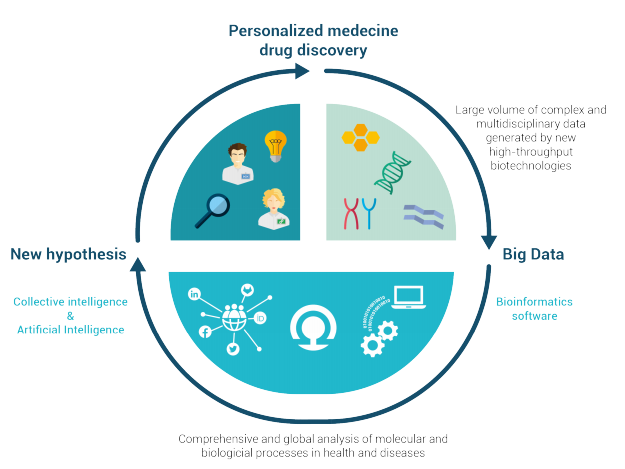
\includegraphics[width=0.7\textwidth]{poglavlja/1/slike/Primena.png}
\end{figure} 

Bioinformatika je spoj više različitih disciplina, kao što su:
\begin{itemize}
	\item Statistika
	\item Istraživanje podataka	
	\item Računarstvo
	\item Računarska biologija
	\item Biologija
	\item Biostatistika
\end{itemize}
Prikaz preklapanja ovih disciplina možemo videti na slici 1.2.
\begin{figure}[h]
\caption{Preklapanjem različitih disciplina dobijamo bioinformatiku.}
\centering
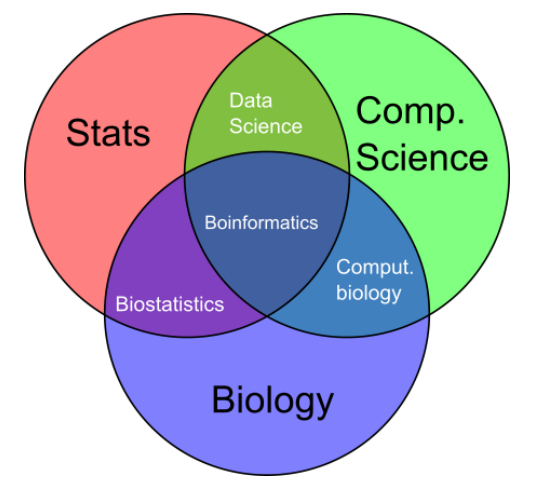
\includegraphics[width=0.7\textwidth]{poglavlja/1/slike/Multidisciplinarnost.png}
\end{figure}  

\newpage

\section{Replikacija genoma}
\label{sec:replikacija}

\subsection{DNK}

Dezoksiribonukleinska kiselina (akronimi DNK ili DNA, od engl. \textit{ deoxyribonucleic acid}), nukleinska kiselina koja sadrži uputstva za razvoj i pravilno funkcionisanje svih živih organizama. Zajedno sa RNK i proteinima, DNK je jedan od tri glavna tipa makromolekula koji su esencijalni za sve poznate forme života. \\\\
Sva živa bića svoj genetički materijal nose u obliku DNK, sa izuzetkom nekih virusa koji imaju ribonukleinsku kiselinu (RNK). DNK ima veoma važnu ulogu ne samo u prenosu genetičkih informacija sa jedne na drugu generaciju, već sadrži i uputstva za građenje neophodnih ćelijskih organela, proteina i RNK molekula. DNK segment koji sadrži ova važna uputstva se naziva gen.\\\\

DNK se sastoji iz dva polimerna lanca koji imaju antiparalelnu orijentaciju, i svaki od njih je sastavljen od azotnih baza:
\begin{itemize}
	\item adenin (A)
	\item timin (T)
	\item guanin (G)
	\item citozin (C)
\end{itemize}

\begin{figure}[h]
\caption{Prikaz DNK, slika preuzeta sa https://ghr.nlm.nih.gov/primer/basics/dna}
\centering
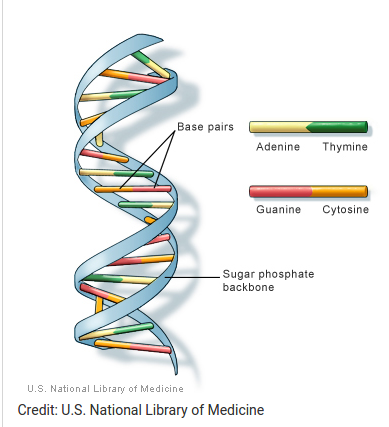
\includegraphics[width=0.5\textwidth]{poglavlja/1/slike/DNK.png}
\end{figure} 

Lanci DNK su međusobno spojeni i to tako da se veze uspostavljaju isključivo između adenina i citozina ili između guanina i timina. Na osnovu toga, ako nam je poznat sastav jednog lanca, lako možemo zakljuciti i sastav drugog lanca, zbog čega se kaže da su DNK lanci \textbf{međusobno komplementarni}.\\\\
Da bismo lakše manipulisali sa informacijama koje DNK nosi i približili sadržaj računarskoj struci, DNK ćemo posmatrati kao nisku nad azbukom \textit{A,C,G,T}.

\subsection{Replikacija genoma u ćeliji}
Replikacija genoma je jedan od najvažnijih zadataka ćelije. Pre nego što se podeli, ćelija mora da najpre replicira svoj genom, tako da svaka od ćerki ćelija dobije svoju kopiju. \\\\
Dzejms Votson (engl. \textit{James Watson}) i Fransis Krik (engl. \textit{Fransis Crick}) su 1953. godine napisali rad u kome su primetili da postoji mehanizam za kopiranje genetskog materijala. Oni su uočili da se lanci roditeljskog DNK molekula odvijaju tokom replikacije i da se, potom, svaki lanac ponaša kao uzorak za sintezu novog lanca (na osnovu toga što se uvek spajaju iste aminokiseline A-C i G-T, rekreiranje lanca je moguće). Kao rezultat ovakvog ponašanja, proces replikacije počinje parom komplementarnih lanca i završava se sa dva para komplementarnih lanaca, kao što se može videti na slici ispod.\\\\

\begin{figure}[h]
\caption{Prikaz replikacije}
\centering
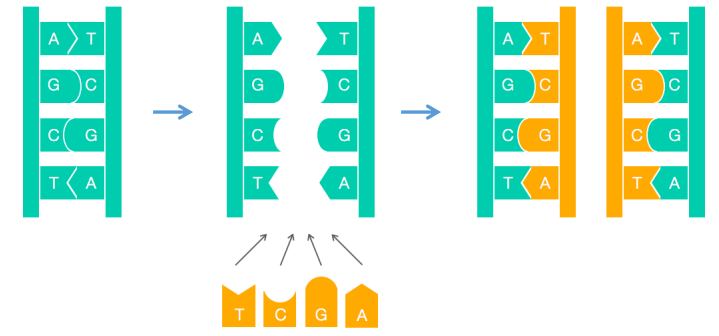
\includegraphics[width=1\textwidth]{poglavlja/1/slike/Replikacija.png}
\end{figure} 

Replikacija počinje u regionu genoma koji se naziva \textbf{početni region replikacije} (skraćeno \textit{oriC}), izvode je enzimi koje se nazivaju DNK polimeraze, koje predstavljaju mašine za kopiranje na molekularnom nivou.\\\\
Nalaženje početnog regiona replikacije predstavlja veoma važan problem, ne samo za razumevanje funkcionisanja kako se ćelije repliciraju, već je koristan i u raznim biomedicinskim problemima. Na primer, neki metodi genskih terapija uključuju genetski izmenjene mini genome, koji se zovu virusni vektori, zbog svoje sposobnosti da prodru kroz ćelijski zid (poput pravih virusa). Virusni vektori u sebi nose veštačke gene koji unapredjuju postojeći genom. Genska terapija je prvi put uspešno izvršena 1990. godine na devojčici koja je bila toliko otporna na infekcije da je bila primorana da živi isključivo u sterilnom okruženju.\\\\
Osnovna ideja genske terapije je da se pacijent, koji pati od nedostatka nekog bitnog gena, zarazi viralnim vektorom koji sadrži veštački gen koji enkodira terapeutski protein. Jednom kad je unutar ćelije, vektor se replicira, što dovodi do lečenja bolesti pacijenta. Da bi moglo da dodje do ovoga, biolozima je neophodno da znaju gde je \textit{oriC}.

\subsubsection{Kako ćelija prepoznaje \textit{oriC}?}
Pitamo se kako ćelija prepoznaje oriC? Sigurno je da postoji neka niska aminokiselina koja označava oriC, ali kako ga prepoznati?\\\\
Ograničimo se na bakterijski genom, koji se sastoji od jednog kružnog hromozoma. Istraživanje je pokazalo da je region, koji predstavlja oriC kod bakterija,
dug svega nekoliko stotina nukleotida.\\\\

\begin{figure}[h]
\caption{Prikaz početka replikacije kod bakterija}
\centering
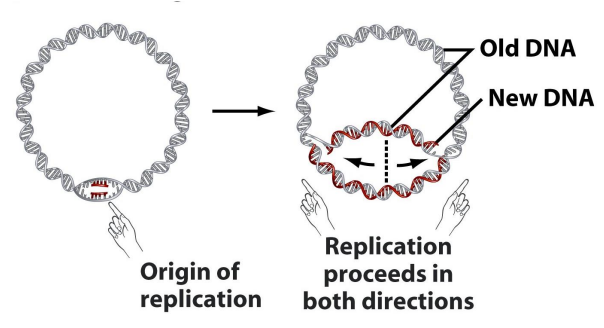
\includegraphics[width=0.7\textwidth]{poglavlja/1/slike/Replikacija_bakterija.png}
\end{figure} 

Poznato je da DNKA utiče na početak replikacije. \textit{DNKA} je protein koji se vezuje na kratki segment unutar oriC, poznatiji kao \textbf{DNKA boks}. Ona predstavlja poruku unutar sekvence DNK koja govori proteinu DNKA da se veže baš tu. Postavlja se pitanje kao pronaći taj region bez prethodnog poznavanja izgleda DNKA boks? \\\\

Da bismo bolje razumeli \textit{problem skrivene poruke} uzmimo za primer priču Edgara Alana Poa - $"$Zlatni jelenak$"$ (engl. \textit{$"$The Gold-Bug$"$}).
Naime, u toj priči jedan od likova, Vilijam Legrand (engl. \textit{William Legrand}), treba da dešifruje poruku :\\

\texttt{53++!305))6*;4826)4+.)4+);806*;48!8`6
0))85;]8*:+*8!83(88)5*!;46(;88*96*?;8\\
)*+(;485);5*!2:*+(;4956*2(5*4)8`8*;40
69285);)6!8)4++;1(+9;48081;8:8+1;48!8
5;4)\\485!528806*81(+9;48;(88;4(+?34;48
)4+;161;:188;+?;}\\\\
On uočava da se $"$;48$"$ pojavljuje veoma često, i da verovatno predstavlja $"$THE$"$, najčešću reč u engleskom jeziku. Znajući to, zamenjuje karaktere odgovarajućim slovima i postepeno dešifruje celu poruku.\\\\
\texttt{53++!305))6*THE26)H+.)H+)806*THE
!E`60))E5;]E*:+*E!E3(EE)5*!TH6(T
EE*96*?;E)*+\\(THE5)T5*!2:*+(TH956
*2(5*H)E`E*TH0692E5)T)6!E)H++T1(
+9THE0E1TE:E+1\\THE!E5T4)HE5!52880
6*E1(+9THET(EETH(+?34THE)H+T161T
:1EET+?T}\\\\
Želeli bismo da ovaj princip primenimo na naš problem nalaska \textit{oriC}-a. Ideja je da uvidimo da li postoje reči koje se neuobičajeno često pojavljuju. Uvedimo termin k-gram da označimo string dužine $k$ i COUNT(Text, Pattern) da označimo broj puta kojih se k-gram $Pattern$ pojavio u tekstu $Text$. Osnovna ideja je da pomeramo prozor, iste dužine kao k-gram $Pattern$, niz tekst, usput proveravajući da li se pojavljuje $Pattern$ u nekome od njih. 

\begin{lstlisting}
PATTERNCOUNT(Text, Pattern)
	count = 0
	for i = 0 to |Text| - |Pattern|
		if Text(i,|Pattern|) = Pattern
			count = count + 1 
	return count
\end{lstlisting}
	
Za neki $Pattern$ kažemo da je on \textit{najčešći k-gram} u tekstu $Text$, ako je njegov $COUNT$ najveći među svim k-gramima. Na primer, \textbf{ACTAT} je najčešći 5-gram u tekstu $Text$ = ACA\textbf{ACTAT}GCA\textbf{ACTAT}CGGGACA\textbf{ACTAT}CCT, a \textbf{ATA} je najčešći 3-gram u $Text$ = CG\textbf{ATATA}TCC\textbf{ATA}G.\\\\
Sada, problem pronalaska čestih reči možemo posmatrati kao računarski problem:\\
\begin{tcolorbox}
\textbf{Problem čestih reči:} Pronaći najčešće k-grame u niski karaktera.\\
\textit{Ulaz:} Niska Text i ceo broj k.\\
\textit{Izlaz:} Svi najčešći k-grami u niski Text. \\\\
\end{tcolorbox}
Osnovni algoritam za pronalazak čestih k-grama u stringu $Text$ proverava sve k-grame koji se pojavljuju u tom stringu (takvih k-grama ima $|Text|-k+1$) i potom izračunava koliko puta se svaki k-gram pojavljuje. Da bismo implementirali ovaj algoritam, moramo da izgenerišemo niz $COUNT$, gde je $COUNT(i) = COUNT(Text, Pattern)$ za $Pattern = Text(i,k)$.\\

\begin{lstlisting}
FrequentWords(Text, k)
	FrequentPatterns <- an empty set
	for i = 0 to |Text| - k
		Pattern <- the k-mer Text(i,k)
		COUNT(i) <- PatternCount(Text, Pattern)
	maxCount <- max value in array COUNT
	for i = 0 to |Text| - k
		if COUNT(i) = maxCount
			add Text(i,k) to FrequentPatterns
	remove duplicates from FrequentPatterns
	return FrequentPatterns
\end{lstlisting}

Pitamo se, sada, kolika je složenost ovakvog pristupa?\\
Ovaj algoritam, iako uspešno nalazi ono što se od njega traži, nije najefikasniji. S obzirom na to da svaki k-gram zahteva $|Text|-k+1$ provera, svaki od njih zahteva i do $k$ poređenja, pa je broj koraka izvršavanja funkcije $PatternCount(Text, Pattern)$ zapravo $(|Text|-k+1)*k$. Osim toga, $FrequentWords$ mora pozvati $PatternCount$ $|Text|-k+1$ puta (po jednom za svaki k-gram teksta), tako da je ukupan broj koraka \textit{$(|Text|-k+1)*(|Text|-k+1)*k$}.\\Iz navedenog, možemo zaključiti da je ukupna cena izvršavanja algoritma $FrequentWords$ \textbf{$O(|Text|^2*k)$}.

\subsubsection{Primer: Pronalazak čestih reči kod bakterije \textit{Vibrio cholerae}} 

Posmatrajmo, najpre, tablicu najčešćih k-grama u \textit{oriC} regionu bakterije \textit{Vibrio cholerae}. Da li nam se čini da se neki k-grami pojavljuju neuobičajeno često?\\ 

\begin{figure}[h]
\caption{Tablica najčešćih k-grama u \textit{oriC} regionu bakterije Vibrio cholerae}
\centering
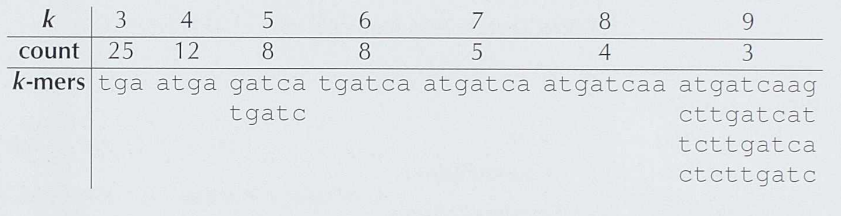
\includegraphics[width=1\textwidth]{poglavlja/1/slike/Tablica_VC.png}
\end{figure} 

Na primer, 9-gram \textbf{ATGATCAAG} se pojavljuje tri puta u \textit{oriC} regionu, da li nas to iznenađuje?\\

\begin{figure}[h]
\caption{Prikaz 9-grama ATGATCAAG i njegovog komplementa u \textit{oriC} regionu Vibrio cholerae}
\centering
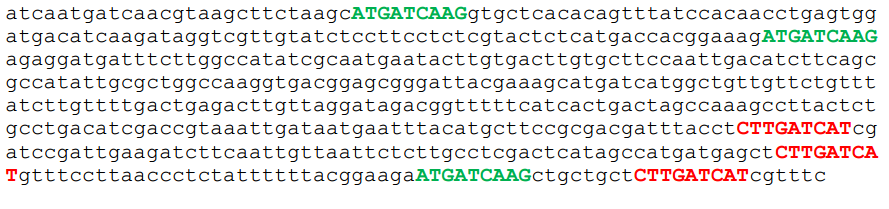
\includegraphics[width=1\textwidth]{poglavlja/1/slike/9_VC.png}
\end{figure} 

Označili smo najčešće 9-grame, umesto nekih drugih k-grama, jer je eksperimentima pokazano da su DNKA boksovi kod bakterija dugi 9 nukleotida. Verovatnoća da postoji 9-gram koji se pojavljuje 3 ili više puta u proizvoljno generisanom DNK stringu dužine 500 je $1/1300$. Uočimo da postoje četiri različita 9-grama koji se ponavljaju tri ili više puta u ovom regionu, to su: ATGATCAAG, CTTGATCAT, TCTTGATCA i CTCTTGATC.\\\\

Mala verovatnoća da se neki 9-gram toliko puta pojavi u \textit{oriC}-u kolere, govori nam da neki od četiri 9-grama koje smo pronašli može biti potencijalni DNKA boks, koji započinje replikaciju. Ali, koji?\\\\

Podsetimo se da nukleotidi A i T, kao i C i G, su komplementarni. Ako imamo jednu stranu lanca DNK i neke slobodne nukleotide, možemo lako zamisliti sintezu komplementarnog lanca, kao što se vidi na slici ispod. 

\begin{figure}[h]
\caption{Komplementarni lanci se $"$kreću$"$ u suprotnim smerovima.}
\centering
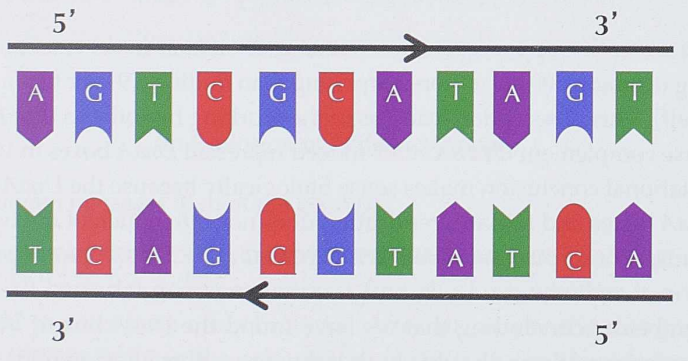
\includegraphics[width=1\textwidth]{poglavlja/1/slike/Komplementarni.png}
\end{figure} 

Posmatrajmo ponovo sliku 1.7. Na njoj možemo uočiti 6 pojavljivanja niski ATGATCAAG i CTTGATCAT, koji su zapravo komplementarni. Naći 9-gram koji se pojavljuje 6 puta u DNK nisci dužine 500 nukleotida, je još više iznenadjujuće, nego pronaći 9-gram koji se pojavljuje tri puta. Ovo posmatranje nas dovodi do toga da je ATGATCAAG (zajedno sa svojim komplementom) zaista DNKA boks Vibrio cholerae. Ovaj zaključak ima i smisla biološki, jer DNKA proteinu, koji se vezuje i započinje replikaciju, nije bitno za koji od dva lanca se vezuje.\\\\

\subsubsection{Primer: Pronalazak čestih reči kod bakterije \textit{Thermotoga petrophila}} 

Nakon što smo pronašli skrivenu poruku za Vibrio cholerae, ne bi trebalo da odmah zaključimo da je ta poruka ista kod svih bakterija. Najpre bi trebalo da proverimo da li se ona nalazi u \textit{oriC} regionu drugih bakterija, možda različite bakterije, imaju drugačije DNKA boksove. Uzmimo, za primer, \textit{oriC} region bakterije Thermotoga petrophila. Ona predstavlja bakteriju koja obitava u izrazito toplim regionima, na primer u vodi ispod rezervi nafte, gde temperature prelaze 80 stepeni Celzijusa. Pogledajmo kako izgleda \textit{oriC} region ove bakterije.

\begin{figure}[h]
\caption{Prikaz \textit{oriC} regiona Thermotoga petrophila}
\centering
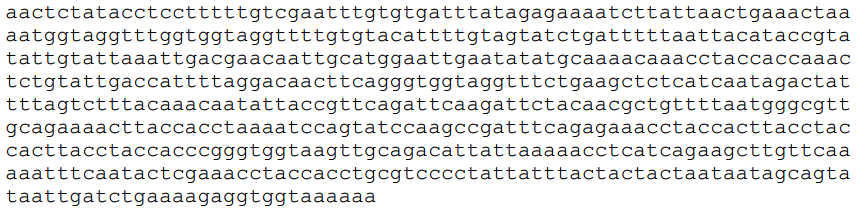
\includegraphics[width=1\textwidth]{poglavlja/1/slike/OriC_TP.png}
\end{figure} 

Možemo lako uočiti da se u ovom regionu nigde ne javljaju niske ATGATCAAG ili CTTGATCAT, iz čega zaključujemo da različite bakterije mogu koristiti različite DNKA boksove, kako bi pružile skrivenu poruku DNKA proteinu. Odnosno, za različite genome imamo različite DNKA boksove.

Najčešće reči u ovom \textit{oriC} su:
\begin{itemize}
	\item AACCTACCA, 
	\item ACCTACCAC,
	\item GGTAGGTTT,
	\item TGGTAGGTT,
	\item AAACCTACC,
	\item CCTACCACC
\end{itemize}

Pomoću alata koji se zove Ori-Finder, nalazimo CCTACCACC i njegov komplement GGTGGTAGG kao potencijalne DNKA boksove naše bakterije. Ove dve niske se pojavljuju ukupno 5 puta.

\begin{figure}[h]
\caption{Prikaz CCTACCACC i njenog komplementa u \textit{oriC} regionu Thermotoga petrophila}
\centering
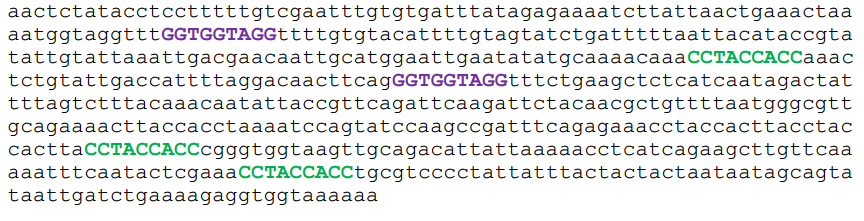
\includegraphics[width=1\textwidth]{poglavlja/1/slike/TP.png}
\end{figure} 
Naučili smo da pronađemo skrivene poruke ako je \textit{oriC}
dat, ali ne znamo da pronađemo \textit{oriC} u genomu.

\subsection{Pronalaženje početnog regiona replikacije}

Zamislimo da pokušavamo da nađemo \textit{oriC} u novom sekvenciranom genomu bakterije. Ako bismo tražili niske poput ATGATCAAG/CTTGATCAT ili CCTACCACC/GGTGGTAGG to nam verovatno ne bi bilo puno od pomoći, jer novi genom može koristiti potpuno drugačiju skrivenu poruku. Posmatrajmo, zato, drugačiji problem: umesto da tražimo grupe određenog k-grama, pokušajmo da nađemo svaki k-gram koji formira grupu u genomu. Nadajmo se da će nam lokacije ovih grupa u genomu pomoći da odredimo lokaciju \textit{oriC}-a.\\Ideja je da pomeramo prozor fiksirane dužine L kroz genom, tražeći region u kome se k-gram pojavljuje više puta uzastopno. Za L ćemo uzeti vrednost 500, koja predstavlja najčešću dužinu \textit{oriC}-a kod bakterija. \\\\
Definisali smo k-gram kao \textit{grupu}, ako se pojavljuje više puta unutar kratkog intervala u genomu. Formalno, k-gram Pattern formira (L, t) grupu unutar niske Genome ako postoji interval genoma, dužine L, u kome se k-gram pojavljuje barem t puta. \\\\
\begin{tcolorbox}
\textbf{Problem pronalaženja grupa.} Naći k-grame koji
formiraju grupe unutar niske karaktera.\\
Ulaz. Niska Genome i celi brojevi k (dužina
podniske), L (dužina prozora) i t (broj podniski u
grupi).\\
Izlaz. Svi k-grami koji formiraju (L, t)-grupe u
niski Genome.
\end{tcolorbox}

U genomu bakterije E.coli postoji 1904 različitih 9-
grama koji formiraju (500,3)-grupe. Koji od njih
ukazuje na početni region replikacije?

\subsubsection{Iskrivljeni dijagrami}

S obzirom na to da imamo veliku količinu statističkih podataka, pitamo se kako ih možemo upotrebiti da bismo došli do lokacije \textit{oriC}-a? U tome nam mogu pomoći \textbf{iskrivljeni dijagrami}(engl. \textit{skew diagram}). Osnovna ideja je da prođemo kroz genom i da računamo razliku između količine guanina(G) i citozina(C). Ako ova razlika raste, onda možemo pretpostaviti da se krećemo niz polulanac koji ide na desno (u nastavku samo polulanac, smer $5'-> 3'$), a ako razlika počne da se smanjuje, onda pretpostavljamo da smo na obrnutom polulancu ($3' -> 5'$). Zbog procesa koji se naziva deaminacija (gubljenje aminokiselina), svaki polulanac ima manjak citozina u poređenju sa guaninom, a svaki obrnuti polulanac ima manjak guanina u odnosu na citozin. 

\begin{figure}[h]
\caption{Prikaz kretanja.}
\centering
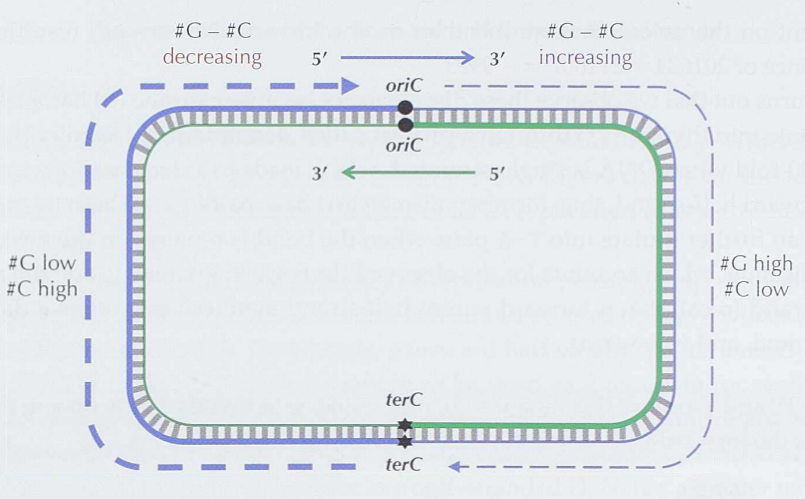
\includegraphics[width=1\textwidth]{poglavlja/1/slike/Polulanci_CG.png}
\end{figure} 

\begin{figure}[h]
\caption{Iskrivljeni dijagram genoma Genome = CATGGGCATCGGCCATACGCC.}
\centering
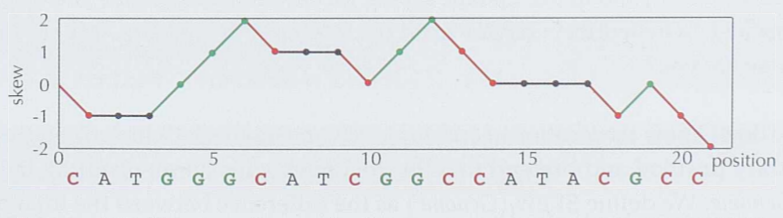
\includegraphics[width=1\textwidth]{poglavlja/1/slike/skew.png}
\end{figure} 

Posmatrajmo iskrivljeni dijagram bakterije Ešerihija Koli. Lako uočavamo minimalnu vrednost skew dijagrama.

\begin{figure}[h]
\caption{Iskrivljeni dijagram Ešerihije koli.}
\centering
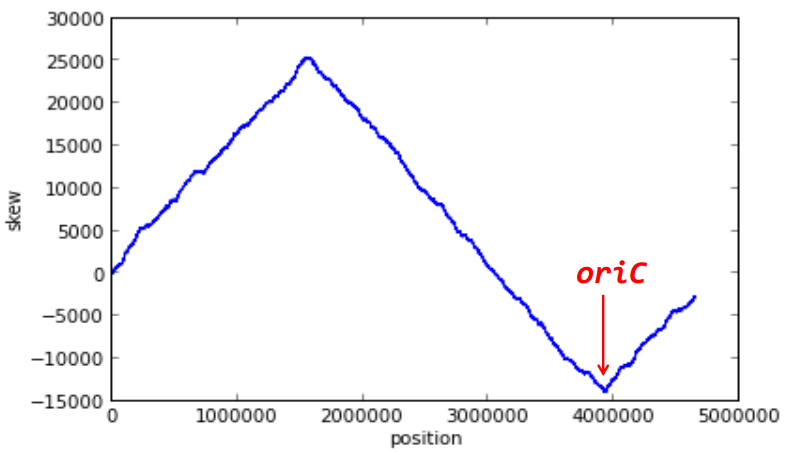
\includegraphics[width=1\textwidth]{poglavlja/1/slike/Ecoli_oriC.png}
\end{figure} 

Minimalna vrednost iz iskrivljenog dijagrama ukazuje baš na ovaj region:

\begin{figure}[H]
\caption{Region na koji pokazuje minimalna vrednost iskrivljenog dijagrama Ešerihije koli.}
\centering
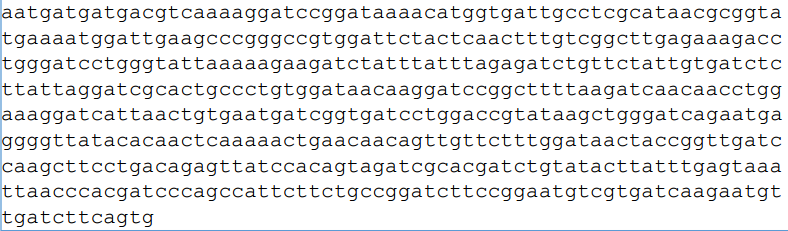
\includegraphics[width=1\textwidth]{poglavlja/1/slike/ecoli_region.png}
\end{figure} 

Uočimo da u ovom regionu nema čestih 9-grama (koji se pojavljuju 3 ili više puta). Iz toga zaključujemo da, iako smo uspeli da nađemo \textit{oriC} bakterije Ešerihija koli, nismo uspeli da nađemo DNKA boksove. Međutim, pre nego što odustanemo od potrage, osmotrimo još jednom \textit{oriC} Vibrio colerae, kako bismo pokušali da nađemo način da izmenimo naš algoritam i uspemo da lociramo DNKA boksove u Ešerihiji koli. Veoma brzo, može se uvideti da osim tri pojavljivanja ATGATCAAG i tri pojavljivanja CTTGATCAT, \textit{oriC} Vibrio cholerae sadrži i dodatna pojavljivanja ATGATCAAC i CATGATCAT koji se razlikuju samo u jednom nukleotidu od gornjih niski. Ovo još više povećava šanse da smo naišli na prave DNKA boksove, a ima i biološkog smisla. Naime, DNKA se može vezati i za nesavršene DNKA boksove, one koji se razlikuju u nekoliko nukleotida.\\\\


\begin{figure}[H]
\caption{Prikaz pojavljivanja nesavršenih niski nukleotida.}
\centering
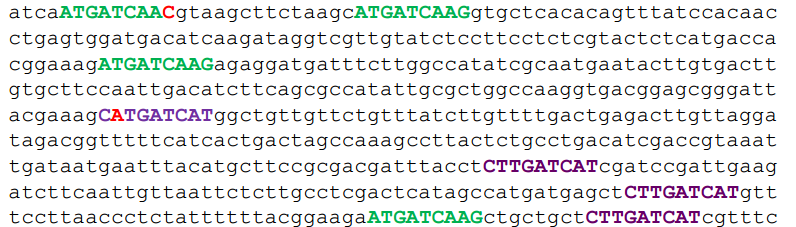
\includegraphics[width=1\textwidth]{poglavlja/1/slike/nesavrseni1.png}
\end{figure} 

Cilj nam je da sada izmenimo algoritam čestih reči (FrequentWords) tako da možemo da pronađemo DNKA boksove koji su predstavljeni čestim k-gramima, sa mogućim izmenama na pojedinim nukleotidima. Ovaj problem nazvaćemo problem čestih reči sa propustima.\\\\
\begin{tcolorbox}
\textbf{Problem čestih reči sa propustima.} Pronaći najčešće k-grame sa
propustima u niski karaktera.\\
Ulaz: Niska Text i celi brojevi k i d.\\
Izlaz: Svi najčešći k-grami sa najviše d propusta u niski Text. \\
\end{tcolorbox}
Pokušajmo, još jednom, sa pronalaskom DNKA boksova kod Ešerihije koli, tako što ćemo naći najčešće 9-grame sa propustima i komplementima u regionu \textit{oriC} koji nam je predložen minimalnom vrednošću iskrivljenog dijagrama. Pokušaćemo sa malim prozorom koji ili počinje ili se završava ili je centriran na poziciji najmanje iskrivljenosti. Ovakvim izvođenjem pronalazimo TTATCCACA/TGTGGATAA kao najčešći 9-gram. Međutim, ovo nije jedini 9-gram. Za ostale 9-grame još uvek ne znamo čemu služe, ali znamo da nose skrivene informacije, da se grupišu unutar genoma i da većina njih nema veze sa replikacijom. 

\begin{figure}[H]
\caption{Prikaz pronađenih niski sa propustima i komplementima u \textit{oriC} regionu Ešerihije koli.}
\centering
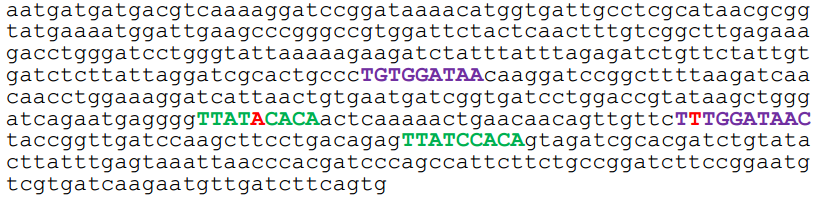
\includegraphics[width=1\textwidth]{poglavlja/1/slike/ecoli_poslednji.png}
\end{figure} 

\newpage

\section{Zadaci sa vežbi}
U nastavku će biti predstavljeni zadaci sa vežbi na kursu rađeni u programskom jeziku Python.

\subsection{FrequentWords}

\lstinputlisting[language=Python]{poglavlja/1/kodovi/1.py}

\subsection{Faster FrequentWords}

\lstinputlisting[language=Python]{poglavlja/1/kodovi/3.py}

\subsection{Skew Diagram}

\lstinputlisting[language=Python]{poglavlja/1/kodovi/4.py}

\subsection{FrequentWords With Mismatches}

\lstinputlisting[language=Python]{poglavlja/1/kodovi/5.py}


\chapter{Koji DNK šabloni igraju ulogu molekularnog sata?}
\section{Biološki problem}

Bioritam svih živih bića kotroliše "unutrašnji časovnik" koji još zovemo i cirkadijalni. Ljudi koji često putuju avionom na drugi kraj sveta mogu to da osete kada pokušaju da zaspu nakon promene nekoliko vremenskih zona. Kao i svaki sat, i ovaj može da se pokvari, što rezultuje genetskom bolešću pod nazivom sindrom odložene faze spavanja. Njegova osnova je na molekularnom nivou. Mnogi procesi su kontrolisani ovim časovnikom, što ilustruje slika 2.1. Kao što vidimo, postoji tačno određeno vreme u toku dana kada telo ima najnižu temperaturu, kada kreće i prestaje lučenje hormona poput melatonina (neophodnog za kvalitetan san) i slično.

\begin{figure}[h]
\caption{Cirkadijalni ritam}
\centering
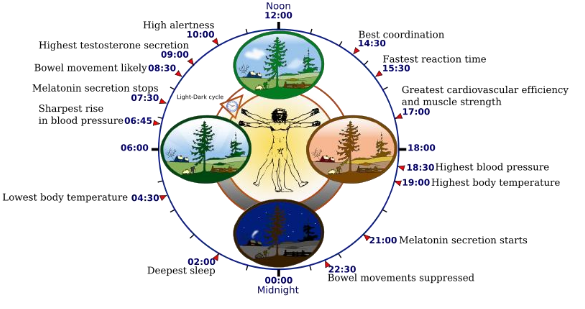
\includegraphics[width=1.1\textwidth]{poglavlja/2/slike/12cut.PNG}
\end{figure}

Naučnici su se pitali kako ćelije znaju kada treba da uspore ili ubrzaju proizvodnju određenih proteina. Ranih sedamdesetih, Ron Konopka i Sejmor Benzer su napravili prve korake ka rešavanju ove misterije. Do danas je otkriveno mnogo cirkadijalnih gena koji koordiniraju ponašanje stotine drugih gena. \\
\indent Kod čoveka, cirkadijalni ritam je promenljiv, tj. varira od osobe do osobe. Mi ćemo se u daljem tekstu fokusirati na biljke, jer je kod njih cirkadijalni ritam pitanje života i smrti, stoga ne sme biti promenljiv. Geni biljaka moraju znati kada sunce izlazi i zalazi kako bi znali kada treba vršiti fotosintezu, jer je ona od krucijalne važnosti za život biljke, a usko povezana sa količinom sunčeve svetlosti. Primeri specifičnih ponašanja nekih biljaka u zavisnosti od cirkadijalnog ritma dati su na slici 2.2.

\begin{figure}[!htb]\centering
    \caption{Cirkadijalni ritam biljke}
   \begin{minipage}{0.5\textwidth}
     \frame{
\includegraphics[width=.7\linewidth]{poglavlja/2/slike/13-1.PNG}}
   \end{minipage}
   \begin {minipage}{0.4\textwidth}
     \frame{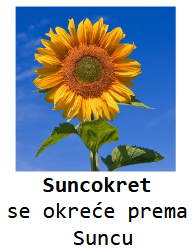
\includegraphics[width=.7\linewidth]{poglavlja/2/slike/13-2.PNG}}
   \end{minipage}
\end{figure}

Ispostavlja se da svaka ćelija biljke čuva podatak o tome da li je dan ili noć nezavisno od drugih ćelija, kao i da su samo tri gena odgovorna za upravljanje satom. Oni kodiraju regulatorne proteine (transkripcione faktore)- to su LCY, CCA1 i TOC1. Spoljašnji faktori, kao što je količina sunčeve svetlosti, kontrolišu regulatorne gene i regulatorne proteine kako bi organizmi prilagodili svoju gensku ekspresiju, odnosno da li će se protein sintetisati u to vreme ili ne. Dakle, svaki metabolički proces je regulisan cirkadijalnim časovnikom kojim upravljaju regulatorni proteini, odlučujući kada će se koji protein u ćeliji biljke sintetisati. Regulatorni proteini upravljaju genskom ekspresijom tako što se vežu za DNK u trenucima kada je potrebno sintetisati neki protein važan za cirkadijalni ritam, kao što je prikazano na slici 2.3. Naravno, to vezivanje se ne može ostvariti bilo gde u okviru DNK, već postoje posebna mesta, kao što je prikazano na slici 2.4. Ta posebnost je neophodna iz više razloga. Regulatorni protein mora znati gde treba da se veže, a isto tako DNK mora znati kako da to protumači, odnosno, to za nju mora biti signal da je vreme započeti sintezu, kao i pružiti informaciju o kom se proteinu radi. Ta posebna mesta predstavljaju manje skupove nukleotida u DNK koji nazivamo \textbf{regulatorni motivi}. Naš zadatak je da ih pronađemo. 

\begin{figure}[h]
\caption{Regulatorni proteini na delu}
\centering
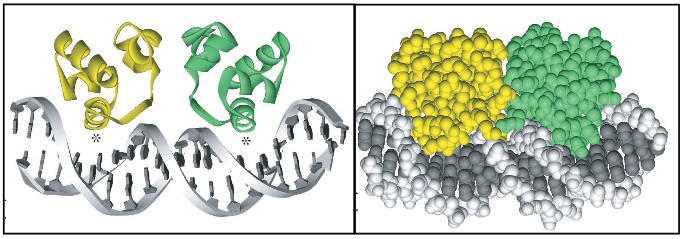
\includegraphics[width=0.55\textwidth]{poglavlja/2/slike/14.PNG}
\end{figure}

\begin{figure}[h]
\caption{Mesta vezivanja regulatornih proteina}
\centering
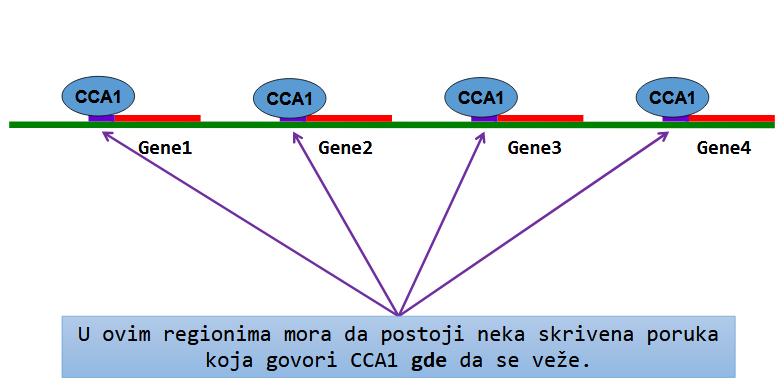
\includegraphics[width=0.7\textwidth]{poglavlja/2/slike/16.PNG}
\end{figure}

\section{Informatički problem}

Kako bismo informatički rešili problem pronalaženja regulatornih motiva u DNK, moramo predstaviti sve gorepomenute biološke pojmove na način koji bi informatičar i njegov računar mogli razumeti i obraditi. 

\begin{itemize}
    \item Iz ove tačke gledišta, DNK predstavlja nisku karaktera nad azbukom: {A, G, T, C}.
    \item Kodirajuće sekcije DNK (one koje se prepisuju i prevode u proteine) za nas će biti podniske niske DNK.
    \item Regulatorni motiv je šablon koji se pojavljuje tačno jednom u svakoj kodirajućoj sekciji DNK.
\end{itemize}

Hajde da damo u računarskom smislu korektnu definiciju problema: \\
\begin{tcolorbox}
\textbf{Informatička definicija problema nalaženja regulatornih motiva u DNK} \\
\textbf{Ulaz:} N niski koje predstavljaju kodirajuće sekvence DNK.\\
\textbf{Izlaz:} Podniska dužine k koja predstavlja regulatorni motiv (skrivenu poruku, mesto vezivanja regulatornih proteina).
\end{tcolorbox} 

Ovaj problem nas podseća na problem pronalaženja \textit{OriC}-a, koji smo rešavali svodeći ga na pronalaženje čestih reči u tekstu koristeći algoritam \textit{FrequentWords}, detaljno opisan u prethodnom poglavlju. Da bismo taj algoritam primenili ovde, neophodno je da od niza niski dobijemo konkatenacijom jednu veliku nisku, na koju ćemo primeniti ovaj algoritam. \\

Međutim, ovaj algoritam nije primenljiv ako motivi mutiraju. Možemo pokušati da primenimo algoritam \textit{FrequentWordsWithMissmatches}. To bi nas dovelo do tačnog rešenja, ali nakon previše vremena. Naime, kada smo nalazili \textit{OriC}, tražili smo uzorke dužine 9 karaktera (DnaA box je bio te dužine). U ovom slučaju, tražimo motive koji su najčešće dužine 15 karaktera, pa nam ovaj algoritam ne radi dovoljno brzo. Dakle, potrebna nam je nova ideja. 

\section{Problem ubačenog motiva}

I dalje pokušavamo da pronađemo skrivenu poruku u DNK koja kodira mesto vezivanja regulatornih proteina za DNK. Dali smo korektnu definiciju problema i, kao pravi matematičari, pokušali najpre da svedemo problem na neki drugi, koji smo već rešili. Međutim, to nas je odvelo u veliku vremensku složenost, pa samim tim i neupotrebljivost pronađenog algoritma za rešavanje. Zaključili smo da nam je potreban novi pristup, tj. da moramo probati da problem rešimo direktno - bez pomoći algoritama za \textit{OriC}. Za ovako nešto, neophodno je najpre definisati još nekoliko pojmova vezanih za šablone koje pokušavamo da pronađemo:

\begin{itemize}
    \item Mutirani šablon predstavlja šablon u kome se na nekim mestima može pojaviti mutacija, odnosno odstupanje od početne niske.
    \item $(k, d)$ motiv je k-gram koji se pojavljuje u svakoj sekvenci sa najviše $d$ razlika.
    \item Kanonski motiv predstavlja motiv koji tražimo (bez uticaja mutacija).
    \item Instance su mutirani motivi - oni koji se pojavljuju u niskama sa najviše $d$ grešaka, odnosno razlika u odnosu na kanonski motiv.
\end{itemize}

Sada, kada smo tačno i precizno definisali pojmove koji će nam igrati uloge regulatornih motiva, izmenićemo i samu definiciju problema, tj. malo promeniti scenario tako da se sve uloge lepo uklope, pazeći naravno da ne izgubimo na tačnosti definicije.

\begin{tcolorbox}
\textbf{Problem ubačenog motiva:} Pronalaženje $(k, d)$ motiva u skupu niski\\
\textbf{Ulaz:} Skup niski $Dna$ i celi brojevi $k$ (dužina motiva) i $d$ (maksimalni broj razlika).\\
\textbf{Izlaz:} Svi $(k, d)$ motivi u skupu $Dna$.
\end{tcolorbox}

Nova definicija problema izrodiće nekoliko novih ideja za njegovo rešavanje, a te ideje izrodiće nove algoritme. U daljem tekstu prikazaćemo nekoliko rešenja, uz osvrt na ideju koja nas je do njega dovela.


\subsection{Enumeracija motiva}
Početna ideja je zasnovana na gruboj sili - za svaki k-gram ćemo ispitati da li je $(k, d)$ motiv za dati skup niski. Dakle, trebalo bi generisati $4^k$ kombinacija i za svaku ispitati da li je $(k, d)$ motiv. Postavlja se pitanje da li je potrebno ispitati svih $4^k$ kandidata. 

\noindent Pogledajmo na primer sledeći skup niski:\\
\textbf{AAATTTAAATTTAAATTT\\ TTTAAATTTAAATTTAAA\\}
Da li ima smisla proveravati 8-gram GGAAGGAA?
Naravno da nema! Karakter G se ne pojavljuje ni u jednoj niski iz našeg skupa.
Zato sigurno ne može biti traženi $(k,d)$ motiv.
Dakle, prvo možemo izbaciti kandidate koji se ne pojavljuju ni u jednoj niski iz skupa $Dna$.
Takođe, možemo primetiti da je skup instanci jednog kandidata koje se pojavljuju u ostalim niskama (ceo skup $Dna$, bez niske u kojoj je dati kandidat podniska) prilično ograničen. Ograničenje nameće broj $d$. Dakle, jasno je da treba proveravati samo one instance koje se od kandidata razlikuju na najviše $d$ pozicija. 
Ovako redukovana pravila potrage iznedriće algoritam koji se naziva \textit{MotifEnumeration}, koji bismo u obliku pseudokoda predstavili na sledeći način:

\begin{lstlisting}
MotifEnumeration(Dna, k, d)
	for each k-mer a in Dna
    	generate all possible k-mers a1 differing from a by at most d mutations
    	for each such k-mer a1
    	    if a1 is a (k, d)-mer in each sequence in Dna
    	        output a1
\end{lstlisting}

\noindent Ovaj algoritam je suviše spor kada su $k$ i/ili $d$ veliki brojevi. Hajde da malo analiziramo složenost ovog algoritma. Možemo videti da najveću (i jedinu) komponentu složenosti čini dvostruka for-petlja, koja zavisi od broja kandidata koje pretražujemo i broja njihovih instanci. Kada su $k$ i/ili $d$ veliki brojevi, instanci ima mnogo, i pretraga ide sporo. Zbog toga, u praksi, ovaj algoritam ne pokazuje dobre rezultate za velike vrednosti $k$ i/ili $d$.
Dakle, potrebna nam je nova ideja.

\subsection{Najsličniji k-grami u parovima niski}

Videli smo da pretraga grubom silom ima veliku složenost, usled (iako redukovanog ali i dalje ogromnog) broja kandidata i njihovih instanci. Pokušali smo da redukujemo broj provera i nismo postigli mnogo. To nas dovodi do razmišljanja da ključ rešenja optimalnog algoritma ne leži u broju, već možda u redosledu. Hajde da konstruišemo ovakav primer: \\
\textbf{atcgtcagAAATTTAAAGGGgtcaactg \\
ggatcaagctAAATCTAAAGGGcttcag \\
gatctacccaAAACTTAAAGGGgtaaac \\}
Velikim slovima predstavljen je (12,1)-motiv koji tražimo. Grubom silom pretraga bi počela na samom početku prve niske. Kako naš motiv počinje na 9. poziciji prve niske, vidimo da bi 8 puta naleteli na ćorsokak. To znači da bi se 8 velikih iteracija izvršilo uzalud. Ako bismo nekako mogli početi od devete pozicije, uštedeli bismo vreme. Ali, kako da znamo koja je tajna pozicija od koje treba krenuti? Primećujemo da se podniske atcgtcag i ggatcaag prilično razlikuju (7/8 pozicija razlike). Dakle, to sigurno ne može biti sastavni deo neke instance. Medutim, podniske AAATTTAAAGGG i AAATCTAAAGGG su prilično slične (1/12 pozicija razlike). To je svakako dobar kandidat. Ako bismo u prve dve niske pronašli kandidate sa dosta sličnosti, šanse da smo odmah pogodili $(k,d)$ motiv bi bile velike. Sve i da nismo, ovim putem ćemo obilaziti prvo verovatnije kandidate, pa bi ukupan broj pretraga sa velikom verovatnoćom bio dosta manji. Dakle, možemo probati da poredimo parove niski iz $Dna$, da uočimo dva najsličnija k-grama u dve niske iz $Dna$, od njih napravimo kanonski, i za njega proveravamo da li je $(k, d)$ motiv. Malo veći primer možete videti na slici 2.5 i probati sami da nađete ubačeni motiv.

\begin{figure}[h]
\caption{Najsličniji k-grami u parovima niski - primer}
\centering
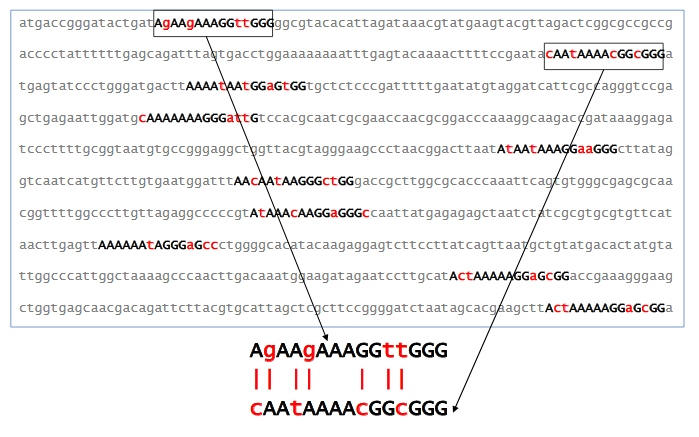
\includegraphics[width=0.9\textwidth]{poglavlja/2/slike/25.PNG}
\end{figure}

Zvuči predobro da bi bilo istinito? Pa možda ste i u pravu. 
Sličnost para niski je takođe određena brojem $d$. One se od kanonskog motiva mogu razlikovati na $d$ pozicija, što znači da se među sobom, mogu razlikovati na $2d$ pozicija.
Na malom izolovanom primeru, gde je bilo $d = 1$, zaista su slične niske isplivale kao dobri kandidati. Međutim, u praksi, sa (15,4)-motivima, broj dozvoljenih razlika je malo veći, čak 8. Kako izgledaju takvi parovi, prikazano je na slici 2.6, gde se jasno vidi koliko je to zaista mnogo i kako ove dve niske više i nisu tako slične.
\begin{figure}[h]
\caption{Najsličniji k-grami u parovima niski - problem}
\centering
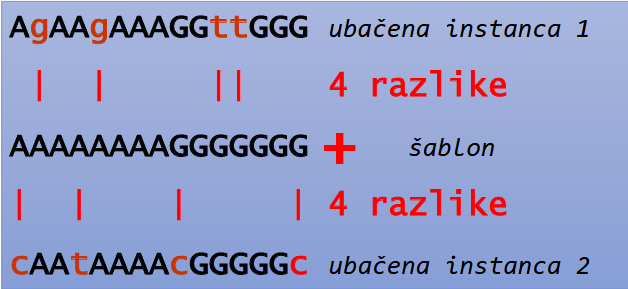
\includegraphics[width=0.9\textwidth]{poglavlja/2/slike/26.PNG}
\end{figure}

\newpage

Primer koji pokazuje koliko je ovo zaista loše rešenje je eksperiment rađen nad 10 slučajno generisanih niski iz $Dna$ dužine 600, sa ubačenim (15, 4) motivom. Pristupom pronalaženja parova niski iz $Dna$, pronađeno je nekoliko hiljada parova k-grama koji su se razlikovali na manje od 8 pozicija. Ovo sigurno nisu skrivene poruke, jer ih je previše. 

Da bismo ih pretražili u nekom smislenom redosledu, potrebno nam je da ih nekako rangiramo. Dakle, potreban nam je novi pristup.


\subsection{Matrice motiva}


Dosadašnje pretrage skupa $Dna$, nisu dale dobre rezultate. Pokušavali smo da ubrzamo pretragu na razne načine, ali bez puno uspeha. Možda je vreme da probamo da potpuno promenimo pristup, da mislimo izvan kutije. Prednost nas informatičara je u tome što ne mislimo uvek linerano. Nekada je ključ u rešenju, a ne u početnim premisama. Zbog toga, pokušajmo da analiziramo jedan skup rešenja, i da malim koracima unazad dođemo do početnih uslova.

Pretpostavićemo da imamo neku kolekciju motiva i stavimo ih u matricu. Recimo da smo uradili jednom grubu pretragu i dobili neke rezultate. Da bismo olakšali komunikaciju, uvešćemo par pojmova koje ćemo koristiti u daljem tekstu.

\begin{itemize}
    \item Najpopularniji nukleotid u nekoj koloni matrice je onaj koji se pojavljuje najveći broj puta.
    \item Konsenzus niska predstavlja nisku koja se dobija nadovezivanjem najpopularnijih nukleotida iz svake kolone.
    \item Skor predstavlja broj nepopularnih simbola (onih koji nisu najpopularniji u svojoj koloni) u matrici.
\end{itemize}

Za lakše usvajanje, ilustrovani primer ovih pojmova prikazan je na slici 2.7. Najpopularniji nukleotidi u svakoj koloni matrice motiva su napisani velikim slovima i boldovani. Oni su nadovezani u konsenzus nisku. Nepopularni simboli su napisani malim slovima, i njihov ukupan broj predstavlja skor.

\newpage

\begin{figure}[h]
\caption{Matrica motiva, konsenzus niska i skor}
\centering
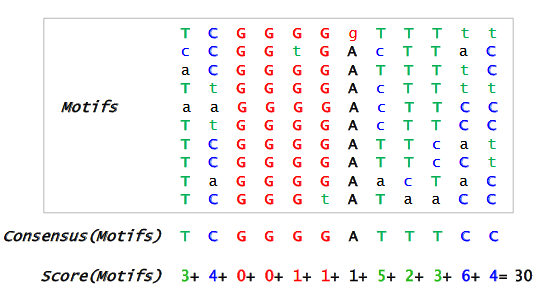
\includegraphics[width=0.9\textwidth]{poglavlja/2/slike/30.PNG}
\end{figure}

Analizirajmo malo našu matricu rešenja. Ako bismo pretpostavili da su ovo instance nekog $(k,d)$ motiva, jasno, želeli bismo da one budu što sličnije, tj. da se razlikuju na što manje pozicija. Dakle, želimo da nam broj nepopularnih simbola bude što manji, odnosno želimo mali skor. Dakle, ako ovako postavimo problem, skor je zapravo "mera neuspeha", pa je ključ dobrog rešenja u minimizovanju ove veličine. 

Novi pojmovi, novi pristup i nova ideja, zahtevaju i malo drugačiju definiciju problema:

\begin{tcolorbox}
\textbf{Problem pronalaženja motiva:} Za dati skup niski iz $Dna$ naći skup k-grama (po jedan iz svake niske) sa minimalnim skorom među svim mogućim k-gramima iz datog skupa niski.\\
\textbf{Ulaz:} skup niski $Dna$ i ceo broj $k$.\\
\textbf{Izlaz:} skup k-grama $Motifs$, po jedan iz svake niske $Dna$, tako da je vrednost skora matrice $Motifs$ minimalna.
\end{tcolorbox}

Kada smo definisali problem, vreme je da krenemo da ga rešavamo.
Prvo što nam svakako pada na pamet je gruba sila. To je obično najjednostavniji algoritam, sa ne tako dobrom brzinom. Ali, ako on da zadovoljavajuću brzinu, nema potrebe komplikovati dalje, zar ne?

Dakle, krećemo redom. Uzimamo po jedan k-gram iz svake niske skupa $Dna$ i računamo skor. Tako redom obiđemo sve kombinacije k-grama, pamteći minimalni skor, i na kraju, proglasimo rešenjem onaj skup motiva sa najmanjim skorom.

Rešenje je dobro, pa hajde da pogledamo složenost. Neka je $t$ broj niski i $n$ dužina svake niske. Zaključujemo da je $(n-k+1)$ broj k-grama jedne niske, odnosno, 
$(n-k+1)^t$ broj kombinacija koje treba da proverimo. Vreme provere je konstantno (treba samo izračunati skor i ažurirati neku vrednost). Dakle, ukupna složenost je:
$(n-k+1)^t$. Eksponencijalna složenost svakako nije dobra, tako da zaključujemo da je ovaj algoritam prespor. Moramo ga nekako unaprediti.

Vratimo se na našu matricu motiva i pokušajmo da primetimo nešto što bi nam pomoglo da malo ubrzamo stvari. Pogledajmo primer dat na slici 2.8.

\begin{figure}[h]
\caption{Matrica motiva, konsenzus niska i skor - detaljnije}
\centering
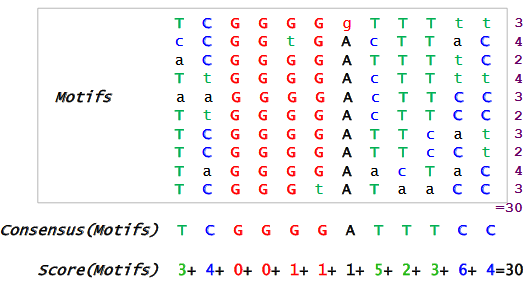
\includegraphics[width=0.9\textwidth]{poglavlja/2/slike/32.PNG}
\end{figure}

\newpage

Izračunali smo skor po vrstama i primetili da je isti kao skor po kolonama. Da li je to slučajnost? Ispostavlja se da nije. Suština veličine skor leži u tome da broji nepopularne simbole. Nije važno kako ih prebrajamo, ako su svi na broju. 
Pojam brojanja definisaćemo na malo formalniji način. Definisaćemo veličinu koja se zove Hamingonovo rastojanje.

Hamingovo rastojanje između dve niske istih dužina predstavlja broj pozicija na kojima se one razlikuju. Npr. Hamingonovo rastojanje niski AACCTTGG i ATCCATGG je 2:\\
AACCTTGG\\
ATCCATGG\\
-1--1--- = 2\\

Kada imamo Hamingovo rastojanje, možemo reći da je skor po kolonama suma Hamingovih rastojanja k-grama iz matrice od konsenzus niske. 


Vreme je da pokušamo da unapredimo naš algoritam. Želimo nekako da nađemo način da uradimo suprotno - da od konsenzus niske i niza $Dna$ dobijemo matricu $Motifs$. 
Koristićemo sledeće osobine koje smo primetili na matrici $Motifs$:
\begin{enumerate}
    \item Kako skor predstavlja sumu rastojanja od k-grama iz matrice do konsenzus niske, minimalni skor predstavlja minimizovanu sumu tih rastojanja.
    \item Kako je skor po kolononama i vrstama isti, možemo rastojanje računati i po vrstama. 
    Tako dolazimo do reforomulacije našeg problema, tj. njegovog ekvivalenta koji koristi naša nova zapažanja.
\end{enumerate}

Iskoristićemo ove osobine kako bismo još jednom predefinisali naš problem tako da odražava sliku iz novog pristupa.

\begin{tcolorbox}
\textbf{Problem pronalaženja motiva - reformulacija:} Naći k-gram $Pattern$ i skup k-grama $Motifs$ iz skupa niski $Dna$ koji minimizuju rastojanje između svih mogućim k-grama $Pattern$ i svih mogućih skupova k-grama $Motifs$.\\
\textbf{Ulaz:} skup niski iz $Dna$ i ceo broj $k$.\\
\textbf{Izlaz:} k-gram $Pattern$ i skup k-grama $Motifs$ iz skupa niski $Dna$ koji minimizuju $d(Pattern, Motifs)$.
\end{tcolorbox}

\noindent Ovo je ekvivalentno našem prethodnom problemu jer smo primetili da $d(Pattern, Motifs)$ predstavlja skor ukoliko je $Pattern$ konsenzus niska. Postavlja se pitanje da li smo ovim otežali naš problem. Ispostaviće se da nismo, jer ne moramo ispitivati sve skupove k-grama $Motifs$, već je dovoljno da iskoristimo problem niske medijane koji ispituje sve k-grame $Pattern$. 

\subsection{Problem niske medijane}
Prethodnom definicijom problema, nameće se zaključak da je sledeći prirodni korak proći kroz sve kombinacije skupa k-grama $Motifs$ i k-grama $Pattern$, kako bismo našli kombinaciju sa najmanjim rastojanjem. Međutim, videli smo i da algoritmi zasnovani na gruboj sili, tj. iscrpnoj pretrazi kombinacija u potrazi za pravom, vode ka ogromnoj složenosti i lošoj praktičnoj primeni. 

Zato ćemo ovaj put preskočiti taj korak i odmah krenuti da modifikujemo algoritam tako da dobijemo manju složenost. Primetićemo da imamo dve dimenzije pretrage (računarski bi to bile dve ugnježdene for petlje). Jedna je po svim k-gramima $Pattern$ a druga po skupovima $Motifs$. Jasno je da bi se složenost prepolovila (tj. korenovala) ako bismo imali samo jednu dimenziju. Zvuči neverovatno, ali je moguće, ako primetimo da nam unutrašnja for petlja nije potrebna, jer možemo uzeti cele niske umesto motiva. Tačnije, želimo da računamo rastojanje jednog k-grama od celog skupa $Dna$. Računanjem rastojanja od samih niski iz $Dna$ umesto od njihovim podniski dužine $k$, štedimo dosta vremena, a postižemo isti efekat. Međutim, da bismo to učinili, najpre moramo definisati nekoliko pojmova, na prvom mestu jer još uvek nismo rekli kako se računa rastojanje sem ako imamo dve niske i to iste dužine. Dakle, definisaćemo najpre sledeće pojmove: 

\begin{itemize}
    \item Hamingovo rastojanje izmedu dve niske različitih dužina predstavlja minimum Hamingovih rastojanja između kraće niske i svih podniski duže niske odgovarajuće dužine.
    \item Definišemo rastojanje između k-grama i skupa (dužih) niski kao sumu rastojanja između tog k-grama i svih niski iz skupa.
    \item Niska medijana za skup niski $Dna$ predstavlja onaj k-gram koji minimizuje rastojanje izmedu tog k-grama i skupa $Dna$ - $d(k-gram, Dna)$.
\end{itemize}

Novi pojmovi i nova ideja, prirodno vode i do nove definicije problema. Moramo dobro definisati problem koji rešavamo ako želimo da nas to dovede do dobrog algoritma za njegovo rešavanje.

\begin{tcolorbox}
\textbf{Problem niske medijane:} pronaći nisku medijanu.\\
\textbf{Ulaz:} skup niski $Dna$.\\
\textbf{Izlaz:} k-gram $k-mer$ koji minimuzuje rastojanje d($k-mer$, $Dna$).
\end{tcolorbox}

Sada imamo sav potreban alat da rešimo problem. Eliminišući jednu dimenziju, pretragu ćemo vršiti samo po svim mogućim kombinacijama k-grama $Pattern$ (njih $4^k$) i kao rezultat vratiti onaj k-gram koji ima najmanje ratojanje od skupa $Dna$. Ovaj algoritam se naziva \textit{MedianString} i prikazan je sledećim pseudokodom:

\begin{lstlisting}[escapeinside={(*}{*)}]
MedianString(Dna, k)
	best-k-mer (*$ \leftarrow $*) AAA...AA
    for each k-mer from AAA...AA to TTT...TT
        if d(k-mer, Dna) < d(best-k-mer, Dna)
            best-k-mer (*$ \leftarrow $*) k-mer
    return best-k-mer
\end{lstlisting}

Hajde da analiziramo složenost i vidimo da li smo zaista napredovali. Neka je $t$ dužina niza $Dna$ i $n$ dužina niske iz $Dna$. Tada nam je za izračunavanje rastojanja između jednog k-grama i jedne niske iz skupa $Dna$ potrebno $k \cdot (n-k+1)$ poređenja. Kako imamo $t$ niski, za izračunavanje rastojanja k-grama od skupa potrebno nam je $t \cdot k \cdot (n-k+1)$, odnosno približno $t \cdot k \cdot n$, jer je $n$ daleko veće od $k$ pa čini primarnu komponentu složenosti u $(n-k+1)$. Ceo taj postupak moramo izvršiti za svaki k-gram, odnosno $4^k$ puta, pa imamo, dakle, da ukupna složenost algoritma iznosi: $4^k \cdot n \cdot t \cdot k$. Primećujemo da je ovo dobar napredak u odnosu na $n^t \cdot k \cdot t$, ali i dalje imamo eksponencijalnu složenost. Dakle, iako je \textit{MedianString} algoritam mnogo brži od grube sile, za velike $k$ je i dalje prespor. 

\subsection{Probabilistički pristup}

\subsubsection{Uopšteno o pristupu}

Analizirali smo nekoliko determinističkih algoritama i videli da, iako uvek daju tačno rešenje, troše preveliku količinu vremena. Čak i najbolji među njima, \textit{MedianString}, imao je eksponencijalnu složenost. To nas navodi na razmišljanje da je možda ponovo došlo vreme da uradimo veliki zaokret u pristupu samom problemu i pokušamo da nađemo kompromis između tačnosti i utroška vremena. Algoritmi koji ovo omogućavaju se nazivaju probabilistički algoritmi. Oni daju tačno rešenje sa određenom verovatnoćom, ali za dosta manje vremena, i oni su naša sledeća stanica u potrazi za ubačenim motivima. Kao i svaki put kada menjamo pristup, upoznaćemo se najpre sa nekoliko osnovnih pojmova:
 
\begin{itemize}
    \item \textit{Count} matrica neke matrice motiva prikazuje koliko se puta koji nukleotid ponavlja u svakoj koloni matrice motiva.
    \item Profilna matrica neke matrice motiva prikazuje učestalost pojavljivanja nukleotida u svakoj koloni matrice motiva.
\end{itemize}

Ilustrovani primer ovih pojmova prikazan je na slici 2.9.

\begin{figure}[h]
\caption{\textit{Count} i profilna matrica}
\centering
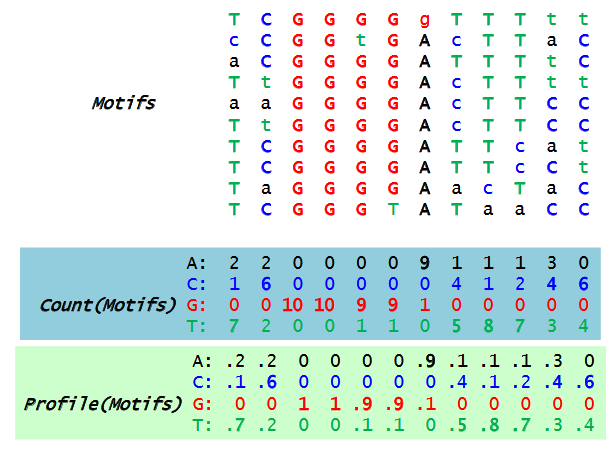
\includegraphics[width=0.9\textwidth]{poglavlja/2/slike/56.PNG}
\end{figure}

Osnovna ideja ovog pristupa može se ilustrovati bacanjem $k$ četvorostranih kockica sa otežanim stranama. Svaka kockica pretstavlja jednu poziciju u motivu dužine $k$, i na stranama ima simbole A, C, T i G. Strane kockica su otežane, tako da svaka strana pada sa onom verovatnoćom koja je zapisana u profilnoj matrici, u preseku kolone rednog broja pozicije u motivu i reda karaktera koji je na toj strani kockice. Na primer, ukoliko imamo profilnu matricu kao na slici 2.10, bacali bismo 6 četvorostranih kockica, gde bi recimo druga kockica bila otežana tako da simbol A pada sa verovatnoćom 7/8, simbol C sa verovatnoćom 0, simbol T sa verovatnoćom 1/8 i simbol G sa verovatnoćom 0. Naravno da u praksi ne možemo imati verovatnoću nula, ali sa našim zamišljenim kockicama, to je legitimna situacija. Zašto ovo nije dobro i kako se to popravlja, diskutovaćemo malo kasnije. Za sada ćemo prihvatiti ovu metaforu takvu kakva jeste i baciti naše zamišljene kockice. 
Neka su redom pali karakteri: A, T, A, C, A i G. Verovatnoću podniske koju oni čine možemo izračunati na osnovu profilne matrice, pretpostavljajući da su bacanja nezavisni događaji. Dakle, pročitaćemo iz profilne matrice verovatnoću karaktera A na prvoj poziciji (1/2), verovatnoću karaktera T na drugoj (1/8), ... , i pomnožićemo sve te vrednosti. Proizvod verovatnoća iznosi 0.001602.

\begin{figure}[h]
\caption{Računanje verovatnoće k-grama}
\centering
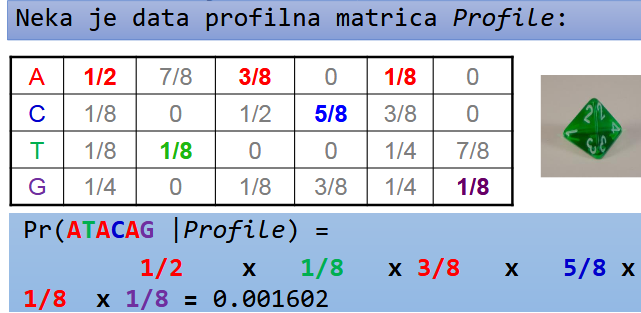
\includegraphics[width=0.5\textwidth]{poglavlja/2/slike/61.PNG}
\end{figure}

 Ako se setimo kako smo definisali matricu motiva, konsenzus nisku i profilnu matricu, lako možemo zaključiti da je ova verovatnoća zapravo verovatnoća da je niska ATACAG konsenzus niska. Sada nam same kockice više nisu potrebne, već možemo uzeti realne k-grame iz niski skupa $Dna$ i za njih računati. Na primer, za nisku CTATAAACCTTACAT iz nekog skupa $Dna$, možemo izračunati verovatnoće svih njenih podniski dužine 6 (rezultate možete videti na slici 2.11) i potražiti onaj sa najvećom verovatnoćom (u primeru sa slike 2.11 to je AAACCT). On je svakako dobar kandidat za ubačeni motiv. U ovome leži sama suština svih probabilističkih algoritama za traženje ubačenih motiva.

\begin{figure}[h]
\caption{Primer: najverovatniji 6-gram}
\centering
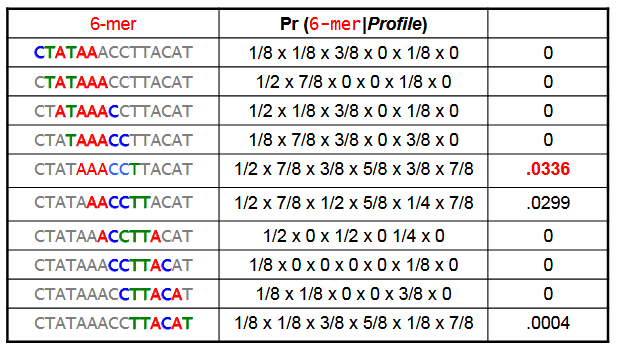
\includegraphics[width=0.8\textwidth]{poglavlja/2/slike/63-2.PNG}
\end{figure}

U daljem tekstu, predstavićemo nekoliko probabilističkih algoritama za rešavanje problema ubačenih motiva. Opisaćemo same algoritme, ali i diskutovati o njihovim dobrim i lošim stranama.

\noindent \textbf{Važna napomena}: Kao što smo već napomenuli, cenu malog vremena ovi algoritmi plaćaju tačnošću. Dakle, rešenje može malo odstupati od traženog. Zbog toga, za postizanje najbolje tačnosti, probabilističke algoritme treba pokretati više puta i uzeti najbolji rezultat.

\subsubsection{Algoritam \textit{Greedy motif search}}
Prvi algoritam koji ćemo predstaviti je pohlepni algoritam. Kao ulaz, on prima skup niski $Dna$, broj njegovih elemenata $t$ i dužinu ubačenog šablona $k$, a kao izlaz daje matricu ubačenih motiva $BestMotifs$. Suština algoritma leži u njegovom imenu: grabi k-mere iz jedne niske redom, na osnovu svakog od njih nađi najbolju matricu u koju se on uklapa, i uzmi onu koja ima najmanji skor.
Na početku $BestMotifs$ se inicijalizuje na $t$ podniski dužine $k$, od kojih svaka predstavlja prvih $k$ karakera jedne niske iz skupa $Dna$. Iterira se kroz prvu nisku skupa $Dna$, i iteracija ima onoliko koliko ima podniski dužine $k$ u njoj. U svakoj iteraciji, računa se po jedna matrica motiva. Građenje te matrice je jedan vid pohlepe ovog algoritma. Grabimo već izračunate vrednosti, kako bismo što bolje odredili sledeće. Prvi red čini tekuća podniska iteracije (podniska prve niske skupa $Dna$ koja počinje od karaktera na poziciji rednog broja iteracije). Za svaki sledeći red se pravi profilna matrica prethodno izračunatih redova i na osnovu nje računa najverovatnija podniska iz one niske skupa $Dna$, koja ima redni broj isti kao redni broj reda matrice koji računamo. Dakle, svaki sledeći motiv u matrici se sve lepše poklapa sa ostatkom matrice. Sledeći korak u iteraciji je da izračunamo skor i ako je manji, da ažuriramo vrednost $BestMotifs$. Dakle, ona matrica koja ima najmanji skor je tražena matrica $BestMotifs$. Sam algoritam ilustrovan je sledećim pseudokodom:


\begin{lstlisting}[escapeinside={(*}{*)}]
GreedyMotifSearch(Dna, k, t)
	BestMotifs (*$ \leftarrow $*) motif matrix formed by first k-mers in each string from Dna
	for each k-mer Motif in the first string from Dna
	    Motif(*$_1 \leftarrow $*) Motif
	    for i = 2 to t
	        form Profile from motifs Motif(*$_1$*), ..., Motif(*$_{i-1}$*)
	        Motif(*$_i  \leftarrow $*) Profile - most probable k-mer in the i-th string in Dna
	   Motifs (*$ \leftarrow $*) (Motif(*$_1$*), ..., Motif(*$_t$*))
	   if Score(Motifs) < Score(BestMotifs)
	        BestMotifs (*$ \leftarrow $*) Motifs
    return BestMotifs
\end{lstlisting}

\textit{GreedyMotifSearch} je brži od \textit{Median string} algoritma. Povoljan je i za veće $k$, ali cena toga je manja tačnost. Tačnost se može poboljšati primenom Laplasovog pravila, o kojem će biti nešto više reči malo kasnije.

\subsubsection{\textit{Randomized motif search}}
Posmatrajući algoritam \textit{GreedyMofifSearch}, možemo primetiti da nismo postigli pun potencijal po pitanju prelaska na probabilistički pristup. Broj iteracija je i dalje fiksan (zavisi isključivo od dužine niski iz skupa $Dna$ i dužine ubačenog motiva), a i sam njihov redosled je nametnut deterministički. Kako uvek krećemo od istog skupa motiva, i pratimo iste utabane korake, pokretanjem ovog algoritma više puta nećemo poboljšati ni tačnost ni vreme konvergencije. 
Hajde da pokušamo da potpuno izbacimo determinizam iz priče i da pustimo da izgled same niske $Dna$ i zakon verovatnoće igraju glavne uloge u konvergenciji algoritma. Prva ideja o poboljšanju probabilizma bi mogla biti vezana za sam početak algoritma. Hajde da umesto kretanja od početnih pozicija, krećemo od nekih nasumično odabranih. To sasvim sigurno donosi malo probabilizma u našu priču. Međutim, i dalje imamo iteriranje po jednoj od niski, što fiksira i broj iteracija i njihov redosled. To je ono što nam najviše i smeta. 
Na početku sekcije o probabilističkim algoritmima, naučili smo da pravimo profilnu matricu od matrice motiva, a u algoritmu \textit{GreedyMofifSearch} smo videli da je moguće i obrnuto. To je dobra ideja za osnovu iteracije. Od matrice motiva bismo mogli praviti profilnu matricu, a od profilne matrice ponovo matricu motiva. Ponavljanjem tog postupka, mogli bismo iterirati bez potrebe da se vezujemo za bilo kakav redosled podniski u nekoj od niski iz $Dna$. Ostalo je još da razmislimo kako bismo znali kada da stanemo. Pretpostavljajući da krećemo od neke nasumične matrice motiva sa lošim, tj. velikim skorom, pretpostavljajući da se krećemo ka dobrom rešenju koje ima mali skor, kao i da to činimo postepeno gradeći sve bolja, tj. verovatnija rešenja pomoću profilnih matrica, prirodno je da pomislimo da će se skor smanjivati iz iteracije u iteraciju. Dakle, iteriraćemo dokle god nam se skor smanjuje.
Ova ideja je zapravo osnova algoritma \textit{RandomizedMotifSearch}. Njegova suština leži u tome da u velikom broju iteracija ažuriramo matricu motiva i profilnu matricu tako da dobijamo sve verovatniji skup motiva, zaustavljajući se kada postignemo najniži skor. Ovaj algoritam je ilustrovan sledećim pseudokodom:

\begin{lstlisting}[escapeinside={(*}{*)}]
RandomizedMotifSearch(Dna, k, t)
    randomly select k-mers Motifs = (Motif(*$_1$*), ..., Motif(*$_t$*)) in each string from Dna
    bestMotifs (*$\leftarrow$*) Motifs
    while forever
        Profile (*$\leftarrow$*) Profile(Motifs)
        Motifs (*$\leftarrow$*) Motifs(Profile, Dna)
        if Score(Motifs) < Score(bestMotifs)
            bestMotifs (*$\leftarrow$*) Motifs
        else 
            return bestMotifs
\end{lstlisting}

Radi lakšeg razumevanja, hajde da ilustrujemo rad ovog algoritma na jednom primeru. Jedan takav, dosta uprošćen primer možemo videti na slici 2.12. Prikazan je algoritam \textit{RandomizedMotifSearch} koji konvergira u jednoj iteraciji.
Neka je dat skup $Dna$ od 5 niski dužine 10 karaktera, sa ubačenim (4,1) motivom. Na slici 2.12. u gornjem levom uglu, prikazan je skup $Dna$, tako što su velikim slovima ispisani karakteri instanci ubacenog motiva: ACCT, ATGT, GCGT, ACGA i AGGT, crnom bojom označene mutacije na motivima, a plavom nemutirani karakteri motiva. Prvi korak jeste određivanje početne vrednosti matrice \textit{Motifs}. Odabraćemo slučajno 5 pozicija (u opsegu od 1 do 7) na kojima će početi 4-grami kojima ćemo inicijalizovati matricu \textit{Motifs}, i neka su to pozicije 7, 5, 1, 2 i 7. 4-grami koji počinju na ovim pozicijama: taac, GTct, ccgG, acta i AGGT, čine početnu matricu \textit{Motifs}, koja je prikazana na slici 2.12. u gornjem centralnom delu. Sledeći korak jeste izgradnja profilne matrice na osnovu matrice \textit{Motifs}. Prebrajanjem svakog karaktera u svakoj koloni matrice \textit{Motifs} možemo odrediti \textit{count} matricu, a zatim deljenjem svakog broja iz \textit{count} matrice sa brojem niski, tj. 5 u našem primeru, dobijamo profilnu matricu. Kako izgleda profilna matrica u našem primeru, može se videti na slici 2.12 u gornjem desnom uglu. Sada kada imamo profilnu matricu, možemo izračunati nove najverovatnije motive u niskama iz $Dna$, i ažurirati matricu \textit{Motifs}. Postupak računanja matrice motiva prikazan je na slici 2.12 u središnjem delu. Za svaku nisku iz skupa $Dna$, odredićemo verovatnoće svih njenih podniski, na osnovu profilne matrice, i iz svake niske odabrati po jednu koja ima najveću verovatnoću (na slici su prikazane ljubičastom bojom). Sledeći korak bi bio da ponovo napravimo profilnu matricu itd. Međutim, u našem primeru, vidimo da je to kraj. Dobili smo traženo rešenje. Treba napomenuti da je ovo veštački kreiran primer i da je u praksi broj iteracija dosta veći.

\begin{figure}[h]
\caption{Primer rada algoritma \textit{RandomizedMotifSearch}}
\centering
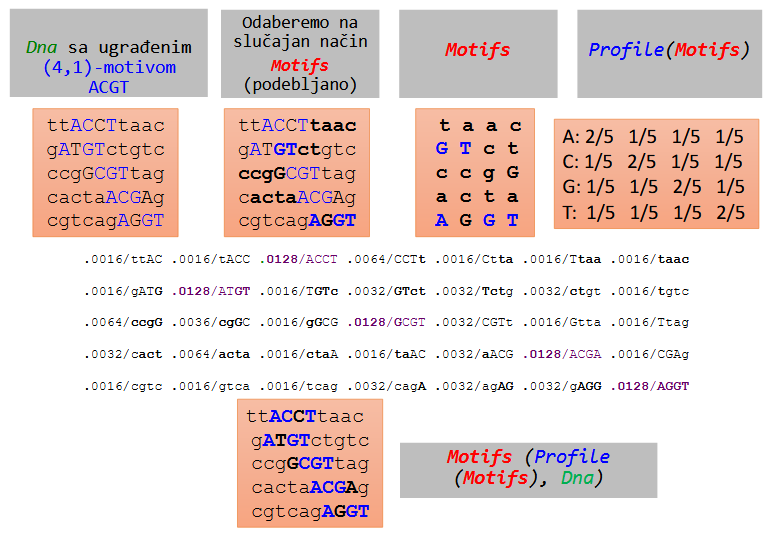
\includegraphics[width=0.8\textwidth]{poglavlja/2/slike/69.PNG}
\end{figure}

\newpage

Velika prednost ovog algoritma je u nasumičnom izboru početnog skupa motiva, što nam omogućava da ga pokrećemo iznova i izaberemo najbolje rešenje.

\subsubsection{Gibsovo sempliranje}
Algoritam \textit{RandomizedMotifSearch} je dobar i efikasan, ali ima jednu malu manu. Matrica motiva se potpuno menja iz iteracije u iteraciju, što može dovesti do toga da se izmene i neki dobro izračunati redovi. To svakako ne želimo. Ako bismo u svakoj iteraciji menjali samo po jedan motiv iz matrice, tj. posle manjih izmena pravili novu profilnu matricu i proveravali skor, mogli bismo bolje da kontrolišemo to kvarenje već nameštenih motiva. Ova modifikacija algoritma \textit{RandomizedMotifSearch} se naziva Gibsovo sempliranje. Na prvi pogled deluje kao da povećava broj iteracija i usporava konvergenciju, ali to što su promene manje, nikako ne znači da su manje i efikasne. Ako idemo pravo sitnijim koracima, stižemo brže i lakše na cilj, nego ako krupnim koracima idemo levo-desno. 
Osnovna razlika Gibsovog sempliranja u odnosu na algoritam \textit{RandomizedMotifSearch} se nalazi u sadržaju iterativnog koraka. Umesto da od cele matrice motiva pravimo profilnu matricu i na osnovu nje ažuriramo celu matricu motiva, sada ćemo nasumično odabrati jedan motiv koji ćemo izbaciti, profilnu matricu praviti od ostatka matrice, a ažuriranje matrice motiva vršiti samo nad izbačenim redom u matrici. Postupak kreiranja same profilne matrice i ažuriranja motiva je potpuno isti kao u algoritmu \textit{RandomizedMotifSearch}. Umesto pseudokodom, ovaj put ćemo algoritam prikazati u koracima:

\begin{enumerate}
    \item Formirati \textit{Motifs} izborom jednog k-grama iz svake sekvence \textbf{na slučajan način}
    \item \textbf{Na slučajan način} odabrati jedan od k-grama i ukloniti ga iz \textit{Motifs} ; označimo sekvencu kojoj taj k-gram pripada sa \textit{RemovedSequence}
    \item Kreirati profilnu matricu \textit{Profile} od preostalih k-grama u \textit{Motifs}
    \item Za svaki k-gram iz \textit{RemovedSequence}, izračunati $Pr(k-mer|Profile)$ ; na taj način dobijamo $n-k+1$ verovatnoća: $p_1, p_2, ..., p_{n-k+1}$
    \item \textbf{Bacimo kockicu} sa $n-k+1$ strana kod koje je verovatnoća da će pasti na i-tu stranu proporcionalna verovatnoći $p_i$
    \item Odredimo k-gram iz sekvence \textit{RemovedSequence} kao onaj koji ima najveću verovatnoću i dodamo ga u \textit{Motifs}
    \item Ponavljamo korake 2-6
\end{enumerate}

Radi lakšeg razumevanja, prikazaćemo i ovaj algoritam na istom primeru kao i \textit{RandomizedMotifSearch}. Skica rada algoritma je prikazana na slici 2.13.

Neka je ponovo dat isti skup $Dna$ od 5 niski dužine 10 karaktera, sa ubačenim (4,1) motivom. Na slici 2.13. u gornjem levom uglu, prikazan je skup $Dna$, tako što su velikim slovima ispisani karakteri instanci ubačenog motiva: ACCT, ATGT, GCGT, ACGA i AGGT, crnom bojom označene mutacije na motivima, a plavom nemutirani karakteri motiva. Prvi korak je isti kao i u algoritmu \textit{RandomizedMotifSearch}: određivanje početne vrednosti matrice \textit{Motifs}. Odabraćemo slučajno 5 pozicija (u opsegu od 1 do 7) na kojima će početi 4-grami kojima ćemo inicijalizovati matricu \textit{Motifs}, i neka su to pozicije 7, 5, 1, 2 i 7. 4-grami koji počinju na ovim pozicijama: taac, GTct, ccgG, acta i AGGT, čine početnu matricu \textit{Motifs}. Sledeći korak jeste izbacivanje jednog motiva. Nasumičnim izborom jednog broja iz opsega (1,5), odredili smo motiv iz reda 3 da bude izbačen. Matrica \textit{Motifs} sada izgleda kao na slici 2.13 u gornjem desnom uglu. Naredni korak je izgradnja profilne matrice na osnovu matrice \textit{Motifs}. Ovaj postupak je takođe isti kao u algoritmu \textit{RandomizedMotifSearch}, samo je skup nad kojim radimo za jedan 4-gram manji. Prebrajanjem svakog karaktera u svakoj koloni matrice \textit{Motifs} možemo odrediti \textit{count} matricu (slika 2.13, centar-desno), a zatim deljenjem svakog broja iz \textit{count} matrice sa brojem motiva, tj. 4 u našem primeru, dobijamo profilnu matricu. Kako izgleda profilna matrica u našem primeru, može se videti na slici 2.13 u donjem desnom uglu. Sada kada imamo profilnu matricu, možemo izračunati novi najverovatniji motiv u trećoj niski iz $Dna$, i ponovo popuniti treći red u matrici \textit{Motifs}. Vidimo da je podniska GCGT jedina sa pozitivnom verovatnoćom, pa samim tim i najvećom, tako da njome popunjavamo treći red matrice \textit{Motifs}. Sledeći korak bi bio da ponovo izbacimo nasumično odabrani motiv, napravimo profilnu matricu itd. Iterirali bismo sve dok skor ne prestane da se smanjuje. 


\begin{figure}[h]
\caption{Primer rada algoritma Gibsovo sempliranje}
\centering
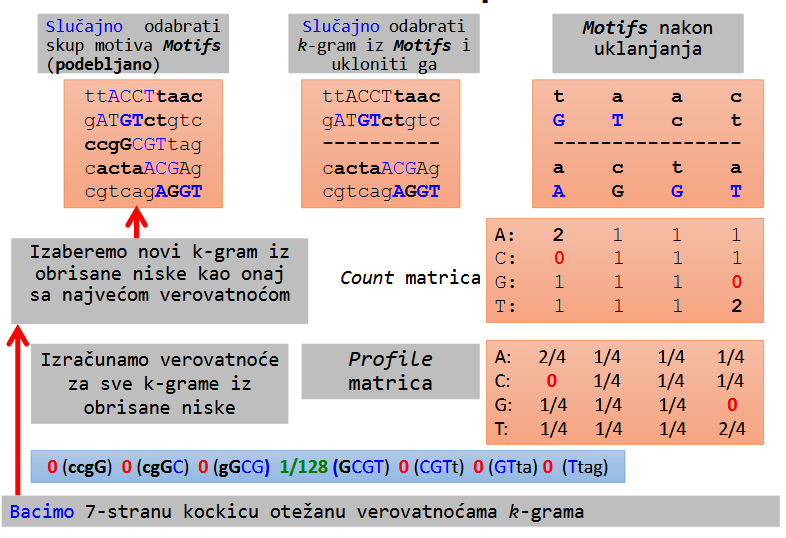
\includegraphics[width=0.8\textwidth]{poglavlja/2/slike/73.PNG}
\end{figure}

Međutim, sada ćemo se ovde zaustaviti kako bismo primetili nešto mnogo važno. Kada smo računali verovatnoće podniski kandidata za zamenu trećeg motiva, dobili smo samo jednu ne-nula vrednost od 7. To nije dobro. Jedna nula u profilnoj matrici može anulirati verovatnoće koje su sve do množenja sa njom bile prilično velike. Zbog toga one nisu baš poželjne. Ako zastanemo malo i razmislimo, shvatićemo da nisu previše ni realne, tj. da ne odražavaju realnu verovatnoću, već da su u velikom broju slučajeva uzrokovane malim obimom skupa nad kojim računamo. Zbog toga, modifikicija nula u profilnoj matrici predstavlja vrlo dobru i poželjnu modifikaciju ovog algoritma, a ta modifikacija se sprovodi korišćenjem Laplasovog pravila.

Mala napomena: Setimo se da smo već pominjali Laplasovo pravilo kao dobro poboljšanje i \textit{GreedyMofifSearch} i \textit{RandomizedMotifSearch} algoritama. Zapravo, ovo je korisna modifikacija svakog algoritma koji se zasniva na računanju profilne matrice i korišćenju njenih vrednosti.

Pre nego pređemo na modifikaciju, naglasićemo još da se prednost Gibsovog algoritma ogleda u najmanjem skoru, kao i to da je mana ovog algoritma zaglavljivanje u lokalnom minimumu usled pretrage ograničenog skupa rešenja. 

\subsubsection{Laplasovo pravilo kao poboljšanje Gibsovog semplera}

Davne 1650. godine, Oliver Kromvel je napisao:
"Molim Vas, tako Vam Hrista, mislite da je moguće da grešite". 
Ovu izjavu, je uobličio Denis Lindli i nazvao Kromvelovo pravilo:
"Traba da ostavimo malu mogućnost da Sunce sutra neće izaći".
Nešto novija replika bi se mogla naći u seriji Smolvil i rečima Leksa Lutora: "Uvek ostavljam malu mogućnost da nisam u pravu. Tako me ništa ne može iznenaditi."
Suština Kromvelog pravila leži u tome da, ukoliko potpuno odbacimo mogućnost nekog događaja, sasvim sigurno ostavljamo mogućnost pogreške. Zbog toga, treba izbegavati verovatnoće 0 i 1.

Za poboljšanje Gibsovog semplera (zapravo se može primeniti na bilo koji algoritam koji računa profilnu matricu), izvršićemo malu modifikaciju algoritma primenom Laplasovog pravila. Primenjujemo Laplasovo a ne Kromvolevo pravilo, samo iz razloga notacije i matematičkog zapisa. Laplasovo pravilo je samo preciznija (matematička) formulacija Kromvelovog pravila, sa istom suštinom. 

\begin{tcolorbox}
\textbf{Laplasovo pravilo:} U malim skupovima podataka uvek postoji šansa da se događaj koji je moguć ne desi. Slučajni algoritmi uvode pseudovrednosti koje povećavaju verovatnoće retkih događaja i eliminišu frekvencije jednake nuli zabeležene na osnovu iskustva.
\end{tcolorbox}

\indent Suština Laplasovog pravila leži u tome da, ukoliko znamo da se događaj nekada u prošlosti desio, on ne može imati verovatnoću nula. Stoga u računanje, pored vrednosti dobijenih u našem eksperimentu, ubacujemo i dve pseudovrednosti: događaj se desio i događaj se nije desio. \\

\noindent Računanje uslovne verovatnoće bez primene Laplasovog pravila bi bilo:
\begin{tcolorbox}
Ako su $X_1, ..., X_{n+1}$ uslovno nezavisne slucajne logičke promenljive (neuspeh 0, uspeh 1), tada: $Pr(X_{n+1}=1|X_1+...+X_n=s)=s/n$
\end{tcolorbox}

\noindent Računanje uslovne verovatnoće sa primenom Laplasovog pravila bi bilo:
\begin{tcolorbox}
Ako su $X_1, ..., X_{n+1}$ uslovno nezavisne slučajne logičke promenljive (neuspeh 0, uspeh 1), tada: $Pr(X_{n+1}=1|X_1+...+X_n=s)=(s+1)/(n+2)$
\end{tcolorbox}

Modifikacija Gibsovog algoritma primenom Laplasovog pravila je sadržana u dva mala koraka. Prva izmena je u okviru računanja \textit{count} matrice, gde se vrednost svakog polja uvećava za 1. To je zapravo pseudovrednost: događaj se desio. Pod događaj, podrazumeva se pojava određenog karaktera na određenoj poziciji u matrici motiva. Druga izmena je u okviru računanja profilne matrice, zato što \textit{count} matrica izgleda nešto drukčije. 

Modifikaciju Gibsovog algoritma ćemo prikazati samo na primeru, jer je skup koraka u suštini isti i ne prikazuje najbolje samu modifikaciju. Koristićemo isti primer na kome smo već demonstrirali rad Gibsovog semplera. Na slici 2.14. prkazan je rad modifikovanog Gibsovog semplera. Možemo primetiti da \textit{count} i profilna matrica izgledaju nešto drukčije (dodate su pseudovrednosti), kao i da je rezultat 7 ne-nula verovatnoća.

\begin{figure}[h]
\caption{Primer rada Gibsovog sempliranja sa primenom Laplasovog pravila}
\centering
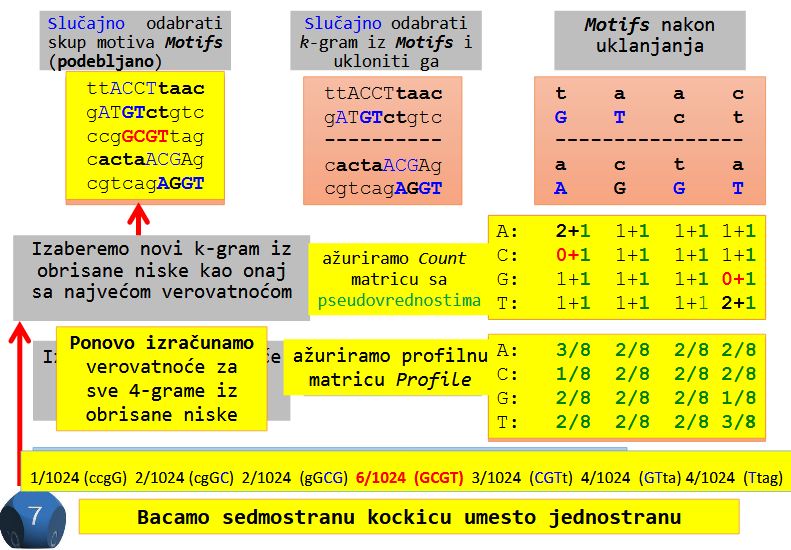
\includegraphics[width=0.7\textwidth]{poglavlja/2/slike/84.PNG}
\end{figure}

\subsection{Koji princip odabrati?}
Odgovor na ovo pitanje je - nema pravila. Nekada će se bolje pokazati jedan, a nekada drugi. Najbolje je da isprobamo više algoritama i vidimo koji se najbolje ponaša u našem slučaju. Možemo koristiti već zapažene prednosti i mane u izboru, kao na primer biranje \textit{Median string} algoritma pri malim vrednostima $k$, ali isprobavanje je ipak najpouzdaniji pristup.

\section{Zadaci sa vežbi}
U nastavku će biti predstavljeni zadaci sa vežbi na kursu rađeni u programskom jeziku \textit{Python}.

\subsection{\textit{MedianString}}

\lstinputlisting[language=Python]{poglavlja/2/kodovi/MedianString.py}

\subsection{\textit{GreedyMotifSearch}}

\lstinputlisting[language=Python]{poglavlja/2/kodovi/GreedyMotifSearch.py}

\subsection{\textit{RandomizedMotifSearch}}

\lstinputlisting[language=Python]{poglavlja/2/kodovi/RandomizedMotifSearch.py}

\subsection{\textit{GibbsSampler}}

\lstinputlisting[language=Python]{poglavlja/2/kodovi/GibbsSampler.py}


\chapter{Kako složiti genomsku slagalicu od milion delova?}

\section{Šta je sekvenciranje genoma?}

Sa biološke strane, genom jednog organizma predstavlja njegov genetski materijal. Kod većine organizama, genetski materijal je sadržan u DNK. Kod čoveka, genom sadrži oko tri milijarde nukleotida. Genomi nekih organizama su i 100 puta veći od humanog genoma. 

Sa računarske strane, genom je niska karaktera nad azbukom $\{A, C, G, T\}$.

% nije mi jasan veliki razmak koji se napravi  u tekstu na ovom mestu xD

\subsection{Kratka istorija sekvenciranja genoma}

1977. godine Walter Gilbert i Frederick Sanger razvijaju nezavisne metode sa sekvenciranje DNK, za koje su, 1098. godine, podelili su Nobelovu nagradu.
Njihove metode za sekvenciranje su bile veoma skupe - 3 milijarde dolara za sekvenciranje humanog genoma.
\\
\\
Krajem 2000-tih Sanger metodom je sekvencioniran veliki broj genoma. Visoka cena je bila ograničavajući faktor i za dalji napredak je bila neophodna nova tehnologija sekvencioniranja.
\\
\\
\textbf{NGS} predstavlja metode nove generacije sekvencioniranja. Krajem 2000-tih, na tržištu se pojavljuju nove mašine za sekvenciranje. \textit{Illumina} smanjuje trošak sekvencioniranja humanog gemona sa 3 milijarde na 10 hiljada dolara. Kompanija \textit{Complete Genomics} otvara genomsku fabriku u Silikonskoj dolini koja sekvencionira stotine genoma mesečno.
Pekinški genomski institut (BGI - Beijing Genome Institute) preuzima Complete Genomics 2013. godine i postaje najveći svetski centar za sekvenciranje genoma.
Na slici \ref{slika:cena} prikazano je kako se cena sekvencioniranja menjala godinama.


\begin{figure}[H]
	\centering
	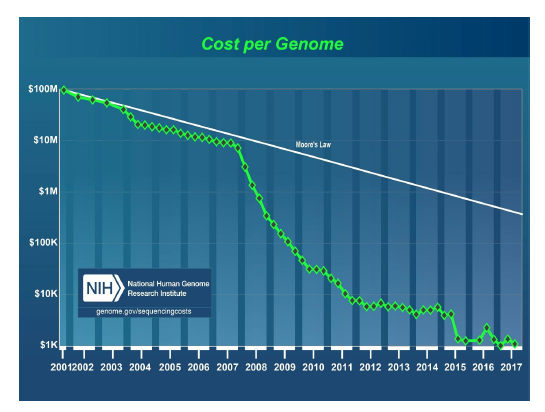
\includegraphics[width=1\textwidth]{poglavlja/3/slike/cena_sekvencioniranja.png}
	\caption{Cena sekvencioniranja kroz istoriju.}
	\label{slika:cena}
\end{figure} 



\subsection{Sekvenciranje ličnih genoma}

Genomi se kod različitih ljudi razlikuju na malom broju pozicija (u proseku sadrže jednu mutaciju na hiljadu nukleotida). Ova razlika je odgovorna za različite visine kod ljudi, da li će imati sklonost ka visokom holesterolu ili ne, za veliki broj genetskih bolesti, itd.
\\
\\
2010: Nicholas Volker je postao prvo ljudsko biće čiji je život spašen zahvaljujući genomskom sekvencioniranju.
Lekari nisu mogli da postave tačnu dijagnozu i morali su da ga podvrgnu velikom broju operacija pokušavajući da je utvrde. Sekvenciranje je otkrilo retku mutaciju na jednom genu (XIAP) koja je bila povezana sa oštećenjem njegovog imunog sistema. Ovo otkriće je navelo lekare na adekvatnu terapiju koja je rešila problem.

\section{Eksplozija u štampariji}

Zamislite da imamo hiljadu kopija istog izdanja novina na jednoj gomili, a ispod njih postavljen je dinamit. Upalimo fitilj i zamislimo da nije sve samo izgorelo već da se raspršilo u milione delića papira. Kako možemo da iskoristimo te deliće da bismo saznali koje su bile vesti iz tog izdanja? Ovaj problem nazvaćemo \textbf{Problem novina} (\ref{slika:eksplozija}). 

\begin{figure}[H]
	\centering
	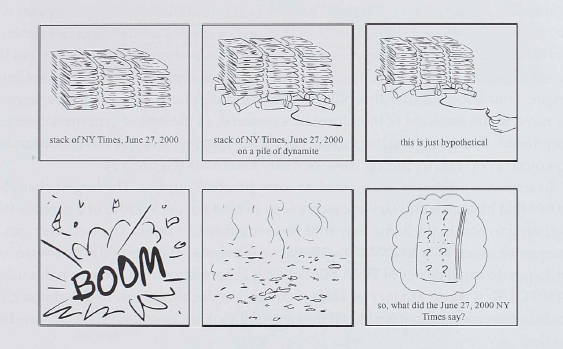
\includegraphics[width=1\textwidth]{poglavlja/3/slike/eksplozija.png}
	\caption{Problem novina poslužiće nam u razumevalju problema slaganja genoma.}
	\label{slika:eksplozija}
\end{figure} 


Problem novina je mnogo teži nego što izgleda. Kako smo imali više kopija istog izdanja, i kako smo izgubili neki deo informacija prilikom eksplozije, ne možemo samo da prilepimo deliće novina kao da su slagalica. Umesto toga, potrebno je da preklopimo delove različitih novina kako bismo rekonstruisali jedan primerak.


\begin{figure}[H]
	\centering
	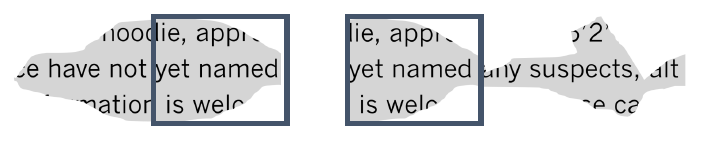
\includegraphics[width=1\textwidth]{poglavlja/3/slike/delici.png}
	\caption{Spajanje delova različitih novina koji se jednim delom preklapaju.}
	\label{slika:delici}
\end{figure} 


Kakve sad to veze ima sa našim problemom? Određivanje redosleda nukleotida u genomu, odnosno sekvenciranje genoma, predstavlja bitan problem u bioinformatici. Dužine genoma variraju: humani genom je dugačak oko 3 milijarde nukleotida, dok je genom jendoćelijskog organizma Amoeba dubia čak 200 puta duži. 


Moderne mašine za sekvenciranje (sekvenceri) ne mogu da pročitaju ceo genom nukleotid po nukleotid od početka do kraja (kao što bismo pročitali knjigu).
Mogu samo da iseckaju genom i generišu njegova kratka očitavanja. Kako to zapravo funkcioniše (\ref{slika:sekvenciranje})? Sekvencer dobija milione kopija istog genoma. Zatim vrši očitavanja čime dobijamo deliće odnosno kratke podniske. Neki delovi odnosno očitavanja biće izgubljena (kao delići novina u eksploziji, dakle gubimo deo informacija). Očitavanja su izmešana i ono što nam sekvencer daje je zapravo kolekcija podniski koje treba spojiti u jednu. Sastavljanje genoma nije isto kao i slaganje slagalice: moramo da koristimo preklapajuća očitavanja da bismo rekonstruisali genom.


\begin{figure}[H]
	\centering
	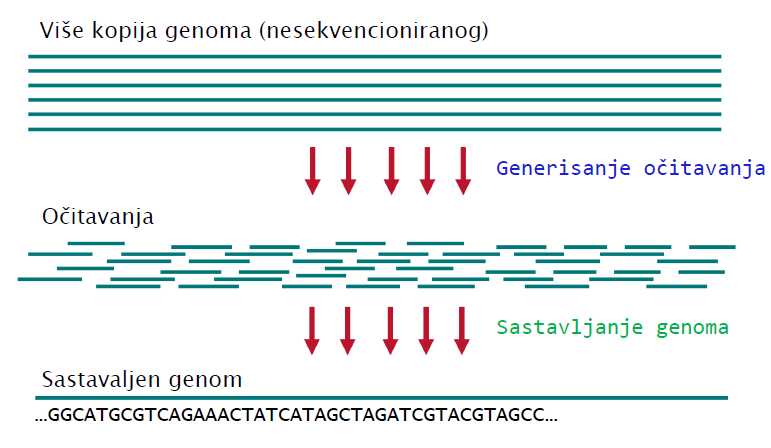
\includegraphics[width=1\textwidth]{poglavlja/3/slike/sekvencioniranje.png}
	\caption{Ilustracija problema.}
	\label{slika:sekvenciranje}
\end{figure} 


\section{Problem sekvenciranja genoma}

\begin{problem}
	[Problem sekvencioniranja genoma] Rekonstruisati genom na osnovu očitavanja.
	\\ Ulaz. Kolekcija niski Reads.
	\\ Izlaz. Niska Genome rekonstruisana na osnovu Reads.
\end{problem}

% ovo dopuniti sa snimka pošto nema ni u knjizi baš
Ovo nije dobro definisan problem. 


\subsection{k-gramski sastav niske}

k-gramski sastav niske $Text$ ($Composition_k(Text)$) predstavlja kolekcija podnsiki dužine $k$ niske $Text$, uključujući duplikate. Na primer:


% ovo sigurno može lepše xD (slajd 32)
\begin{align*}
	Composition_3(TAATGCCATGGGATGTT) =& \\
	TAA AAT ATG TGC GCC CCA CAT ATG TGG GGG GGA GAT ATG TGT GTT =& \\
	AAT ATG ATG ATG CAT CCA GAT GCC GGA GGG GTT TAA TGC TGG TGT
\end{align*}

Sada možemo malo bolje da definišemo problem.

\begin{problem}
	[Problem rekonstrukcije niske] Rekonstruisati nisku na osnovu njenog k-gramskog sastava.
	\\ Ulaz. Kolekcija k-grama.
	\\ Izlaz. Niska Genome takva da je $Composition_k(Genome)$ ekvivalentno kolekciji k-grama
\end{problem}


Naivni pristup ovom problemu bio bi da odaberemo jedan k-gram za početni. Zatim nižemo ostale tako da se sufiks poslednjeg odabranog poklopi sa prefiksom nekog od preostalih k-grama. Pri tome, ako ima više takvih k-grama, biramo jedan, bilo koji, Na ovaj način možemo doći do rešenja, ali je veoma skupo. Pri tome, velika je šansa da ćemo se negde zaglaviti (tj. nijedan od preostalih k-grama neće biti kandidat za nadovezivanje na tekuću nisku) ili zbog izbora početnog k-grama ili zbog izbora nekog od preostalih k-grama kada je postojalo više odgovarajućih. Sledeći primer ilustruje ovaj problem:

Neka nam je dat sledeći 3-gramski sastav: 
$$AAT ATG ATG ATG CAT CCA GAT GCC GGA GGG GTT TAA TGC TGG TGT$$

Treba rekonstruisati nisku koja ima takav sastav. Biramo početni 3-gram, neka to bude na primer $TAA$. Zatim na njega treba nadovezati 3-gram koji počinje njegovim sufiksom dužine 2, odnosno onaj 3-gram koji ima prefiks $AA$. U našem slučaju, postoji jedan takav 3-gram i njega nadovezujemo na tekuću nisku, tako da sada imamo $TAAT$. Zatim biramo 3-gram čiji je prefiks $AT$. Ovog puta imamo 3 kandidata, ali, na našu sreću, sva tri su isti 3-grami, $ATG$. U takvom slučaju nije bitno koji smo odabrali, jer su svi jednaki. Nadovezujemo ga na tekuću nisku i dobijamo $TAATG$. Tražimo 3-grame sa prefiksom $TG$, koji do sad nisu upotrebljeni. Ponovo pronalazimo 3 kandidata. Međutim, u ovom slučaju, svi kandidati predstavljaju različite 3-grame, a to su $TGC$, $TGG$ i $TGT$. Naivni pristup kaže da biramo jedan od njih, i recimo da smo odabrali $TGT$ i dobili nisku $TAATGT$. Sada nam je potrebam 3-gram sa prefiksom $GT$ i tu dolazi do zaglavljivanja! 
Imamo još 3-grama koji nisu iskorišćeni za rekonstrukciju niske, ali nijedan ne možemo da iskoristimo u ovom trenutku! U takvim situacijama treba se vratiti u nazad do koraka u kom je bilo više kandidata.


\section{Rekonstrukcija niske kao problem Hamiltonove putanje}

Videli smo da nam naivni pristup ne odgovara i moramo smisliti bolje rešenje. Mogli bismo da iskoristimo znanja iz teorije grafova za rešavanje ovakvog problema. U tom slučaju, prvi zadatak je da našu nisku predstavimo u vidu grafa.


\subsection{Genom kao putanja}

Vratimo se na prethodni primer. Dat nam je k-gramski sastav niske :
$$Composition_3(TAATGCCATGGGATGTT) =$$
$$ TAA AAT ATG TGC GCC CCA CAT ATG TGG GGG GGA GAT ATG TGT GTT$$

Njega treba predstaviti kao graf. Možemo da napravimo po jedan čvor za svaki od k-grama. Zatim, potrebne su nam grane koje će povezati te čvorove. Dvs čvora su povezana usmerenom granom ako izlazni čvor ima sufiks jednak prefiksu ulaznog čvora te grane, kao što je prikazano na slici \ref{slika:graf1}.

\begin{figure}[H]
	\centering
	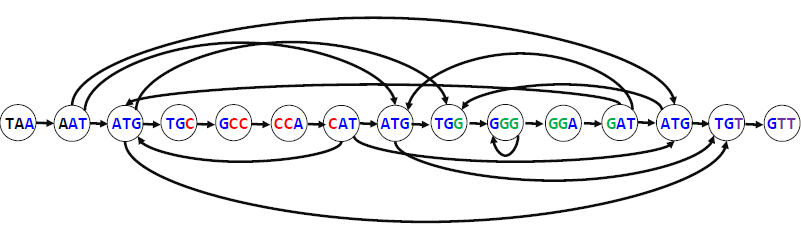
\includegraphics[width=1\textwidth]{poglavlja/3/slike/hamilton.png}
	\caption{Graf koji odgovara k-gramskom sastavu niske $TAATGCCATGGGATGTT$.}
	\label{slika:hamilton}
\end{figure} 

Jasno je da postoji više puteva u ovom grafu. Postavlja se pitanje, da li možemo da pronađemo genomsku putanju u ovom grafu, od svih koje postoje?

Podsetimo se šta je Hamiltonova putanja. Hamiltonova putanja je putanja koja posećuje svaki čvor u grafu tačno jednom. To je upravo ono što nam je potrebno za rešavanje problema. Svaki čvor predstavlja jedan k-gram i porebno nam je da svi k-grami budu uključeni u rekonstruisanu nisku tačno jednom.

\begin{problem}
	[Problem Hamiltonove putanje]
	Naći Hamiltonovu putanju u grafu.
	\\ Ulaz. Graf.
	\\Izlaz. Putanja koja posećuje svaki čvor u grafu tačno jednom.
\end{problem}

Iako deluje kao da smo rešili sve probleme, zapravo smo naišli na još jednu veliku prepreku. Naime, pronalaženje Hamiltonovog puta u grafu je NP-kompletan problem, što znači da ne postoji efikasan algoritam koji to radi.

U tom slučaju, moramo da se vratimo na početak, a to je predstavljanje k-gramskog sastava grafom.


\section{Rekonstrukcija niske kao Ojlerove putanje}


U prethodnoj sekciji k-grame smo predstavili čvorovima u grafu i u njemu tražili Hamiltonov put odnosno put koji obilazi svaki čvor tačno jednom. Videli smo da za taj problem još uvek nije poznat efikasan algoritam pa se sada pitamo kako možemo izmeniti graf tako da ne zahteva traženje Hamiltonove putanje.

Ono što se javlja kao ideja jeste obeležavanje grana umesto čvorova. Dakle, svaka grana biće obeležena jednim k-gramom, podniskama trih k-grama. Izlazni čvor biće obeležen prefiksom k-grama te grane, dok će ulazni čvor biti obeležen sufiksom istog tog k-grama. Na slici \ref{slika:ojler} ilustruje ovaj postupak za nisku $TAATGCCATGGGATGTT$.

\begin{figure}[H]
	\centering
	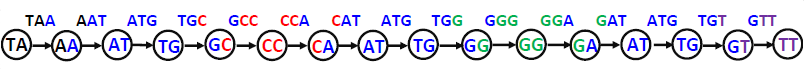
\includegraphics[width=1\textwidth]{poglavlja/3/slike/ojler.png}
	\caption{Graf koji odgovara 3-gramskom sastavu niske $TAATGCCATGGGATGTT$. Grane su obeležene 3-gramima, a čvorovi prefiksima/sufikisima.}
	\label{slika:ojler}
\end{figure} 


Primećujemo da su neki čvorovi obleženi identično (npr. imamo tri čvora sa oznakom $AT$). Sve čvorove koji imaju istu oznaku treba spojiti u jedan, pri čemu zadržavamo sve grane koje su ulazile u taj čvor ili su izlazile iz njega. Ponavljamo postupak dokle god imamo čvorove koji imaju istu oznaku i na kraju dobijamo graf koji nazivamo De Brojnov graf. 

\begin{figure}[H]
	\centering
	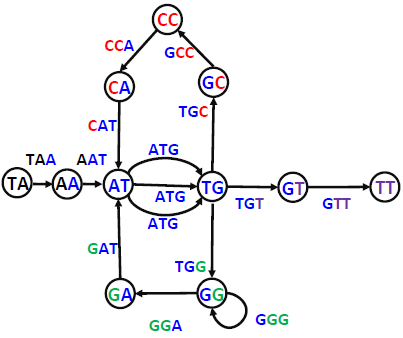
\includegraphics[width=0.6\textwidth]{poglavlja/3/slike/debrojnov.png}
	\caption{De Brojnov graf koji odgovara niski $TAATGCCATGGGATGTT$.}
	\label{slika:debrojnov}
\end{figure} 

Dobro, došli smo do nove reprezentacije niske pomoću grafa. Gde se sad nalazi naš \textit{Genome}? Kako nam se 3-grami sada nalaze na granama, a ne u čvorovima, potrebno je da pronađemo putanju u grafu koja prolazi sve grane tačno jednom. Takav put nazivamo \textit{Ojlerova putanja}. Srećom, algoritam za pronalaženje Ojlerove putanje u grafu nije NP-kompletan i možemo efikasno da je pronađemo.


\begin{problem}[Problem Ojlerove putanje]
	~\\ Pronaći Ojlerovu putanju u grafu.
	\\ Ulaz. Graf.
	\\ Izlaz. Putanja koja posećuje svaku granu u grafu tačno jednom.
\end{problem}


Sada znamo kako možemo da dobijemo nisku kada znamo de Brojnov graf koji odgovara njenom k-gramskom sastavu. Međutim, konstruisali smo de Brojnov graf na osnovu genoma, ali u realnim primenama, genom je nepoznat.


\section{De Brojnovi grafovi na osnovu kolekcije k-grama}

U redu, nije nam poznata niska, ali znamo njen k-gramski sastav. Za svaki k-gram pravimo dva čvora i jednu granu, na prethodno opisani način (\ref{slika:kgrami}).
Zatim lepimo identične čvorove sve dok ne dobijemo graf čiji svi čvorovi imaju različite oznake. Na slici je dat jedan korak ovog postupka, međutim tu nije kraj jer i dalje postoje čvorovi sa istim oznakama.

\begin{figure}[h]
	\centering
	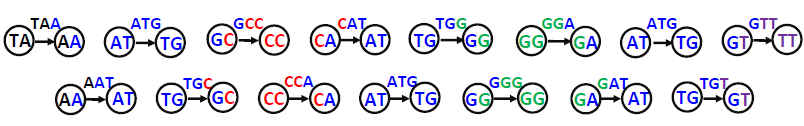
\includegraphics[width=1\textwidth]{poglavlja/3/slike/debrojnov1.png}
	\caption{Svaki k-gram prestavljen je pomoću dva čvora i jedne grane.}
	\label{slika:kgrami}
\end{figure} 

\begin{figure}[h]
	\centering
	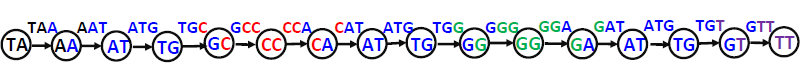
\includegraphics[width=1\textwidth]{poglavlja/3/slike/lepljenje.png}
	\caption{Postupak lepljenja čvorova. Posao nije završen!}
	\label{slika:lepljenje}
\end{figure} 


Po završetku postupka dobijamo de Brojnov graf koji je isti kao onaj koji smo dobili kada smo znali nisku. Svaka grana je označena jednim k-gramom. Svaki čvor je označen prefiksom/sufiksom izlazne/ulazne grane. Zalepljeni su svi čvorovi sa identičnim oznakama.

\section{Ojlerova teorema}

\begin{problem}[Problem Ojlerovog ciklusa]
	~\\ Pronaći ciklus Ojlerovom grafu.
	\\ Ulaz. Graf.
	\\ Izlaz. Ciklus koja posećuje svaku granu tačno jednom.
\end{problem}

\begin{teorema}[Ojlerova teorema]
	Svaki povezan graf i balansiran graf je Ojlerov.
\end{teorema}

Kažemo da je graf povezan ako za ma koja dva čvora postoji putanja koja ih povezuje.


%% MRAVI DOKAZUJU OJLEROVU TEOREMU

\begin{verbatim}
EulerianCycle(BalancedGraph)
form a Cycle by randomly walking in BalancedGraph (avoiding already visited edges)
while Cycle is not Eulerian
select a node newStart in Cycle with still unexplored outgoing edges
form a Cycle' by traversing Cycle from newStart and randomly walking afterwards
Cycle \leftarrow Cycle'
return Cycle
\end{verbatim}

\section{Sastavljanje parova očitavanja}

Od očitavanja do de Brojnovog grafa do genoma može se javiti više Ojlerovih putanja u grafu.

\subsection{DNK sekvenciranje sa parovima očitavanja} 

Imamo više identičnih kopija genoma i na slučajnim pozicijama sečemo genom na fragmente iste dužine \textit{InsertLength}. Zatim generišemo parove očitavanja: dva očitavanja sa krajeva svakog fragmenta na fiksiranoj udaljenosti.
Pod uparenim k-gramom podrazumevamo par k-grama na fiksiranom rastojanju d u genomu. Na primer, TCA i TCC na rastojanju d=11 čine jedan upareni k-gram.

\begin{problem} [Problem rekonstrukcije niske na osnovu parova očitavanja]
	~\\ Rekontruisati nisku na osnovu njenih uparenih k-grama.
	\\ Ulaz. Kolekcija uparenih k-grama.
	\\ Izlaz. Niska Text takva da je PairedComposition(Text) jednak kolekciji uparenih k-grama. 
\end{problem}

Kako konstruisati upareni de Brojnov graf na osnovu uparenog k-gramskog sastava?
Pretpostavimo da je dat genom (niska Genome). Posmatrajmo genom kao putanju u grafu obeleženom na osnovu njegovog uparenog kgramskog sastava.
\\
Pretpostavili smo da je dat genom (niska Genome). Posmatrali smo genom kao putanju u grafu obeleženom na osnovu njegovog uparenog k-gramskog sastava
\\
Sada pretpostavimo da nije dat genom već samo upareni k-gramski sastav

%% animacije, SVUDA ANIMACIJE!!!!!

~\\ Upareni de Brojnov graf na osnovu kolekcije uparenih k-grama:
\\ – Svaka grana je označena jednim uparenim k-gramom
\\ – Svaki čvor je označen prefiksima/sufiksima izlazne/ulazne grane
\\ – Zalepljeni su svi čvorovi sa identičnim oznakama.

\section{U realnosti}

Ovde smo imali neke nerealne pretpostavke.
\begin{itemize}
	\item  Savršena pokrivenost genoma očitavanjima (svaki k-gram iz genoma je očitan)
	\item Očitavanja ne sadrže greške
	\item Rastojanja između očitavanja u okviru parova očitavanja su egzaktna
	\item Nesavršena pokrivenost genoma očitavanjima (svaki k-gram iz genoma je očitan)
	\\ Očitavanja ne sadrže greške
	\\ Rastojanja između očitavanja u okviru parova očitavanja nisu egzaktna
\end{itemize}

\subsection{Savršena pokrivenost}

Prva nerealna pretpostavka je savršena pokrivenost.
\\
Očitavanja dužine 250 nukleotida dobijena Illumina tehnologijom predstavljaju samo mali deo 250-grama unutar genoma.
\\
Rešenje: razbiti dobijena očitavanja na kraće k-grame
\\
\\
Druga nerealna pretpostavka: očitavanja ne sadrže greške.

\newpage
\section{Zadaci sa vežbi}
U nastavku će biti predstavljeni zadaci sa vežbi na kursu rađeni u programskom jeziku Python.



\chapter{Kako sekvenciramo antibiotike?}
\setbookcodestyle


U ovom poglavlju i dalje govorimo o sekvenciranju, ali ćemo proširiti pogled i pokazati različite načine za sekvenciranje peptida. 

\section{Otkriće antibiotika} \label{otkrice}

Pre svega, krenućemo sa biološkim uvodom. Šta su to antibiotici? Sama reč antibiotik znači ,,onaj koji ubija život'', a tačnije, on predstavlja supstancu koja ubija bakterije. Kada ostavimo pomorandžu dugo negde gde je toplo, ona će da razvije čudne osobine kao što je buđ. Šta to znači? Buđ jeste jedna vrsta antibiotika što znači da se antibiotici nalaze u prirodi i da ih proizvode organizmi iz porodice gljiva (npr. buđi) i bakterija. 

Mi ćemo posmatrati antibiotike na molekularnom nivou koji nam govori od čega su oni zapravo izgrađeni. Od svih antibiotika posmatraćemo \textbf{\textit{tirocidin B1}}, antibiotik koji proizvodi bakterija \textit{Bacillus Brevis}. Tirocidin B1 na molekulskom nivou pripada \textit{peptidima}, kratkim niskama aminokiselina, odnosno malim proteinima. Ovo je skok u odnosu na ono što smo do sada posmatrali -- nukleotidne niske nad četvorostrukom azbukom $\Sigma = \{A, C, G, T\}$, odnosno DNK. Za DNK smo govorili da se pojavljuje u svakoj ćeliji svakog živog bića i da je veoma značajna supstanca jer sadrži recept (tačnije, nosi informaciju) za pravilno funkcionisanje i razvoj svakog živog bića. Da bi se svako živo biće pravilno razvijalo, neophodno je da njegove ćelije proizvode (sintetišu) u tačno određeno vreme određene supstance koje se nazivaju \textit{proteini}. DNK nosi informaciju o tome kako treba neki protein da izgleda, od čega treba da se sastoji. Zašto je to bitno? Na primer, kada je dan, neke biljke treba da vrše fotosintezu, a za vršenje fotosinteze treba u samim ćelijama biljaka da se sintetišu određeni proteini.

Proteini su, nakon nukleinskih kiselina, druga značajna grupa molekula koja sa računarske tačke gledišta takođe predstavlja dugačke niske, ali ne nad azbukom od 4 karaktera, nego nad azbukom od 20 karaktera, a svaki karakter predstavlja molekul koji se naziva \textit{aminokiselina}. Kao i nukleinske kiseline, aminokiseline se predstavljaju velikim latiničnim slovima $ \{V, K, L, F, P, W, N, Q, Y, G, A, I, M, D, E, S, T, C, R, H\}$, a pored toga postoje i troslovne oznake $\{Val, Lys, Leu, Phe, Pro, Trp, Asn, Gln, Tyr, Gly, Ala, Ile, Met, Asp, Glu, Ser, Thr, Cys, Arg, His\}$. U prirodi postoji mnogo više od 20 aminokiselina, ali 20 njih najčešće učestvuje u sastav proteina. DNK upravlja time kada će nastati protein u okviru ćelije. Recept za nastajanje svakog proteina je zapisan u DNK. Kako je taj recept zapisan, videćemo u nastavku.

Proteini se još nazivaju i \textit{polipeptidi}. Dužina proteina je obično od 100 aminokiselina do nekoliko hiljada (proteini su kraći od genomske sekvence). Tirocidin B1 je peptid jer se sastoji iz malog broja aminokiselina, svega deset -- $ V,K,L,F,P,W,F,N,Q,Y$. Problem sekvenciranja antibiotika jeste problem određivanja aminokiselina koje ulaze u sastav tog antibiotika. U prethodnom poglavlju smo sekvencirali genom, ali tehnike iz prethodnog poglavlja nećemo moći da koristimo u sekvenciranju tirocidina B1, što će biti objašnjeno u poglavlju \ref{pravljenje}.


\section{Kako bakterije prave antibiotike?} \label{pravljenje}

Pre rešavanja problema sekvenciranja antibiotika, govorićemo o zanimljivoj i kompleksnoj temi, a to je tema -- kako se prave proteini? Već je pomenuto da se u okviru DNK nalazi recept za pravljenje proteina. Sada je vreme da se zapitamo kako je sve to zapisano u DNK pomoću $A, C, G, T$.

Znamo da je DNK dvostruki lanac čiji su krajevi označeni sa 5' i 3' (uvek čitamo lanac od 5' ka 3'). DNK jeste jedna vrsta nukleinskih kiselina koje postoje u ćeliji živih bića. Pored nje, postoje i različite vrste \textbf{ribonukleinskih kiselinina}, odnosno \textbf{RNK}. Ribonukleinske kiseline nisu predstavljene dvostrukim lancem, već jednostrukim. One se sastoje od nukleotida $A, C, G, U$. Umesto timina, kod RNK se pojavljuje nukleotid uracil koji se označava sa $U$. 

DNK se \textbf{\textit{prepisuje}} u RNK. Šta to znači? Da bi nastali proteini, neophodno je da se na osnovu dva lanca od DNK konstruiše RNK molekul. Pošto se RNK molekul sastoji od istih nukleotida kao i DNK, osim timina, onda kažemo da formiranje RNK na osnovu DNK predstavlja jednostavno \textit{prepisivanje} nukleotida iz oba lanca DNK, uz zamenu nukleotida $T$ sa nukleotidom $U$. Drugi naziv za prepisivanje jeste \textit{transkripcija}. Ovo je prvi korak, i dalje nismo došli do aminokiseline, i dalje smo u azbuci nukleotida. RNK predstavlja jedan međukorak između DNK i samog proteina.

Drugi korak jeste \textit{prevođenje}, odnosno \textit{translacija}, prepisanog RNK u proteine. Imamo 4 nukleotida $A, C, G, U$ i treba njih da prevedemo u nisku od 20 mogućih aminokiselina. To znači da mora da postoji neko preslikavanje, nekakav kod koji prevodi neke $k$-grame nukleotida u aminokiseline. Nad azbukom od 4 nukleotida postoji 16 različitih $2$-grama, tj. bigrama. Da li možemo tih 16 bigrama da preslikamo u 20 aminokiselina? Tačnije, da li dva nukleotida možemo da preslikamo u jednu aminokiselinu? Ne možemo, jer moramo za svaku aminokiselinu da znamo koji je bigram označava. Pošto ne možemo to da uradimo sa bigramima, da li možemo sa $3$-gramima? Svih mogućih $3$-grama nad azbukom od 4 nukleotida ima 64. To znači da će svaka od aminokiselina imati svoj kod, a neke od njih će možda imati i više kodova, tj. više trigrama može da ukazuje na jednu aminokiselinu. To je u redu, bitno je da je naša funkcija ,,$na$'', ne mora da bude ,,$1-1$''. Ali kako napraviti funkciju? Ne možemo svojevoljno da dodelimo trigramima određene aminokiseline. Ta funkcija je unapred utvrđena, odnosno, prirodom determinisana i dokazana. U nastavku, koristićemo drugačiji naziv za naše $3$-grame. 
\\
\begin{definicija}
\textbf{Kodon} predstavlja jedan $3$-gram (triplet) nukleotida. \\
\end{definicija}

\noindent Preslikavanje o kojem je do sada bilo reči se naziva \textit{genetski kod} i on je prikazan na slici \ref{slika:genetskiKod}.
\\
\begin{definicija}
\textbf{Genetski kod} predstavlja preslikavanje skupa kodona u skup aminokiselina. \\
\end{definicija}


\begin{figure}[h!]
	\centering
	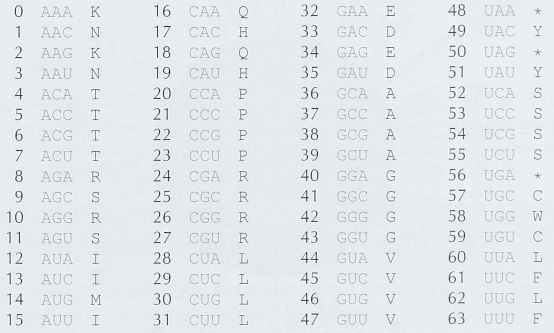
\includegraphics[width=0.8\textwidth]{poglavlja/4/slike/genetskiKod.png}
	\caption{Genetski kod.}
	\label{slika:genetskiKod}
\end{figure} 


Vidimo da se, na primer, kodon $UGG$ preslikava u aminokiselinu $Trp (W)$, dok se više kodona, $CUA, CUC, CUG, CUU, UUA, UUG$, preslikava u jednu aminokiselinu $Lys (L)$. 

Redom, kodone iz RNK preslikavamo u aminokiseline. Ali, kako znamo da je kraj nekog proteina? U genetskom kodu je i tako nešto kodirano. Postoje tzv. \textbf{stop kodoni} koji označavaju da iza njih nema više aminokiselina koje čine taj protein. Ti stop kodoni su $UAA, UAG, UGA$. 

\newpage


Dolazimo do jednog veoma značajnog biološkog aksioma -- \textbf{centralne dogme molekularne biologije}. Ona govori da se transkripcijom na osnovu DNK može dobiti RNK, a translacijom se iz RNK, na osnovu genetskog koda, dobijaju proteini. Ovu teoriju je predstavio Fransis Krik (eng. \textit{Francis Crick}) i prikazana je na slici \ref{slika:centralnaDogma}.
\begin{figure}[h!]
	\centering
	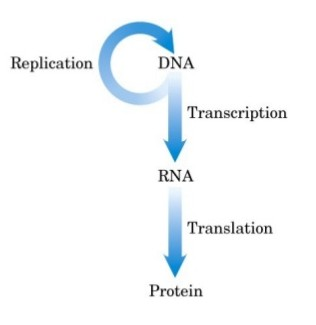
\includegraphics[width=0.5\textwidth]{poglavlja/4/slike/centralnaDog.jpg}
	\caption{Centralna dogma molekularne biologije.}
	\label{slika:centralnaDogma}
\end{figure} 



Ono što želimo da saznamo jeste koje aminokiseline i kojim redom ulaze u sastav našeg malog peptida tirocidina B1. Pošto se on sastoji iz 10 aminokiselina, to znači da ga čine 30 nukleotida u genomu bakterije \textit{Bacillus Brevis} koje će da se prepišu u RNK i da se prevedu iz RNK u tirocidin B1. Hiljade različitih $30$-grama se može prevesti u tirocidin B1 jer se u genetskom kodu različiti kodoni mogu prevesti u istu aminokiselinu. Na slici \ref{slika:30grami} su prikazani neki od takvih $30$-grama. Vidimo da oni nisu previše slični.
\begin{figure}[h!]
	\centering
	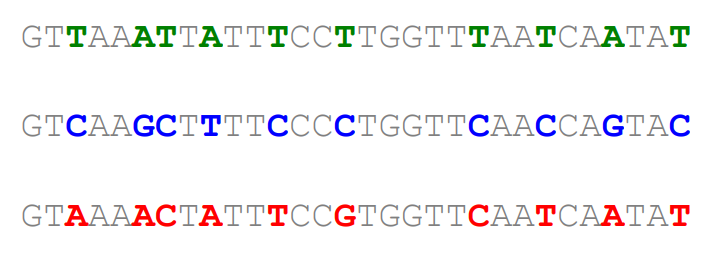
\includegraphics[width=0.8\textwidth]{poglavlja/4/slike/30grami.png}
	\caption{Neki od $30$-grama koji se mogu prevesti u tirocidin B1.}
	\label{slika:30grami}
\end{figure} 
\noindent

 Treba uzeti u obzir da translacija može početi na bilo kojoj poziciji u genomu. To znači da bismo za datu poziciju, ako gledamo $30$-gram, mogli da imamo 6 različitih tzv. \textbf{čitajućih okvira}, tj. 6 varijanti prepisivanja u RNK i onda prevođenja. Tri čitajuća okvira potiču iz tri nukleotida iz jednog kodona iz jednog prevedenog RNK lanca (ako krenemo da čitamo od prvog nukleotida, to je jedan čitajući okvir, iz drugog nukleotida je drugi čitajući okvir, iz trećeg nukleotida je treći čitajući okvir, a ako pročitamo od četvrtog nukleotida, to je već isti čitajući okvir kao prvi jer tu kreće novi kodon), a isto tako za drugi RNK lanac imamo tri čitajuća okvira sa druge strane. 

Naš peptid tirocidin B1 jeste \textit{cikličan}. Tih 10 aminokiselina koje ga čine idu nekim redom, ali su one povezane u krug, tako da imamo ukupno 10 različitih \textbf{linearnih reprezentacija} za tirocidin B1 u zavisnosti od toga koja nam je prva aminokiselina bila u samom receptu DNK. Koju god linearnu reprezentaciju pronađemo, rešili smo problem. 
\\\\
\indent Ne odustajemo od pronalaženja $30$-grama u genomu bakterije \textit{Bacillus Brevis} koji kodira bar jednu linearnu reprezentaciju od svih 10 koje čine tirocidin B1. Pretpostavimo da imamo na raspolaganju veoma moćan računar i neograničeno vreme. Doći ćemo do jednog čudnog rezultata. Nećemo uspeti da pronađemo nijedan $30$-gram u genomu bakterije \textit{Bacillus Brevis} koji kodira bar jednu linearnu reprezentaciju proteina tirocidina B1. Zašto? Stvari se komplikuju. Na ovom primeru je pokazano da centralna dogma ne važi uvek, odnosno ne važi da svaki protein u ćeliji nastaje na osnovu recepta koji je zapisan u DNK. Centralna dogma govori da se proces transkripcije izvršava pod uticajem enzima koji se zove \textit{RNK polimeraza}, a translacija RNK u protein se vrši u ćelijskoj organeli koja se naziva \textit{ribozom}. Postoje neki proteini koji ne nastaju na ovaj način, nego na specijalan način gde obično sekvenciranje genoma ne može da nam pomogne. Moramo da predložimo novi metod kako možemo da pronađemo odgovarajuću sekvencu aminokiselina. 

Edvard Tejtum (eng. \textit{Edward Tatum}), jedan od poznatih američkih genetičara, je 1963. godine inhibirao ribozom bakterije \textit{Bacillus Brevis}. Šta ovo znači? S obzirom da se znalo da se u ribozomu vrši translacija RNK u protein, on je onemogućio da se bilo šta desi u ribozomu, isključio je funkcionisanje te organele u ćeliji i očekivao je da se neće stvoriti nijedan protein, pa ni tirocidin B1. Međutim, suprotno očekivanjima, nastavljena je proizvodnja nekih peptida, uključujući i tirocidine. Ovo je bilo izuzetno iznenađujuće otkriće.

Fric Lipman (eng. \textit{Fritz Lipmann}), američko-nemački biohemičar, je 1969. godine  pokazao da tirocidini spadaju u grupu \textbf{ne-ribozomalnih peptida (NRP-ova)}. To su peptidi za čiju sintezu nisu odgovorni ribozomi i RNK polimeraza već enzimi poznati pod nazivom \textbf{NRP sintetaze}, molekuli koji se takođe nalaze u ćeliji i utiču na različite procese koji se dešavaju u njoj. To znači da se stvaranje tirocidina razlikuje od većeg broja proteina u živim bićima. 
\\\\
\indent Kako izgleda sinteza tirocidina B1 pomoću NRP sintetaze? Postoji veliki broj različitih NRP sintetaza, nije samo jedna odgovorna za stvaranje svih mogućih NRP-ova, nego za svaki ne-ribozomalni peptid postoji odgovarajuća NRP sintetaza. Ona NRP sintetaza koja je odgovorna za stvaranje tirocidina B1 se sastoji od 10 različitih podjedinica koje nazivamo \textit{moduli}. Svaki modul je odgovoran za nadovezivanje jedne aminokiseline na budući molekul tirocidina B1. Svaki od modula privuče jednu aminokiselinu i spoji je sa prethodnom, a poslednji korak jeste cirkularizacija -- spajanje aminokiselina nastalih uz pomoć prvog i poslednjeg modula radi kreiranja cikličnog peptida.

\section{Sekvenciranje antibiotika razbijanjem na komade} \label{razbijanje}

Pošto nam sekvenciranje genomske sekvence i pronalaženje odgovarajuće podniske koja je zadužena za translaciju u aminokiseline odgovarajućeg peptida ne može pomoći u sekvenciranju tirocidina B1 (jer on ne nastaje na osnovu informacije zapisane u DNK), postavljamo pitanje da li postoji način na koji možemo da sekvenciramo antibiotike. Moramo direktno da sekvenciramo peptid. Jedan od načina jeste \textbf{sekvenciranje razbijanjem na komade} i biće predstavljen u ovoj sekciji.
\\\\

\indent U sekvenciranju antibiotika može nam pomoći mašina koja se naziva \textbf{maseni spektrometar} i koju možemo opisati kao skupu molekularnu vagu. Šta on radi? Za početak ćemo da se zapitamo kako možemo da merimo težinu, tačnije masu molekula. 

Pošto se molekuli sastoje od atoma, prvo treba da govorimo o masi pojedinačnog atoma. U atomima postoje protoni, neutroni i elektroni. Protoni i neutroni su približno iste mase, dok su elektroni izuzetno mali i gotovo zanemarljive mase. Zato masu jednog atoma možemo svesti na masu protona, odnosno neutrona koji učestvuju u izgradnji konkretnog atoma koji posmatramo, pa se i masa molekula može izračunati kao suma masa atoma koji ga čine. Maseni spektrometar vraća masu molekula izračunatu u \textbf{Daltonima}. 
\begin{center}
$1 \quad Dalton (Da) \approx masa \quad jednog \quad protona/neutrona$ \\
$Masa \quad molekula \approx suma \quad masa \quad protona/neutrona$
\end{center}

Posmatrajmo masu jedne aminokiseline, recimo glicina. Glicin ima hemijsku formulu $ C_{2}H_{3}ON $. Ugljenik ima masu 12, vodonik ima masu 1, kiseonik 16, a azot 14. Na osnovu ovih masa računamo masu celog molekula glicina.
\begin{center}
$  masa(C_{2}H_{3}ON) = 12*2 + 1*3 + 16*1 + 14*1 \approx 57 Da $
\end{center}

\noindent Simbol  $ \approx $ koristimo jer nam je stvarna masa nešto malo drugačija od celobrojne mase koju dobijamo ovde. Stvarna masa glicina iznosi $ 57.02 Da $. Podrazumevaćemo da je masa celog molekula upravo celobrojna masa koju smo dobili.

Tabela masa svih aminokiselina data je u tabeli \ref{tabela:mase}.

\begin{center}
\begin{table} [h!]
\centering
\caption{Tabela masa 20 aminokiselina poređanih rastuće prema celobrojnim masama.}
\label{tabela:mase}
\begin{tabular}{ |c|c|c|c|c|c|c|c|c|c|c|c|c|c|c|c|c|c|c|c| } 
 \hline
 G & A & S & P & V & T & C & I,L & N &  D & K,Q & E & M & H & F & R & Y & W\\ 
 \hline 
 57 & 71 & 87 & 97 & 99 & 101 & 103 & 113 & 114 & 115 & 128 & 129 & 131 & 137 & 147 & 156 & 163 & 186 \\ 
 \hline
\end{tabular}
\end{table}
\end{center}

Primećujemo da neke aminokiseline imaju iste mase, npr. $I$ i $L$, $K$ i $Q$, pa za 20 aminokiselina imamo 18 celobrojnih masa.

Kada imamo mase aminokiselina, možemo da se zapitamo koja je masa tirocidina B1. Znajući da se tirocidin B1 sastoji iz 10 aminokiselina ovim redom: $ VKLFPWFNQY $, masu računamo koristeći tabelu \ref{tabela:mase}. 

\begin{center}
$  masa(tirocidina \quad B1) = 99+128+113+147+97+186+147+114+128+163 = 1322 $
\end{center}

Vratimo se na maseni spektrometar o kojem smo govorili ranije. Zamislimo da imamo kratak peptid koji se sastoji od samo 4 aminokiseline $NQEL$. Uzorak ovog peptida ubacimo u maseni spektrometar. Šta se u njemu dešava? U njemu se nekim hemijskim procesima, u čije detalje nećemo ulaziti, generišu svi podpeptidi ulaznog peptida. Sa računarske tačke gledišta, maseni spektrometar generiše od zadate niske $NQEL$ sve moguće podniske, podrazumevajući da je ulazni peptid cikličan. Tako se generišu podniske dužine jedan: $N, Q, E, L$, podniske dužine dva: $NQ, QE, EL, LN$ i podniske dužine tri: $NQE$, $QEL$, $ELN$, $LNQ$. Maseni spektrometar za svaki od dobijenih podpeptida može da odredi molekulsku masu. Ono što mi dobijemo kao izlaz iz masenog spektrometra nisu podpeptidi, mi ne znamo koje podpeptide je dobio, niti kojim podpeptidima je prudružena koja masa. Izlaz iz masenog spektrometra jeste samo niz masa! Taj izlazni niz može da sadrži i dva ista broja jer neki podpeptidi mogu da imaju istu masu.

Kako bismo formulisali računarski problem, moramo da definišemo šta je to \textit{teorijski spektar}. 
\begin{definicija} \textbf{Teorijski spektar peptida} predstavlja niz masa svih mogućih podpeptida tog peptida, uključujući nulu kao masu praznog peptida i masu samog peptida.
\end{definicija}

Poznajući sastav peptida, lako možemo da izračunamo teorijski spektar. Suprotan smer je težak, odnosno teško je da na osnovu teorijskog spektra zaključimo kako je izgledao peptid. Upravo ovo jeste problem sekvenciranja ciklopeptida.

\begin{problem}[Problem sekvenciranja ciklopeptida] 
	Rekonstruisati ciklični peptid na osnovu njegovog teorijskog spektra. \\
\end{problem}



\subsection{Sekvenciranje ciklopeptida grubom silom}

Kada dobijemo spektar iz masenog spektrometra, najveća masa će označavati masu celog peptida. Želimo prvo da generišemo sve peptide sa masom jednakom masi celog peptida, zatim da za svaki tako generisan peptid formiramo teorijski spektar i uporedimo ga sa datim spektrom. Algoritam grube sile za problem sekvenciranje ciklopeptida dat je u nastavku. 

\begin{lstlisting}
BFCyclopeptideSequencing(Spectrum)
begin
	// ParentMass(Spectrum) jeste najveca masa u spektru Spectrum
	for every Peptide with Mass(Peptide) equal to ParentMass(Spectrum)
		if Spectrum == CycloSpectrum(Peptide)
			output Peptide
end
\end{lstlisting}

Vidimo da u ovom algoritmu ispitujemo sve kandidate (peptide sa istom masom kao dati peptid). Koliko imamo takvih kandidata? Grafik koji oslikava odgovor na ovo pitanje dat je na slici \ref{slika:kolikoPeptida}.

\begin{figure}[h!]
	\centering
	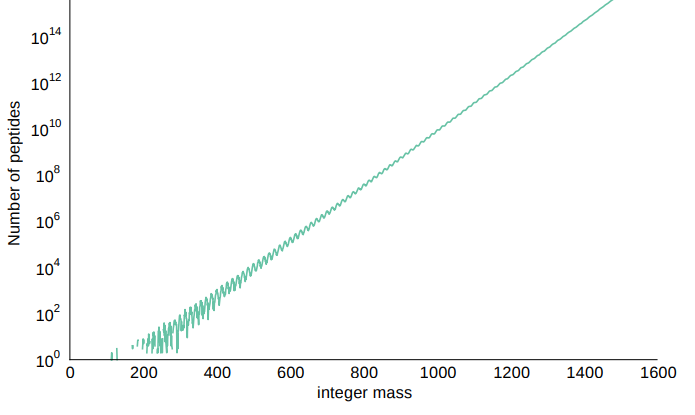
\includegraphics[width=0.7\textwidth]{poglavlja/4/slike/kolikoPeptida.png}
	\caption{Broj peptida sa zadatom masom.}
	\label{slika:kolikoPeptida}
\end{figure} 


Vidimo da je ovaj algoritam grube sile eksponencijalne složenosti. Pod uslovom da imamo dovoljno brz računar, ovako nešto bismo i mogli da izračunamo. Ali, šta bi bili nedostaci ovog algoritma grube sile? Možemo da imamo dva peptida sa istom masom, a da su potpuno različiti. Na primer, peptid $NQEL$ i peptid $TMDH$ imaju masu 484. Kako možemo da isključimo pogrešan peptid? Za oba ova peptida možemo da generišemo teorijski spektar. Ispostavlja se da su njihovi spektri potpuno različiti. Želimo da ovu informaciju iskoristimo u sledećem pristupu rešavanja problema sekvenciranja ciklopeptida. Cilj nam je da ne idemo grubom silom već da ogroman broj kandidata od samog početka odstranimo.
\newpage

\subsection{\textit{Branch-and-Bound} algoritam za sekvenciranje ciklopeptida}

U ovom pristupu postepeno konstruišemo kandidate za rešenja od manjih linearnih peptida za razliku od prethodnog pristupa u kome smo odmah generisali ceo peptid koji postaje kandidat. Na taj način ćemo smanjiti ukupan broj linearnih peptida koje posmatramo. Ovakav pristup se koristi kod \textbf{\textit{Branch-and-Bound} algoritama} koji će biti opisani u nastavku.

Kod \textit{Branch-and-Bound} algoritama u celokupnom prostoru svih mogućih rešenja vršimo nekakva odsecanja. Počnemo od kratkog peptida dužine jedan, pa ga proširimo na sve moguće načine, odnosno, dodamo po jednu aminokiselinu i od toga napravimo sve moguće kandidate dužine dva. To je \textit{branch grana} i predstavljena je na slici \ref{slika:branch}. \textit{Bound grana} bi od postojećih kandidata, nastalih u \textit{branch} granama, isključila neke potencijalne kandidate. \textit{Bound} grana je predstavljena na slici \ref{slika:bound}. Postupak proširivanja i odsecanja ponavljamo sve dok ne dođemo do odgovarajućih vrednosti. Na ovaj način će nam ostati mnogo manje kandidata za rešenja nego u prethodnom pristupu grube sile.

\begin{minipage}{\textwidth}
	\centering
	\begin{minipage}{0.45\textwidth}
		\begin{figure}[H]
			\centering
			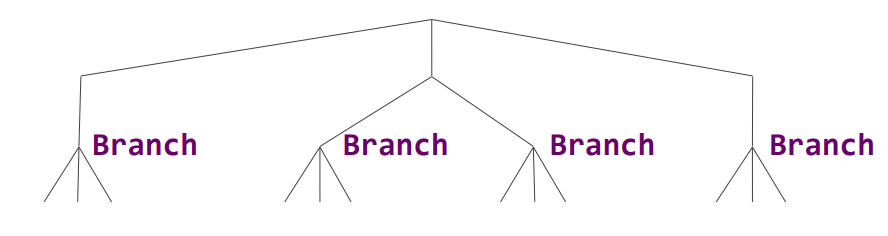
\includegraphics[width=\textwidth]{poglavlja/4/slike/branch.png}
			\caption{\textit{Branch} grane algoritma \textit{Branch-and-Bound}.}
			\label{slika:branch}
		\end{figure} 
	\end{minipage}
	\hfill 
	\begin{minipage}{0.45\textwidth}
		\begin{figure}[H]
			\centering
			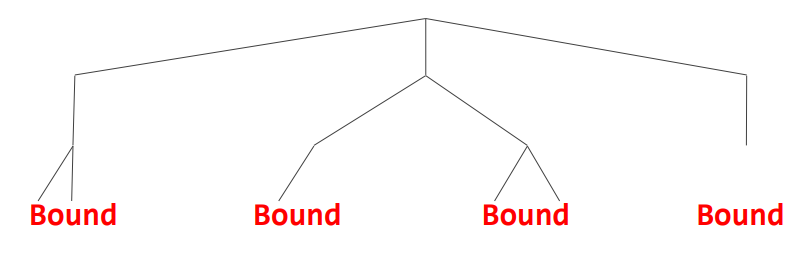
\includegraphics[width=\textwidth]{poglavlja/4/slike/bound.png}
			\caption{\textit{Bound} grane algoritma \textit{Branch-and-Bound}.}
			\label{slika:bound}
		\end{figure} 
	\end{minipage}
	\vspace*{1em}
\end{minipage}

Primenimo ovaj algoritam na konkretan problem. Recimo da nam je dat spektar
\begin{center}
 0 97 97 99 101 103 196 198 198 200 202 295 297 299 299 301 394 396 398 400 400 497.
 \end{center} 
\noindent  Vidimo da se u datom spektru nalaze mase nekih aminokiselina, što nam govori koje aminokiseline ulaze u sastav traženog peptida. Te aminokiseline su $P,V,T,C$ sa masama $97,99, 101, 103$. Ovo znači da možemo da počnemo ne sa svih 20 aminokiselina, nego sa 4 unigrama $P,V,T,C$. Ovo je unapred jedna \textit{bound} grana jer smo 20 aminokiselina sveli na 4 kandidata aminokiselina. Zatim idemo na branch granu, širimo unigrame u sve moguće bigrame: $PA$, $PC$, $PD$,..$PY$, $VA$, $VC$, $VD$,...,$VY$, $TA$, $TC$, $TD$,..., $TY$, $CA$, $CC$, $CD$,..., $CY$. Proširujemo sa svih 20 aminokiselina jer ćemo kasniji videti da ovako zadati spektar jeste čisto teorijski spektar, a maseni spektrometar skoro nikada u praksi ne vraća teorijski spektar već spektar sa nekakvim greškama. Kako možemo da skratimo ovu listu, kako možemo da izvršimo korak \textit{bound} u ovom trenutku? Posmatramo da li postoje odgovarajući bigrami koji se takođe pojavljuju u spektru. Zbog toga uvodimo pojam \textbf{konzistentnosti}.

\begin{definicija}
Za proizvoljan podpeptid $p_{1},..,p_{n}$ kažemo da je \textbf{konzistentan} sa spektrom $S$ ukoliko se svaka masa iz teorijskog spektra podpeptida  $p_{1},..,p_{n}$ nalazi u spektru $S$.
\end{definicija}

Na primer, $PV$ je \textbf{konzistentno} sa spektrom ukoliko se masa od $P$, masa od $V$ i masa od $PV$ nalaze u spektru.

Konzistentnost ćemo koristiti u \textit{bound} koraku, tačnije, izbacićemo sve bigrame koji nisu konzistentni sa spektrom. Tako dobijemo listu konzistentnih bigrama $PV$, $PT$, $PC$, $VP$, $VT$, $VC$, $TP$, $TV$, $CP$, $CV$ koju proširujemo u sve moguće $3$-grame, a zatim svodimo na listu samo konzistentnih $3$-grama. Postupak ponavljamo. Kada dođemo do liste konzistentnih pentagrama $PVCPT$, $PTPVC$, $PTPVC$, $PCVPT$, $VPTPC$, $VCPTP$, $TPVCP$, $TPCVP$, $CPTPV$, $CVPTP$ vidimo da zapravo svi oni pokazuju na jedan isti ciklični peptid.

Pseudokod opisanog algoritma dat je u nastavku.
\begin{lstlisting}
CyclopeptideSequencing(Spectrum)
begin
	Peptides = a set containing only the empty peptide
	while Peptides is non-empty
		// prosirujemo sve peptide u skupu sa svim mogucim aminokiselinama
		Peptides = Expand(Peptides)
		for each Peptide in Peptides
			// ParentMass(Spectrum) jeste najveca masa u spektru
			if Mass(Peptide) = ParentMass(Spectrum)
				if Cyclospectrum(Peptide) = Spectrum
					output Peptide
				remove Peptide from Peptides
			else if Peptide is not consistent with Spectrum
				remove Peptide from Peptides
end
\end{lstlisting}

Podsetimo se da je složenost algoritma grube sile, koji ovde pokušavamo da poboljšamo, eksponencijalna. Ispostavlja se da \textit{Branch-and-Bound} algoritam takođe može biti eksponencijalne složenosti za neke peptide, ali je u praksi veoma brz.



\section{Prilagođavanje sekvenciranja za spektre sa greškama} \label{greskeSpektri}

Spektar koji smo do sada definisali jeste teorijski spektar. Za razliku od njega, spektar koji izlazi iz masenog spektrometra, \textbf{eksperimentalni spektar}, često sadrže greške. O kakvim greškama se govori biće prikazano pomoću slike \ref{slika:ekspSpektar}.

\begin{figure}[h!]
	\centering
	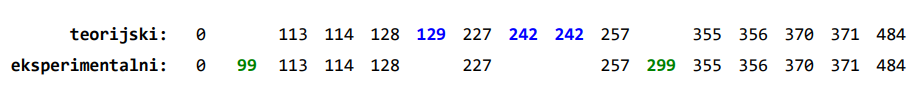
\includegraphics[width=0.9\textwidth]{poglavlja/4/slike/ekspSpektar.png}
	\caption{Primer teorijskog i eksperimentalnog spektra za $NQEL$.}
	\label{slika:ekspSpektar}
\end{figure} 

\textbf{Lažne mase} jesu mase koje su na slici \ref{slika:ekspSpektar} prikazane zelenom bojom. To su mase koje su prisutne u eksperimentalnom spektru, ali nisu prisutne u teorijskom spektru.

\textbf{Nedostajuće mase} jesu mase koje su na slici \ref{slika:ekspSpektar} prikazane plavom bojom. To su mase koje se nalaze u okviru teorijskog spektra, ali ne i u okviru eksperimentalnog spektra.

Zbog pojave ovih otežavajućih okolnosti, tj. grešaka u spektru, neophodan je novi algoritam jer se kod dva predložena algoritma teorijski spektar peptida morao u potpunosti poklapati sa spektrom peptida koji je predstavljao rešenje problema. Sada moramo da olabavimo taj uslov pa uvodimo pojam \textbf{skor peptida}.

\begin{definicija}
\textbf{Skor peptida} pokazuje koliko masa njegov teorijski spektar deli sa eksperimentalnim spektrom.
\end{definicija}

\noindent Tako, za sliku \ref{slika:ekspSpektar}, skor iznosi 11. Želimo da skor bude što veći.

S obzirom da imamo nov način upoređivanja, moramo da unapredimo naš \textit{Branch-and-Bound} algoritam, konkretno korak odsecanja. 

Uzmimo primer golfa. U golfu, kada igrači prođu prvi krug takmičenja, u sledeći krug prolaze dalje samo igrači koji su konkurentni, oni koji imaju šanse da nešto osvoje. To znači da možemo da kažemo da nam je odsecanje takvo da, na primer, prva tri igrača sa najboljim skorom idu dalje, a ukoliko imamo još neke igrače koji imaju isti skor kao poslednji igrač, onda i oni prolaze dalje. Znači, zadržavaju se tri najbolja igrača \textit{,,with ties''}. Ovakav sistem primenjen na \textit{Branch-and-Bound} algoritam prikazan je u sledećem pseudokodu.

\begin{lstlisting}
LeaderboardCyclopeptideSequencing(Spectrum, N)
begin
	Leaderboard = set containing only the empty peptide
	LeaderPeptide = empty peptide
	
	while Leaderboard is non-empty
		// prosirujemo sve elemente koji se nalaze u okviru skupa Leaderboard
		Leaderboard = Expand(Leaderboard)
		for each Peptide in Leaderboard
			// ParentMass(Spectrum) predstavlja najvecu masu u spektru Spectrum
			if Mass(Peptide) == ParentMass(Spectrum)
				if Score(Peptide, Spectrum) > Score(LeaderPeptide, Spectrum)
					LeaderPeptide = Peptide
			else if Mass(Peptide) > ParentMass(Spectrum)
				remove Peptide from Leaderboard
		// odsecamo kandidate iz Leaderboard na osnovu njihovog skora
		Leaderboard = Trim(Leaderboard, Spectrum, N)
		
	output LeaderPeptide
end

Trim(Leaderboard, Spectrum, N, AminoAcid, AminoAcidMass)
begin
	for j=1 to |Leaderboard|
		Peptide = j-th peptide in Leaderboard
		// LinearScore jeste skor nad linearnim spektrom
		LinearScores[j] = LinearScore(Peptide, Spectrum)
		
	sort Leaderboard according to the dec order of scores in LinearScores
	sort LinearScores in dec order
	
	for j=N+1 to |Leaderboard|
		if LinearScores[j] < LinearScores[N]
			remove all peptides starting from the j-th peptide from Leaderboard
			return Leaderboard
			
	return Leaderboard
end
\end{lstlisting}

\noindent \textit{Leaderboard} pristup omogućava da bolje definišemo za esperimentalni spektar kod \textit{Branch-and-Bound} algoritma onu bound fazu kada treba da izbacimo neke kandidate. 

\subsection{Testiranje na spektru tirocidina B1}

U ovom delu razmatraćemo rezultate testiranja na $Spectrum_{10}$, spektru sa 10\% lažnih/nedostajućih masa. 

Kada primenimo \textit{LeaderboardCyclopeptideSequencing} na spektar sa 10\% loših vrednosti, tada zaista dobijemo peptid sa najvišim skorom $ VKLFPWFNQY $  koji odgovara tirocidinu B1. Međutim, ukoliko uzmemo spektar $Spectrum_{25}$ koji ima 25\% lažnih i nedostajućih vrednosti, spektar koji se još više udaljava od teorijskog spektra, onda se peptid sa najvišim skorom $ VKLFPADFNQY $ razlikuje od peptida  $ VKLFPWFNQY $ koji želimo da dobijemo.

Ovo znači da \textit{LeaderboardCyclopeptideSequencing} algoritam radi dobro kada nam je eksperimentalni spektar malo različit od teorijskog.

\section{Od 20 do više od 100 aminokiselina} \label{viseAmino}

U ovoj sekciji biće reči o poboljšanju našeg algoritma uz uvođenje premisa koje postoje u stvarnosti, a koje smo do sada zanemarivali da bismo dali neke početne načine za rešavanje.

Kada smo govorili o proteinima, rekli smo da 20 aminokiselina najčešće učestvuje u njihovoj izgradnji i da su za nas, sa računarske tačke gledišta, proteini niske nad azbukom od 20 karaktera i da postoji još veliki broj aminokiselina nezavisno od izgradnje proteina u ćelijama živih bića. U gentskom kodu postoje kodovi samo za tih 20 aminokiselina, i u tabeli celobrojnih masa aminokiselina postoje mase samo za iste te aminokiseline. S obzirom da u ovom poglavlju razmatramo NRP peptide, peptide koji ne nastaju prema pravilima centralne dogme,  onda ovi peptidi mogu da sadrže i neke nestandardne aminokiseline, one aminokiseline koje se ne nalaze među standardnih 20 aminokiselina. Na primer, tirocidin B sadrži nestandardnu aminokiselinu \textit{Ornitin (Orn)}. Za Ornitin ne postoji nukleotidni triplet u okviru genetskog koda na osnovu koga se ova aminokiselina dobija i ne postoji celobrojna masa u tabeli celobrojnih masa za aminokiseline. S ozbirom na to, možemo da pretpostavimo da bilo koji ceo broj između 57 i 200 (koliko nam iznosi najmanja i najveća masa standardnih aminokiselina) može biti masa neke nestandardne aminokiseline. Ovako nešto može da izgleda kao grubo ograničenje, ali je eksperimentalno potvrđeno da većina masa svih mogućih aminokiselina pripada ovom intervalu.

Spektar u kome nismo ograničeni na tabelu od samo 18 celobrojnih masa, već uzimamo u obzir da bilo koji celi broj između 57 i 200 može da označava neku aminokiselinu, nazivamo \textbf{prošireni spektar}. Kada primenimo Leaderboard algoritam na prošireni spektar sa 10\% lažnih i nedostajućih masa, peptid koji dobijemo $  VKLFPWFN-98-65 $ sadrži neke vrednosti za mase koje ne odgovaraju nijednoj aminokiselini. Pošto Leaderboard algoritam ovde ne daje ispravne vrednosti, moramo da primenimo jedan sasvim novi princip.

\section{Spektralna konvolucija} \label{konvolucija}

Kod algoritma sa proširenim spektrom podrazumeva se da svi celi brojevi između 57 i 200 odgovaraju masama aminokiselina. To znači da razmatramo 144 ili više (znamo da jednoj masi može da odgovara više aminokiselina, a sa druge strane postoje vrednosti kojima ne odgovara nijedna) aminokiselina u koje spadaju i standardne i nestandardne aminokiseline. Želimo da smanjimo broj aminokiselina koje razmatramo. 

Posmatrajmo eksperimentalni spektar za $ NQEL $
\begin{center}
0 99 113 114 128 227 257 299 355 356 370 371 484.
\end{center}
\noindent Mi znamo da je $ Mass(E) = 129 $ i vidimo da u spektru ne postoji ta vrednost. Sa druge strane, u spektru postoji $ Mass(QE) = 257 $ i $ Mass(Q) = 128 $. Razlika ove dve mase daje vrednost $129$. Ova vrednost već deluje kao dobra vrednost za nedostajuću masu. U spektru postoji još ovakvih slučajeva. Recimo, $ Mass(ELN) - Mass(LN) = 356 - 227 = 129 $ i $ Mass(NQEL) - Mass(LNQ) = 484 - 355 = 129 $. Obe ove razlike ukazuju na masu od $E$ koja nedostaje.

Uvodimo tabelu koja se naziva \textbf{spektralna konvolucija}.
\begin{definicija}
\textbf{Spektralna konvolucija} je tabela koja pokazuje apsolutnu vrednost razlike između svake dve mase u spektru.
\end{definicija}

Primer spektralne konvolucije za spektar čije su lažne vrednosti označene sa ,,false'' prikazan je na slici \ref{slika:spektralnaKonvolucija}.

\begin{figure}[h!]
	\centering
	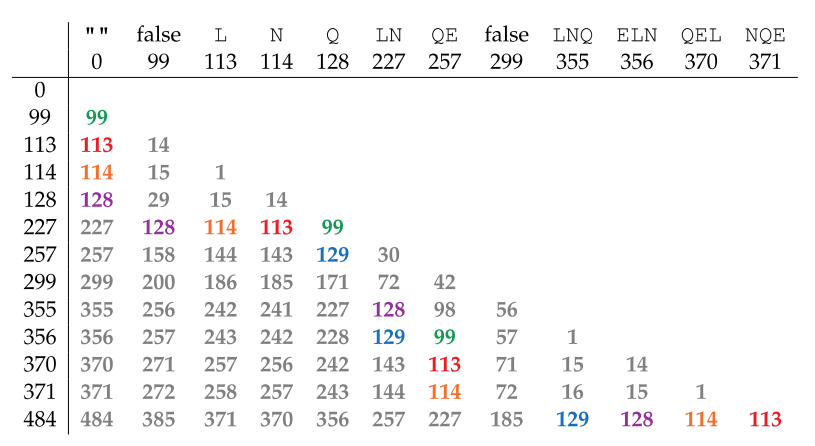
\includegraphics[width=0.9\textwidth]{poglavlja/4/slike/spektralnaKonvolucija.png}
	\caption{Primer spektralne konvolucije.}
	\label{slika:spektralnaKonvolucija}
\end{figure}

\noindent Na preseku svake vrste i kolone u spektralnoj konvoluciji upisana je apsolutna vrednost razlike celobrojnih masa. Kako iskoristiti spektralnu konvoluciju? Tražimo vrednosti razlika koje se pojavljuju najveći broj puta, a da se nalaze između 57 i 200. Obojene vrednosti na slici \ref{slika:spektralnaKonvolucija} se pojavljuju veći broj puta. To su vrednosti 99, 113, 114, 128 i 129. Ove vrednosti odgovaraju masama aminokiselina, redom, $V, L, N, Q, E $. Od 5 najčešćih aminokiselina u konvoluciji 4 čine peptid $NQEL$.

Kako bi izgledao unapređeni algoritam za sekvenciranje ciklopeptida ukoliko uzmemo u obzir i nestandardne aminokiseline, odnosno proširenu tabelu celobrojnih masa aminokiselina? Pseudokod je dat u nastavku.
\begin{lstlisting}
ConvolutionCyclopeptideSequencing(Spectrum, N, M)
begin
	Formirati spektralnu konvoluciju spektra Spectrum.
	Uzeti M najcescih elemenata u konvoluciji (izmedju 57 i 200).
	Primeniti LeaderboardCyclopeptideSequencing, formirajuci peptide samo na osnovu ovih M celih brojeva.
end
\end{lstlisting}

Algoritam  \textit{ConvolutionCyclopeptideSequencing} daje tačan rezultat i za spektre sa šumom od 10\% i za spektre sa šumom od 25\%, što pokazuje da je spektralna konvolucija odgovorila na sve izazove koji su postavljeni.

\section{Spektri u realnosti} \label{realnost}

Kao što znamo, realnost je obično drugačija. Neke poteškoće iz realnosti smo zanemarivali. Koje?
\begin{itemize}
	\item $Spectrum_{25}$ je mnogo manje šumovit nego spektri dobijeni u praksi iz masenog spektrometra.
	
	\item Maseni spektrometar ne meri jednostavno fragmente podpeptida, već su postupci merenja mnogo komplikovaniji. Najpre se zaista vrši razbijanje datog peptida na fragmente. Zatim se oni sortiraju, korišćenjem elektromagnetnog polja, prema svojoj masi. Ono što maseni spektrometar meri jeste zapravo \textbf{odnos mase i naelektrisanja} za svaki fragment (znači nije baš masa) i određuje \textbf{intenzitet} (kao broj jona) u svakom odnosu mase i naelektrisanja. Šta to znači? To znači da kao izlaz iz masenog spektrometra ne dobijamo eksperimentalni spektar koji smo do sada imali prilike da vidimo, nego grafik intenziteta prema odnosu mase i naelektrisanja sa vrhovima na određenim mestima. Primer ovakvog grafika dat je na slici \ref{slika:intenzitet}.
	\begin{figure}[h!]
	\centering
	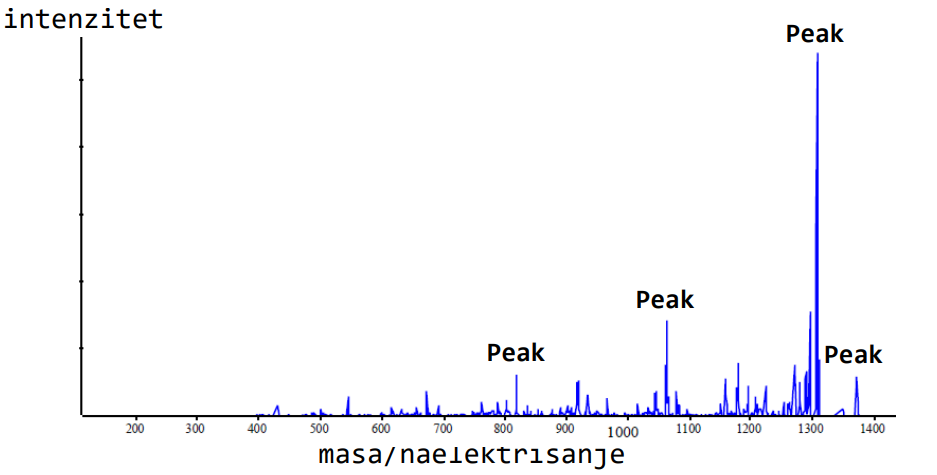
\includegraphics[width=0.9\textwidth]{poglavlja/4/slike/intenzitet.png}
	\caption{Primer grafika intenziteta prema odnosu mase i naelektrisanja.}
	\label{slika:intenzitet}
\end{figure}
	Na osnovu vrhova na grafiku, određivaćemo sam sastav peptida. Ovaj grafik se naziva \textbf{realni spektar}. Rekonstrukcija peptida na osnovu realnog spektra biće obrađena u poglavlju 11.
	
\end{itemize}

\newpage
\section{Zadaci sa vežbi}
\setexamplecodestyle

U nastavku će biti predstavljeni zadaci sa vežbi na kursu rađeni u programskom jeziku Python.

\subsection{Linear Spectrum}

\lstinputlisting[language=Python]{poglavlja/4/kodovi/LinearSpectrum.py}

\subsection{Cyclic Spectrum}

\lstinputlisting[language=Python]{poglavlja/4/kodovi/CyclicSpectrum.py}

\subsection{Cyclopeptide Sequencing}

\lstinputlisting[language=Python]{poglavlja/4/kodovi/CyclopeptideSequencing.py}

\subsection{Leaderboard Cyclopeptide Sequencing}

\lstinputlisting[language=Python]{poglavlja/4/kodovi/LeaderboardCyclopeptideSequencing.py}
\chapter{Kako poredimo biološke sekvence?}
\setbookcodestyle

\section{Biološki uvid u poređenje sekvenci}

Kako su biološke sekvence podložne promeni, umetanju i brisanju, čest je slučaj da i-ti simbol jedne sekvence odgovara simbolu na drugoj poziciji druge sekvence. U tom slučaju, cilj je postići najbolje poklapanje simbola.
Na primer, $ATGCATGC$ i $TGCATGCA$ nemaju delove koji se poklapaju, pa je njihova Hamingova udaljenost 8:

\begin{center}
$ATGCATGC$\\
$TGCATGCA$
\end{center}
    
Ali ako ih malo drugačije poravnamo, ove dve niske imaju 6 poklapajucih pozicija:

\begin{center}
$A\textcolor{red}{TGCATGC}-$\\
$-\textcolor{red}{TGCATGC}A$
\end{center}

Stringovi ATGCTTA i TGCATTAA imaju manje uocljive slicnosti:

\begin{center}
$A\textcolor{red}{TGC}-\textcolor{red}{TTA}-$\\
$-\textcolor{red}{TGC}A\textcolor{red}{TTA}A$
\end{center}

Ovi primeri navode nas da definisemo dobro poravnanje kao ono koje ima najveći mogući broj poklapanja. Povećanje broja poklapanja simbola možemo posmatrati kao igricu u kojoj u svakom potezu imamo dva izbora. Možemo da uklonimo oba simbola i osvojimo poen ako su oni isti ili mozemo ukloniti simbol iz jedne od niski, ne osvojimo poene, ali omogućimo da u daljem igranju osvojimo više poena. Cilj je da maksimizujemo broj poena.


%%%%%%%%%%%%%%%%%%%%%%%% ALEX
\section{Igra poravnanja i najduža zajednička podsekvenca}

Kod \textbf{Igre poravnanja} cilj je ukloniti sve simbole iz
sekvenci tako da pritom sakupimo što više poena :
\begin{itemize}
    \item Uklanjanje prvog simbola iz svake sekvence
            \item \textcolor{red}{1} poen ako se simboli poklapaju,  \textcolor{purple}{0} ako se simboli ne poklapaju
    \item Uklanjanje prvog simbola iz jedne sekvnce
         \begin{itemize}
            \item 0 poena
        \end{itemize}
\end{itemize}

\begin{figure}[h!]
\centering
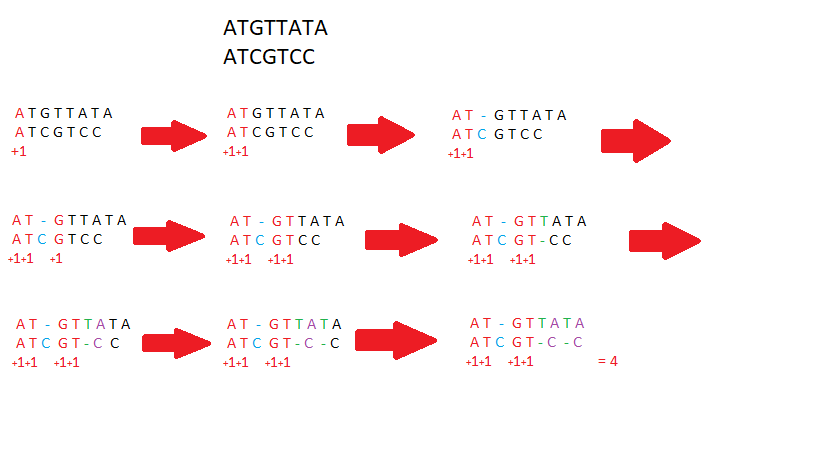
\includegraphics[width=0.7\textwidth]{poglavlja/5/slike/igraPoravnavanja.png}
\caption{Igra poravnanja}
\end{figure} 

\textbf{Poravnanje} dve sekvence predstavlja matricu koja ima dva reda:

\begin{enumerate}
    \item red: simboli prve sekvence (redom) eventualno sa ubačenim “-” 
    \item red: simboli druge sekvence (redom) eventualno sa ubačenim “-” 
\end{enumerate}
\begin{figure}[h!]
\centering
\includegraphics[width=0.4\textwidth]{poglavlja/5/slike/poravnanje.png}
\caption{Poravnanje}
\label{slika:poravnavanje}
\end{figure} 

\subsection{Najduža zajednička podsekvenca}

Poklapanja (matches) u poravnanju dve sekvence ( u primeru \ref{slika:poravnavanje} to je ATGT) formiraju njihovu zajedničku podsekvencu.
\begin{problem}[Problem najduže zajedničke podniske]
	Naći najdužu zajedničku podsekvencu dve niske. \\
	Ulaz: Dve niske. \\
	Izlaz: Najduža zajednička podsekvenca ovih niski
\end{problem}
%%%%%%%%%%%%%%%%%%%%%%%%%%%%%%%%%%%%%%%%%%%%

\section{Problem turiste na Menhetnu}

\noindent Pre svega postavimo problem:\\

\begin{problem}[Problem turiste na Menhetnu]
	Naći najdužu putanju u pravougaonoj mreži gradskih ulica. \\
	Ulaz: Usmeren težinski mrežni graf. \\
	Izlaz: Najduža putanja od početnog (source) do krajnjeg čvora (sink) u mrežnom grafu. 
\end{problem}

\begin{figure}[h!]
\centering
\includegraphics[width=0.7\textwidth]{poglavlja/5/slike/menhetn2.png}
\caption{Problem turiste na Menhetnu}
\label{slika:menhetn}
\end{figure} 

Na slici \ref{slika:menhetn} grafički je prikazan problem turiste na Menhetnu. Cilj je stići od plavog do crvenog kruga i pri tom sakupiti što više poena. Dozvoljeno kretanje je dole i desno. Možemo koristiti pohlepni algoritam i tako doći do cilja, ali da li smo tako sakupili najviše poena?

\noindent Dodatna izmena grafa bi bila da imamo i dijagnalne grane (\ref{slika:menhetn3}).

\begin{figure}[h!]
\centering
\includegraphics[width=0.7\textwidth]{poglavlja/5/slike/menhetn3.png}
\caption{Nepravilna mreža}
\label{slika:menhetn3}
\end{figure}

\noindent Time dolazimo do sledećeg problema:

\begin{problem}[Problem najduže putanje u usmerenom grafu]
	Naći najdužu putanju između dva   čvora u težinskom usmerenom grafu. \\
	Ulaz: Usmereni težinski graf sa označenim
čvorovima source i sink. \\
	Izlaz: Najduža putanja od čvora source do čvora
sink u usmerenom težinskom grafu. 
\end{problem}

Ako se prisetimo igre poravnanja, videćemo da postoji veza između ova dva problema (igre).

\begin{figure}[h!]
\centering
\includegraphics[width=0.7\textwidth]{poglavlja/5/slike/menhetn4.png}
\caption{Poravnanje $\rightarrow$ Putanja}
\label{slika:menhetn4}
\end{figure}

Pitamo se kako izgraditi graf za igru poravnanja i za problem najduže podsekvence. To ćemo uraditi na sledeći način:

\begin{itemize}
    \item Vrste označimo aminokiselinama iz prve niske
    \item Kolone označimo aminokiselinama iz druge niske
    \item U svaku presečnu tačku postavimo jedan čvor
    \item Gde god je moguće, postaviti vertikalne (insercija), horizontalne (delecija) i dijagonalne grane (match ili mismatch)
    \item Dijagonalne grane otežati koeficijentom 1, ostale koeficijentom 0
    \item Problem najduže zajedničke podsekvence se svodi na problem nalaženja najduže putanje između dva data čvora u usmerenom grafu
\end{itemize}

Kada nađemo poravnanje najvišeg skora našli smo i najdužu putanju u mrežnom grafu.

\begin{figure}[h!]
\centering
\includegraphics[width=0.7\textwidth]{poglavlja/5/slike/poravnanje1.png}
\caption{Poravnanje $\rightarrow$ Putanja}
\label{slika:poravnanje2}
\end{figure}

Dijagonalne crvene grane odgovaraju poklapanju simbola i imaju skor 1 (\ref{slika:poravnanje2})

%%%%%%%%%%%%%%%%%%%%%%%%%%%%%%%%%%%%%jasmina%%%%%%%%%%%%%%%%%%%%%%%%%%%%%%%%%%%%%%%%%%%%%%%%%%%%%%%%%%%%%%%%%%%%%%%%%%%%%%%%%%%%%%%%%%%%%%%%%%%%%%%%
\section{Problem kusura}

\noindent Upoznajmo se sa sledećim problemom:\\

\begin{problem}[Problem vraćanja kusura]
	Naći minimalan broj novčića neophodnih za vraćanje kusura. \\
	Ulaz: Ceo broj money i niz pozitivnih celih brojeva $(coin_1, coin_2, ..., coin_d)$. \\
	Izlaz: Minimalan broj novčića $(coin_1, coin_2, ..., coin_d)$ u apoenima koji rasitnjava sumu money. \\
\end{problem}

\subsection{Pohlepni algoritam}

Najzastupljeniji način vraćanja kusura širom sveta podrazumeva iterativno traženje sledećeg najvećeg novčića.\\
To bi značilo da bismo za kusur od 42 dinara dobili sledeće novčiće: 20 + 10 + 10 + 2. \\
Ovakav način vraćanja kusura opisuje takozvani pohlepni algoritam. \\

\begin{lstlisting}
GreedyChange(money)
begin
    change %$\leftarrow$% empty collection of coins
	while money > 0
		coin %$\leftarrow$% largest denomination that does not exceed money
		add coin to change
		money %$\leftarrow$% money - coin
	return change
end
\end{lstlisting}

Međutim, ako malo bolje razmislimo ovo rešenje zapravo nije najbolje.\\
Kusur bismo mogli vratiti i sa manje novčića na sledeći način: 42 = 20 + 20 + 2 \\

\textit{Zaključak}: \textbf{GreedyChange ne daje optimalno rešenje!}

\subsection{Rekurzivni algoritam}

Pokušajmo sada da problem rešimo na drugačiji način koristeći rekurziju. \\
Za zadate apoene 6, 5, 1, koji je najmanji broj novčića neophodnih za vraćanje kusura od 9 centi? \\

\begin{figure}[h!]
\centering
\includegraphics[width=0.7\textwidth]{poglavlja/5/slike/rekurzija1.JPG}
\caption{Vracanje kusura - rekurzija}
\label{slika:rekurzija}
\end{figure}

Problem resavamo tako sto prvo od 9 oduzmemo 6 i dobijemo 3 kao ostatak kusura. Dakle, 9 se može vratiti od jednog novčića od 6 apoena i jos plus broj novčiča koji je potreban za preostali deo kusura od 3 centa. \\
U istoj iteraciji analogno računamo za preostale apoene.\\

Na slici \ref{slika:rekurzija} crvenim znakom pitanja označeno je traženo rešenje koje dobijemo rešavanjem manjih problema za kusure 3, 4 i 8. \\ 

MinNumCoins(9) = $\min$ 
$\begin{cases}$
$MinNumCoins(9-6) + 1 = MinNumCoins(3) + 1\\$
$MinNumCoins(9-5) + 1 = MinNumCoins(4) + 1\\$
$MinNumCoins(9-1) + 1 = MinNumCoins(8) + 1\\$
$\end{cases}$

Na osnovu prethodnog, moguće je izvesti opštu formulu:

MinNumCoins(money) = $\min$ 
$\begin{cases}$
$MinNumCoins(money-coin_{1}) + 1 \\$
$\dots \\$
$MinNumCoins(money-coin_{d}) + 1 \\$
$\end{cases}$
\\
Hajde sada da vidimo kako bismo to isprogramirali:
\\
\begin{lstlisting}
RecursiveChange(money, coins)
begin
    if money = 0
        return 0
    MinNumCoins %$\leftarrow$% infinity 
    for i %$\leftarrow$% 1 to |coins|
        if money %$\geq coin_{i}$%
            NumCoins %$\leftarrow$% RecursiveChange(money - %$coin_{i}$%, coins)
            if numCoins + 1 < MinNumCoins
                MinNumCoins %$\leftarrow$% numCoins + 1
	return MinNumCoins
end
\end{lstlisting}

Reklo bi se da smo sada dobili odgovarajuci algoritam za naš problem, hajde to da proverimo. \\
Postavlja se pitanje, koliko je brz RecursiveChange? \\

Pokušajmo na konkretnom primeru da dođemo do rešenja. Neka naš problem sada bude vraćanje kusura od 76 centi. Pomoću rekurzivnog stabla demonstrirajmo ponašanje našeg algoritma: \\

\begin{figure}[h!]
\centering
\includegraphics[width=0.7\textwidth]{poglavlja/5/slike/rekurzivnoStablo.JPG}
\caption{Vracanje kusura - ponašanje rekurzivnog algoritma}
\label{slika:rekurzija2}
\end{figure}

Ono što se odmah može primetiti jeste višestruko pozivanje algoritma za vrednost od 69 centi, čak 6 puta! \\
Daljim procenama možemo doći do zaključka da se optimalna kombinacija novčića za 30 centi izračunava milijardama puta! \\

Sada je očigledno da nam rekurzija ne rešava problem na najbolji mogući način. \\

\subsection{Vraćanje kusura dinamičkim programiranjem}

Cilj nam je da izbegnemo višestruka izračunavanja  vraćanja kusura za istu vrednost, tako da bi ideja bila da imamo objekat koji će pamtiti sva računanja i iz koga ćemo čitati već izračunate vrednosti. \\
Dakle, umesto vremenski zahtevnih poziva \\
\begin{center}
RecursiveChange(money - $coin_{i}$, coins)
\end{center}
jednostavno bismo potražili vrednosti iz unapred izračunate tabele \\
\begin{center}
MinNumCoins(money - $coin_{i}$).
\end{center}


\begin{lstlisting}
DPChange(money, coins)
begin
    MinNumCoins(0) %$\leftarrow$% 0 
    for m %$\leftarrow$% 1 to money
        MinNumCoins(m) %$\leftarrow$% infinity
        for i %$\leftarrow$% 1 to |coins|
            if m %$\geq coin_{i}$%
                if MinNumCoins(m - %$coin_{i}$%) + 1 < MinNumCoins(m)
                    MinNumCoins(m) %$\leftarrow$% MinNumCoins(m - %$coin_{i}$%) + 1
	return MinNumCoins(money)
end
\end{lstlisting}


\section{Dinamičko programiranje i putokazi za povratak}

Posmatramo jednostavniji, Menhetn graf:
Pretpostavimo da do čvora sink možemo doći samo na dva načina: kretanjem južno $\downarrow$ ili kretanjem istočno $\rightarrow$

\begin{figure}[h!]
\centering
\includegraphics[width=0.7\textwidth]{poglavlja/5/slike/putokazi.png}
\caption{Južno ili istočno?}
\label{slika:putokazi}
\end{figure}

\noindent Prvo probamo da rešimo problem rekurzivno:

\begin{lstlisting}
SouthOrEast(n, m)
if n=0 and m=0
    return 0
x %$\leftarrow$% -infinity, y %$\leftarrow$% -infinity
if n > 0
x %$\leftarrow$% SouthOrEast(n-1,m)+weight of edge "%$\downarrow$%" into (n, m)
if m > 0
y %$\leftarrow$% SouthOrEast(n,m-1)+ weight of edge "%$\rightarrow$%" into (n,m)
return max{x, y}
\end{lstlisting}

\noindent Ovaj algoritam se poziva za svaki čvor u grafu veličine $m\times n$, a pri tom se dešava da za jedan isti čvor računamo više puta. Zbog toga je ovaj pristup previše spor, pa prelazimo na dinamičko programiranje.
Krenućemo  od početnog čvora. Zatim, u čvor (i, j) upisujemo dužinu maksimalne putanje od (0,0) do (i,j). Prvo izračunamo za čvorove na obodu grafa a zatim, kolonu po kolonu, za preostale čvorove.

\begin{figure}[h!]
\centering
\includegraphics[width=0.5\textwidth]{poglavlja/5/slike/putokazi1.png}
\caption{Južno ili istočno?}
\label{slika:putokazi1}
\end{figure}

\begin{figure}[h!]
\centering
\includegraphics[width=0.5\textwidth]{poglavlja/5/slike/putokazi2.png}
\caption{Južno ili istočno?}
\label{slika:putokazi2}
\end{figure}

\begin{figure}[h!]
\centering
\includegraphics[width=0.5\textwidth]{poglavlja/5/slike/putokazi3.png}
\caption{Južno ili istočno?}
\label{slika:putokazi3}
\end{figure}

Na slici \ref{slika:putokazi3} prikazane su podebljane grane koje predstavljaju putokaze za povratak od čvora sink do čvora source.

\subsection{Rekurentna relacija dinamičkog programiranja kod Menhetn grafa}

$s_i,_j$: the length of a longest path from (0,0) to (i,j)

$s_i,_j$ = $\max$ $\begin{cases}$
$s_{i-1},_j + weight of edge "\downarrow"into (i,j)\\$
$s_i,_{j-1} + weight of edge "\rightarrow"into (i,j)$
$\end{cases}$

\begin{lstlisting}
ManhattanTourist(n, m, Down, Right)
%$s_0,_0$% %$\leftarrow$% 0
for i %$\leftarrow$% 1 to n
    %$s_i,_0$% %$\leftarrow$% %$s_{i-1},_0$% + %$down_i,_0$%
for j %$\leftarrow$% 1 to m
    %$s_0,_j$% %$\leftarrow$% %$s_0,_{j-1}$% + %$right_0,_j$% 
for i %$\leftarrow$% 1 to n
    for j %$\leftarrow$% 1 to m
        %$s_i,_j$% %$\leftarrow$% %$\max$% { %$s_{i-1},_j$% + %$down_i,_j$%, %$s_i,_{j-1}$% + %$right_i,_j$% }
return %$s_n,_m$%
\end{lstlisting}



%%%%%%%%%%%%%%%%%%%%%%%%%%%%%%%%%%%%%%%%%%%%%%%%%%%%%%%%%%%%%%%%%%%%%%%%%

\section{Od Menhetna do grafa poravnanja }

\subsection{Rekurentna relacija dinamičkog programiranja kod grafa poravnanja}


Najduži put (slika \ref{slika:povratak}) od (0,0) do (i,j) se računa:


$s_i,_j$ = $\max$ $\begin{cases}$
$s_{i-1},_j$ + 
$\textcolor{green}{weight\ of\ edge\ "\downarrow"\ into\ (i,j)}\\$
$s_i,_{j-1}$ + 
$\textcolor{blue}{weight\ of\ edge\ "\rightarrow"\ into\ (i,j)}\\$
$s_{i-1},_{j-1}$ + 
$\textcolor{red}{weight\ of\ edge\ "\searrow"\ into\ (i,j)}$
$\end{cases}$

Što dalje daje :

$s_i,_j$ = $\max$ $\begin{cases}$
$\textcolor{green}{s_{i-1},_j + 0}\\$
$\textcolor{blue}{s_i,_{j-1} + 0}\\$
$\textcolor{red}{s_{i-1},_{j-1} + 1, v_i = w_j}\\$
$\textcolor{red}{s_{i-1},_{j-1} + 0, v_i \neq w_j}$
$\end{cases}$



\begin{figure}[h!]
\centering
\includegraphics[width=0.5\textwidth]{poglavlja/5/slike/graf1.png}
\caption{ Crvene grane težina 1, ostale grane težina 0, $v_i$ i $w_j$ oznake vrste i kolone}
\label{slika:povratak}
\end{figure}


U slici \ref{slika:backtrack} se vide boldovane grane koje su nastale primenom pravila rekurentne relacije. One predstavljaju putokaze za povratak (backtrack) kod grafa za najdužu zajedničku podsekvencu. 

\begin{figure}[h!]
\centering
\includegraphics[width=0.5\textwidth]{poglavlja/5/slike/backtrack.png}
\caption{Putokazi za povratak (backtrack)}
\label{slika:backtrack}
\end{figure}

\subsection{Računanje putokaza za povratak }

$s_i,_j$ $\leftarrow$ $\max$ $\begin{cases}$
$\textcolor{green}{s_{i-1},_j + 0}\\$
$\textcolor{blue}{s_i,_{j-1} + 0}\\$
$\textcolor{red}{s_{i-1},_{j-1} + 1, v_i = w_j}\\$
$\textcolor{red}{s_{i-1},_{j-1} + 0, v_i \neq w_j}$
$\end{cases}$


$backtrack_i,_j$  $\leftarrow$  $\max$ $\begin{cases}$
$\textcolor{blue}{ "\rightarrow", s_i,_j = s_{i},_{j-1}}\\$
$\textcolor{green}{ "\downarrow", s_i,_j = s_{i-1},_j}\\$
$\textcolor{red}{"\searrow", otherwise}$
$\end{cases}$


Podsetimo se sada kako bismo rekontruisali putanju preko putokaza kod Menhetn grafa? Krenuli bismo od krajnjeg čvora (sink) i pratili putokaze u obrnutom smeru do početnog čvora (source) \ref{slika:rek3}.\\
\begin{figure}[h!]
\centering
\includegraphics[width=0.7\textwidth]{poglavlja/5/slike/rek3.png}
\caption{Rekonstrukcija putanje preko putokaza kod Menhetn grafa}
\label{slika:rek3}
\end{figure}

\begin{figure}[h!]
\centering
\includegraphics[width=0.5\textwidth]{poglavlja/5/slike/backtrackNajduzaZajPS.png}
\caption{Backtracking}
\label{slika:backNZPS}
\end{figure}
Sada na slici \ref{slika:backNZPS} možemo videti povratak (backtracking) kod grafa za najdužu zajedničku podsekvencu.

\subsection{Određivanje najduže zajedničke podsekvence (LCS – longest common subsequence) korišćenjem putokaza za povratak}

\begin{lstlisting}
OutputLCS (backtrack, v, i, j)
if i = 0 or j = 0
    return
if %$backtrack_i,_j$% = "%$\rightarrow$%"
    OutputLCS (backtrack, v, i, j-1)
else if %$backtrack_i,_j$% = "%$\downarrow$%"
    OutputLCS (backtrack, v, i-1, j)
else
    OutputLCS (backtrack, v, i-1, j-1)
    output  %$v_i$%
\end{lstlisting}

Do sada smo pretpostavljali da graf u kom tražimo
najdužu putanju ima samo tri vrste grana. Da li se OutputLCS može generalizovati tako da važi i za grafove koji nemaju tako specifičnu
topologiju?\\
Kako se rekurentna relacija dinamičkog programiranja menja za ovakav graf? \ref{slika:rekRel}
\begin{figure}[h]
\centering
\includegraphics[width=\textwidth]{poglavlja/5/slike/rekurentaRelDinProg.png}
\caption{}
\label{slika:rekRel}
\end{figure}
\\

\textit{$s_a$ = $max_{all\ predecessors\ b\ of\ node\ a}$\{$s_b$+ weight of edge from b to a\}}
\\

Računanje skora za SVE prethodnike \ref{slika:racunanje}.

\begin{figure}[h]
\centering
\includegraphics[width=0.7\textwidth]{poglavlja/5/slike/racunanje.png}
\caption{Začarani krug}
\label{slika:racunanje}
\end{figure}

\begin{itemize}
    \item Kod ovakve rekurentne relacije, važno je da pri računanju $s_a$ imamo izračunate $s_b$ za sve čvorove prethodnike b (čvorovi za koje
postoji grana do čvora a) Da li je to moguće u bilo kom usmerenom
težinskom grafu? Odgovor je \textbf{nije}. Da bismo kod svakog čvora mogli da mogli da izračunamo skor za sve njegove prethodnike, usmereni težinski graf mora biti acikličan. DAG (Directed Acyclic Graph) 
    \item Ako je dat usmereni aciklični graf, da li njegove čvorove možemo poređati u niz tako da njihov redosled u nizu osigurava uslov da pri računanju $s_a$ imamo izračunate $s_b$ za sve čvorove prethodnike b (čvorovi za koje postoji grana do čvora a)? Odgovor je \textbf{da}, moguće je poređati sve čvorove grafa u niz i taj niz topološki sortirati
\end{itemize}




\subsection{Topološko sortiranje}

\begin{itemize}
    \item \textbf{Topološko sortiranje} : Sortiranje čvorova DAG-a u nizu tako da sve grane u takvom nizu idu s leva na desno.
    \item \textbf{ Teorema}: Svaki DAG se može topološki sortirati.
    \item Topološko sortiranje svakog DAG-a se obavlja za O(\#edges) koraka.
\end{itemize}

\textbf{Algoritam za nalaženje najduže putanje u DAG-u>} :

\begin{lstlisting}
LongestPath(Graph, source, sink)
for each node a in Graph
     %$s_a$% %$\leftarrow$% -%$\infty$%
%$s_{source}$% %$\leftarrow$%  0
topologically order Graph
for each node a (from source to sink in topological order)
%$s_a$%  %$\leftarrow$% %$max_{all\ predecessors\ b\ of\ node\ a}$% {%$s_b$% + weight of edge from b to a}
return %$s_{sink}$%
\end{lstlisting}


\begin{itemize}
    \item Pošto svaka grana učestvuje tačno jednom, složenost je O(\#edges)
    \item LongestPath vraća dužinu najdužeg zajedničkog podniza ali ne rekonstruiše putanju
\end{itemize}

%%%%%%%%%%%%%%%%%%%%%%%jasminaaaaaa%%%%%%%%%%%%%%%%%%%%%%%%%%%%%%%%%%%%%%%%%
\section{Od globalnog do lokalnog poravnanja}

\noindent Uvedimo sledeće:
\begin{itemize}
    \item Skor poravnanja do sada - $\#\textcolor{red}{matches}$ \\
    \item Skor sa mismatch i indel kaznama - $\#\textcolor{red}{matches} - \textcolor{purple}{\mu} * \#\textcolor{purple}{mismatches} - \sigma * \#\textcolor{blue}{in}\textcolor{green}{dels}$ \\
\end{itemize}

Primer na slici \ref{slika:matriceSkora}. \\

\begin{figure}[H]
\centering
\includegraphics[width=\textwidth]{poglavlja/5/slike/matriceSkora.JPG}
\caption{}
\label{slika:matriceSkora}
\end{figure}

Navedimo rekurentnu relaciju dinamičkog programiranja kod grafa poravnanja. Počinjemo od:

$s_i,_j$ = $\max$ $\begin{cases}$
$s_{i-1},_j$ + 
$\textcolor{green}{weight\ of\ edge\ "\downarrow"\ into\ (i,j)}\\$
$s_i,_{j-1}$ + 
$\textcolor{blue}{weight\ of\ edge\ "\rightarrow"\ into\ (i,j)}\\$
$s_{i-1},_{j-1}$ + 
$\textcolor{red}{weight\ of\ edge\ "\searrow"\ into\ (i,j)}$
$\end{cases}$

Odnosno, \\
\\
$s_i,_j$ = $\max$ $\begin{cases}$
$\textcolor{green}{s_{i-1},_j - \sigma}\\$
$\textcolor{blue}{s_i,_{j-1} - \sigma}\\$
$\textcolor{red}{s_{i-1},_{j-1} + 1, v_i = w_j}\\$
$\textcolor{purple}{s_{i-1},_{j-1} - \mu, v_i \neq w_j}\\$
$\end{cases}$
\\
A uz pomoc funkcije $score()$ može se zapisati i kao: \\
\\

\begin{figure}[!htb]
     \begin{minipage}{0.49\textwidth}
        $s_i,_j$ = $\max$ $\begin{cases}$
        $\textcolor{green}{s_{i-1},_j + score(v_i, -)}\\$
        $\textcolor{blue}{s_i,_{j-1} + score(-, w_j)}\\$
        $\textcolor{red}{s_{i-1},_{j-1} score(v_i, w_j)}\\$
        $\end{cases}$
     \end{minipage}
     \hfill
     \begin{minipage}{0.49\textwidth}
       \includegraphics[width=\linewidth]{poglavlja/5/slike/rekurentna.JPG}
       \caption{}\label{}
     \end{minipage}
   \end{figure}
   
\subsection{Globalno poravnanje}

\begin{problem}[Problem globalnog poravnanja]
	Naći poravnanje sa najvišim skorom između dve niske za datu matricu skora. \\
	Ulaz: Niske v i w, kao i matrica skora score \\
	Izlaz: Poravnanje niski v i w čiji je skor poravnanja (prema matrici skora) maksimalan od svih mogućih poravnanja v i w. 
\end{problem}

\noindent Šta bi bili homeobox geni? \\
\begin{itemize}
    \item Dva gena u različitim vrstama mogu biti slična u kratkim, konzervativnim regionima, a različita u ostalim delovima.
    \item Homeobox geni sadrže kratak region homeodomen koji je čvrsto konzerviran među različitim vrstama.
    \item Globalno poravnanje može da propusti nalaženje homeodomena jer pokušava da poravna sekvence u celosti.
\end{itemize}

\noindent Uporedimo sledeća dva poravnanja: \\
\begin{figure}[!htb]
 \begin{minipage}{0.49\textwidth}
    \includegraphics[width=\linewidth]{poglavlja/5/slike/globalno.JPG}
   \caption{}\label{}
   score = 22(matches) - 2(indent) = 2
 \end{minipage}
 \hfill
 \begin{minipage}{0.49\textwidth}
   \includegraphics[width=\linewidth]{poglavlja/5/slike/lokalno.JPG}
   \caption{}\label{}
   score = 17 (matches) - 30(indent) = -13
 \end{minipage}
\end{figure}
   
\begin{figure}[!htb]
 \begin{minipage}{0.49\textwidth}
    \includegraphics[width=\linewidth]{poglavlja/5/slike/grafik_poravnanje1.JPG}
   \caption{}\label{}
 \end{minipage}
 \hfill
 \begin{minipage}{0.49\textwidth}
   \includegraphics[width=\linewidth]{poglavlja/5/slike/grafik_poravnanje2.JPG}
   \caption{}\label{}
 \end{minipage}
\end{figure}

\noindent Ako se zapitamo koje od njih je bolje, iz priloženog zaključujemo da je to lokalno poravnanje.\\

\subsection{Lokalno poravnanje}

Lokalno poravnanje računamo kao globalno poravnanje u pravougaoniku, pogledajmo sliku \ref{slika:pravougaonici}. \\

\begin{figure}[H]
 \begin{minipage}{0.49\textwidth}
    \includegraphics[width=\linewidth]{poglavlja/5/slike/lokalno_poravnanje_pravougaonici1.JPG}
   \caption{}\label{}
 \end{minipage}
 \hfill
 \begin{minipage}{0.49\textwidth}
   \includegraphics[width=\linewidth]{poglavlja/5/slike/lokalno_poravnanje_pravougaonici2.JPG}
   \caption{}\label{slika:pravougaonici}
 \end{minipage}
\end{figure}

\noindent Da bismo dobili lokalno poravnanje potrebno je da izračunamo globalno poravnanje u okviru svakog pravougaonika.\\
Algoritam globalnog poravnanja ponovićemo između svaka dva čvora, ne samo između početnog (source) i krajnjeg (sink). \\
Stoga, broj ponavljanja algoritma će biti $\#nodes ^ 2$ puta. \\

\begin{problem}[Problem lokalnog poravnanja]
	Naći lokalno poravnanje najvećeg skora između dve niske. \\
	Ulaz: Niske v i w, kao i matrica skora score \\
	Izlaz: Podniske niski v i w čije je globalno poravnanje (prema matrici skora) maksimalno među svim globalnim poravnanjima svih podniski niski v i w. 
\end{problem}

\noindent Zamislimo da postoji taksi koji bi nas besplatno vozio do tačke početka lokalnog poravnanja, i od tačke završetka lokalnog poravnanja pa do kraja. Na taj način ne bismo skupili negativne poene, već samo pozitivne. Ovakva vožnja nam daje samo skor lokalnog poravnanja kao što smo i želeli. \ref{slika:taksiFree}\\
 
 \begin{figure}[H]
\centering
\includegraphics[width=0.7\textwidth]{poglavlja/5/slike/free_taxi.JPG}
\caption{Besplatne taksi vožnje}
\label{slika:taksiFree}
\end{figure} 

Konstruišimo Menhetn graf za problem lokalnog poravnanja: \\

\begin{figure}[H]
     \begin{minipage}{0.59\textwidth}
        Kako bi izgledao Menhetn graf za nas problem? \\
        Dodamo grane težine 0 od (0,0) do svakog čvora, i od svakog čvora do (n,m). \\
        Ukupan broj dodatih grana je $O(|v|+|w|)$, pa algoritam ostaje brz. \\
     \end{minipage}
     \hfill
     \begin{minipage}{0.39\textwidth}
       \includegraphics[width=\linewidth]{poglavlja/5/slike/free_taxi_graf.JPG}
       \caption{Menhetn graf za lokalno poravnanje}\label{}
    \end{minipage}
\end{figure}

Problem rešavamo dinamičkim programiranjem: \\

\begin{figure}[H]
     \begin{minipage}{0.59\textwidth}
        $s_i,_j$ = $\max$ $\begin{cases}$
        $s_{i-1},_j$ + 
        $\textcolor{green}{weight\ of\ edge\ "\downarrow"\ into\ (i,j)}\\$
        $s_i,_{j-1}$ + 
        $\textcolor{blue}{weight\ of\ edge\ "\rightarrow"\ into\ (i,j)}\\$
        $s_{i-1},_{j-1}$ + 
        $\textcolor{red}{weight\ of\ edge\ "\searrow"\ into\ (i,j)}$
        $\end{cases}$
     \end{minipage}
     \hfill
     \begin{minipage}{0.39\textwidth}
       \includegraphics[width=\linewidth]{poglavlja/5/slike/lokalno_poravnanje_0.JPG}
       \caption{weight of (0,0) into (i,j) = 0}\label{}
    \end{minipage}
\end{figure}


%%%%%%%%%%%%%%%%%%%%%%%%%%%%%%%%%%%%%%%%%%%%%%%%%%%%%%%%%%%%%%%%%%%%
\section{Kažnjavanje insercija i delecija u poravnanju sekvenci}

\subsection{Kažnjavanje praznina}

\begin{itemize}
    \item U globalnom poravnanju je fiksna kazna $\sigma$ bila dodeljena svakom indelu
    \item Međutim, ova fiksna kazna može biti preoštra
kod lokalnog poravnanja kada možemo imati 100 uzastopnih indela.
    \item Niz od k uzastopnih indela često predstavlja jedan isti evolucioni događaj, ne k različitih, slika \ref{slika:kaznjavanje}
\end{itemize}

\begin{figure}[h]
\centering
\includegraphics[width=0.5\textwidth]{poglavlja/5/slike/kaznjavanjePraznina.png}
\caption{}
\label{slika:kaznjavanje}
\end{figure}

\subsection{Adekvatnije kazne za praznine}

\textbf{Afina kazna za praznine} za prazninu dužine k:  \textbf{$\sigma+\epsilon*(k-1)$}
\begin{itemize}
    \item $\sigma$ kazna za \textbf{otvaranje} praznine
    \item $\epsilon$ kazna za \textbf{proširenje} praznine
    \item $ \sigma > \epsilon$ , jer otvaranje praznine treba kazniti više nego njeno proširenje
\end{itemize}



U slici \ref{slika:modelovanje} prikayano je modelovanje afinih kazni za praznine pomoću dugih grana.

\begin{figure}[h!]
\centering
\includegraphics[width=0.7\textwidth]{poglavlja/5/slike/modelovanjePomocuDugihGrana.png}
\caption{Modelovanje afinih kazni za praznine pomoću dugih grana}
\label{slika:modelovanje}
\end{figure}

\subsection{Izgradnja Menhetn grafa sa afinim kaznama za praznine}

\begin{figure}[h!]
\centering
\includegraphics[width=0.5\textwidth]{poglavlja/5/slike/MenhettnAifnePraznine.png}
\caption{Dodali smo $O(n^3)$ grana}
\label{slika:afiniMenhetn}
\end{figure}


\begin{itemize}
    \item Vremenska složenost je direktno proporcionalna broju grana, zbog čega želimo da smanjimo broj grana u grafu (trenutno je
$O(n^3)$ \ref{slika:afiniMenhetn})
\item Jedan način za smanjivanje broja grana je povećanje broja čvorova u grafu
\item Zato delimo Menhetn graf na tri nivoa \ref{slika:triNivoa}
\end{itemize}


\begin{figure}[h!]
\centering
\includegraphics[width=\textwidth]{poglavlja/5/slike/triNivoa.png}
\caption{Podela Menhetna grafa na 3 nivoa}
\label{slika:triNivoa}
\end{figure}

Ako imamo putanju poput one na slici \ref{slika:kakoSimulirati}, kako da je predstavimo pomoću Menhetn grafa na 3 nivoa? Rešenje je prikazano na slici \ref{slika:simulacija}


\begin{figure}[h!]
\centering
\includegraphics[width=0.5\textwidth]{poglavlja/5/slike/kakoSimulirari.png}
\caption{Kako predstaviti pomoću Menhetn grafa na 3 nivoa?}
\label{slika:kakoSimulirati}
\end{figure}


\begin{figure}[h!]
\centering
\includegraphics[width=0.7\textwidth]{poglavlja/5/slike/simulacija.png}
\caption{Simulacija Menhetn grafa na 3 nivoa}
\label{slika:simulacija}
\end{figure}

%%%%%%%%%%%%%%%%%%%%%%%%%%%%%%%%%jasminaaaa%%%%%%%%%%%%%%%%%%%%%%%%%%%%%%%%%%%

\section{Prostorno efikasno poravnanje sekvenci}

Zapitajmo se sledeće: \\
Da li možemo poravnati NPR sintetaze iz dve različite bakterije? \\
\\

Uzmimo u obzir sledeće činjenice:
\begin{itemize}
    \item NPR sintetaze su obično veoma dugi proteini, približno 20 000 aminokiselina
    \item Vremenska složenost poravnanja je probližno jednaka broju ivica (\#edges), odnosno kvadratna
    \item Prostorna složenost poravnanja je probližno jednaka broju čvorova (\#nodes), odnosno kvadratna
    \item \textbf{Memorija je često usko grlo pri poređenju dugih sekvenci}
\end{itemize}

Iz prethodnog zaključujemo da nam prostorna složensot pravi problem i da bi za prosečan racunar ovo bilo nemoguće da izračuna. 
Stoga, potreban nam je drugi pristup koji će nam rešiti problem. Potreban nam je algoritam koji zahteva linearnu prostornu složenost i udvostručenu vremensku složenost. U te svrhe najčešće se koristi algoritam koji radi po principu podeli-pa-vladaj. \\

Uvedimo nove pojmove:
\begin{itemize}
    \item Srednja kolona poravnanja (middle) $= \#columns/2$, slika \ref{slika:srednjaKolona}
    \item Srednji čvor poravnanja - čvor u preseku putanje optimalnog poravnanja i srednje kolone, slika \ref{slika:srednjiCvor}
\end{itemize}


\begin{figure}[h!]
\centering
\includegraphics[width=0.5\textwidth]{poglavlja/5/slike/srednjaKolona.JPG}
\caption{Srednja kolona poravnanja}
\label{slika:srednjaKolona}
\end{figure}

\begin{figure}[h!]
\centering
\includegraphics[width=0.5\textwidth]{poglavlja/5/slike/srednjiCvor.JPG}
\caption{Srednji čvor poravnanja}
\label{slika:srednjiCvor}
\end{figure}

Koristeći navedene pojmove, demonstrirajmo algoritam \textbf{Podeli-pa-vladaj} za poravnanje sekvenci, slika \ref{slika:podeliPaVladaj}: \\

\begin{lstlisting}
AlignmentPath(source, sink)
    find middleNode
    AlignmentPath(source, middleNode)
    AlignmentPath(middle, sink)
\end{lstlisting}

\begin{figure}[h!]
\centering
\includegraphics[width=0.5\textwidth]{poglavlja/5/slike/podeliPaVladaj.JPG}
\caption{Srednja kolona poravnanja}
\label{slika:podeliPaVladaj}
\end{figure}

\subsection{Prostorna složenost}
Za nalaženje najduže putanje u grafu poravnanja traži se čuvanje svih putokaza za - $O(nm)$ prostora. \\
Međutim, za nalaženje dužine najduže putanje u grafu poravnanja ne traži se čuvanje svih putokaza - $O(n)$ prostora, slika \ref{slika:prostornaSlozenost}

\begin{figure}[h!]
\centering
\includegraphics[width=0.5\textwidth]{poglavlja/5/slike/prostornaSlozenost2.JPG}
\caption{Recikliranje prostora za kolone u grafu poravnanja}
\label{slika:prostornaSlozenost}
\end{figure}

Dobijamo da je prostor potreban za algoritam $2*n \sim O(n)$, odnosno, linearan. \\ 

\subsection{Vremenska složenost}

Neka je \textbf{i-putanja} najduža putanja od svih putanja koja posećuje i-ti čvor u srednjoj koloni i neka je \textbf{$length(i)$} dužina i-putanje.\\

Na slici \ref{slika:iputanja} vidimo da je $length(0)=2$ i $length(4)=4$. \\


\begin{figure}[h!]
\centering
\includegraphics[width=0.5\textwidth]{poglavlja/5/slike/i_putanje.JPG}
\caption{Računanje length(i)}
\label{slika:iputanja}
\end{figure}


$length(i)$ možemo računati na sledeći način:
\begin{center}
$length(i) = fromSource(i) + toSink(i)$
\end{center}

\begin{figure}[h!]
\centering
\includegraphics[width=0.5\textwidth]{poglavlja/5/slike/i_putanje.JPG}
\caption{Računanje length(i)}
\label{slika:iputanja}
\end{figure}

Na slici \ref{slika:sourceSink} vidimo koliko je potrebno vremena za nalaženje srednjeg čvora - čak $O(nm)$ vremena za nalaženje samo jednog čvora! 
\begin{figure}[h!]
\centering
\includegraphics[width=0.5\textwidth]{poglavlja/5/slike/sourceSink.JPG}
\caption{Računanje vremena za nalaženje srednjeg čvora}
\label{slika:sourceSink}
\end{figure}

Svaki problem se može rešiti u vremenu proporcionalnom broju grana tj. površini koju zauzima. \\
Vreme potrebno za rešavanje naredna dva potproblema: $area/4 + area/4 = area/2$, znači  $O(nm + nm/2)$ vremena za nalaženje 3 čvora. \\
Dakle, vreme potrebno za nalaženje svih čvorova je: $area + area/2 + area/4 + area/8 + \dots < 2 * area$! Slika \ref{slika:vreme} vizuelno prikazuje vreme potrebno za nalaženje 7 tačaka. \\

\begin{figure}[h!]
\centering
\includegraphics[width=0.5\textwidth]{poglavlja/5/slike/vremenskaSlozenostPPV.JPG}
\caption{Računanje vremena za nalaženje 7 tačaka}
\label{slika:vreme}
\end{figure}

Pokazali smo da je vremenska složenost $2*n*m \sim O(n*m)$. \\
%%%%%%%%%%%%%%%%%%%%%%%%%%%%%%%%%%%%%%%%%%%%%%%%%%%%%%%%%%%%%%%%%%%%

\section{Višestruko poravnanje sekvenci}

\subsection{Od dvostrukog do višestrukog poravnanja}
\begin{itemize}
    \item Do sada su u poravnanju učestvovale samo dve sekvence.
    \item Slaba sličnost između dve sekvence postaje značajna ako je prisutna i u drugim sekvencama
    \item Višestruka poravnanja mogu otkriti suptilne sličnosti koje dvostruka poravnanja ignorišu
\end{itemize}

\subsection{Poravnanje tri A-domena}
Na slici \ref{slika:poravnavanjaTriA} je prikazano poravnanje tri A-domena
\begin{figure}[h!]
\centering
\includegraphics[width=\textwidth]{poglavlja/5/slike/poravnavanjaTriAdomena.png}
\caption{Poravnavanja 3 A-domena}
\label{slika:poravnavanjaTriA}
\end{figure}

\subsection{Generalizacija dvostrukog na višestroko poravnanje}
    
\begin{itemize}
    \item Poravnanje 2 sekvence je matrica od 2 reda
    \item Poravnanje 3 sekvence je matrica od 3 reda (slika  \ref{slika:poravnavanjeMatrica})
    \begin{figure}[h!]
    \centering
    \includegraphics[width=0.3\textwidth]{poglavlja/5/slike/poravnanjeMatrica.png}
    \caption{}
    \label{slika:poravnavanjeMatrica}
    \end{figure}
    \item Funkcija skora treba da dodeljuje visok skor poravnanjima sa konzerviranim kolonama
\end{itemize}



\subsection{Poravnanja = 3-D putanje}

Poravnanje sekvenci ATGC, AATC i ATGC \ref{slika:3d}

\begin{figure}[h]
\centering
\includegraphics[width=0.8\textwidth]{poglavlja/5/slike/3dPoravnanja.png}
\caption{Poravnanje sekvenci ATGC, AATC i ATGC}
\label{slika:3d}
\end{figure}

\subsection{2-D poravnanje u odnosu na 3-D poravnanje}
\begin{figure}[h]
\centering
\includegraphics[width=0.5\textwidth]{poglavlja/5/slike/2d3d.png}
\caption{}
\label{slika:2d3d}
\end{figure}
2-D poravnanje u odnosu na 3-D poravnanje prikazano na slici \ref{slika:2d3d}.

\subsection{Rekurentna relacija dinamičkog programiranja
za višestruko poravnanje}



$s_i,_j,_k$ = $\max$ $\begin{cases}$

$s_{i-1},_{j-1},_{k-1}$+ $\delta(v_i, w_j, u_k)\\$
$s_{i-1},_{j-1},_k$+ $\delta(v_i, w_j, -)\\$
$s_{i-1},_j,_{k-1}$+ $\delta(v_i, -, u_k)\\$
$s_i,_{j-1},_{k-1}$+ $\delta(-, w_j, u_k)\\$
$s_{i-1},_{j},_k$+ $\delta(v_i,-, -)\\$
$s_{i},_{j-1},_k$+ $\delta(-, w_j, -)\\$
$s_{i},_{j},_{k-1}$+ $\delta(-, -, u_k)\\$
$\end{cases}$

$\delta$(x, y, z) - element 3-D matrice skora

\subsection{Vremenska složenost dinamičkog algoritma
za višestruko poravnanje}

\begin{itemize}
    \item Kao kod dvostrukog poravnanja, vremenska složenost je proporcionalna broju grana O(\#edges)
    \item Za 3 sekvence n, vremenska složenost je proporcionalna 7$n^3$
    \item Za poravnanje k sekvenci, potrebno je izgraditi kdimenzionalni Menhetn graf sa: 
    \begin{itemize}
        \item  $n^k$ čvorova
        \item većina čvorova će imati $2^k – 1$ ulaznih grana
        \item Vremenska složenost: O($2^kn^k$)
    \end{itemize}
\end{itemize}


Višestruko poravnanje uključuje i dvostruko poravnanje, slika \ref{slika:visestrukoDvostruko}

\begin{figure}[h!]
\centering
\includegraphics[width=0.5\textwidth]{poglavlja/5/slike/visestrukoDvostruko.png}
\caption{}
\label{slika:visestrukoDvostruko}
\end{figure}

\subsection{Da li se višestruko poravnanje može izgraditi iz dvostrukog?}
Za dati skup proizvoljnih dvostrukih poravnanja, možemo li konstruisati višestruko poravnanje iz kog su izvedeni (slika \ref{slika:dvostruka})?

\begin{figure}[h!]
\centering
\includegraphics[width=0.7\textwidth]{poglavlja/5/slike/dvostruka.png}
\caption{}
\label{slika:dvostruka}
\end{figure}

\subsection{Profilna reprezentacija višestrukog poravnanja}

Na slici \ref{slika:profilVisetruko} prikazana profilna reprezentacija višestrukog poravnanja.
\begin{figure}[h!]
\centering
\includegraphics[width=0.6\textwidth]{poglavlja/5/slike/profilVisestruko.png}
\caption{}
\label{slika:profilVisetruko}
\end{figure}


\begin{itemize}
    \item Do sada smo poravnavali \textbf{sekvencu u odnosu na sekvencu.}
    \begin{itemize}
        \item Možemo li poravnati \textbf{sekvencu u odnosu na profil}?
        \item Možemo li poravnati \textbf{profil u odnosu na profil}?
    \end{itemize}
   
\end{itemize}


\subsection{Višestruko poravnanje: pohlepni pristup}

\begin{itemize}
    \item Izabrati najsličnije sekvence i kombinovati ih u profil
     \item Tako bismo smanjili broj sekvenci sa k na k-2 i jedan profil
    \item Iterirati
\end{itemize}

Primer pohlepnog pristupa:
\begin{itemize}
    \item Sekvence: GATTCA, GTCTGA, GATATT, GTCAGC
    \item 6 dvostrukih poravnanja (\textcolor{red}{match}+1, \textcolor{ForestGreen}{in}\textcolor{blue}{dels} i \textcolor{purple}{mismatches -1}) slika \ref{slika:sestDvostrukih}
    \begin{figure}[h!]
    \centering
    \includegraphics[width=0.5\textwidth]{poglavlja/5/slike/sestDvostrukih.png}
    \caption{}
    \label{slika:sestDvostrukih}
    \end{figure}
    \item Pošto su $s_2$ i $s_4$ najbliže, od njih pravimo profil
    
     \begin{figure}[h!]
    \centering
    \includegraphics[width=0.4\textwidth]{poglavlja/5/slike/profil.png}
    \caption{}
    \label{slika:profil}
    \end{figure}
    \item Novi skup od 3 sekvence za poravnanje:\\
            $s_1$ GATTCA\\
            $s_3$ GATATT\\
            $s_2,_4$ \textcolor{ForestGreen}{GTC}\textcolor{red}{t/a}\textcolor{ForestGreen}{G}\textcolor{red}{a/c}

\end{itemize}
%%% dodati tekst


%%%%%%%%%%%%%%%%%%%%%%%%%%%%%%%%%%%%%%%%%%%%%%%%%%%%%%%%%%%%%%%%%%%

\newpage
\section{Zadaci sa vežbi}
\setexamplecodestyle

U nastavku će biti predstavljeni zadaci sa vežbi na kursu rađeni u programskom jeziku Python.

\subsection{Manhattan Tourist}

\lstinputlisting[language=Python]{poglavlja/5/kodovi/ManhattanTourist.py}

\subsection{LCS Backtrack}

\lstinputlisting[language=Python]{poglavlja/5/kodovi/LCSBacktrack.py}

\subsection{Global Alignment}

\lstinputlisting[language=Python]{poglavlja/5/kodovi/GlobalAlignment.py}

\subsection{Local Alignment}

\lstinputlisting[language=Python]{poglavlja/5/kodovi/LocalAlignment.py}

\subsection{Edit Distance}

\lstinputlisting[language=Python]{poglavlja/5/kodovi/EditDistance.py}
\documentclass{article}

\usepackage[serbian, english]{babel}
\usepackage[utf8x]{inputenc}
\usepackage{fancyhdr}
\fancyhf{}
\fancyhead[L]{ščđćž}
\fancyhead[R]{\thepage}

\usepackage[T1]{fontenc}
%\setbookcodestyle
\usepackage{color}

\hyphenation{ci-klu-se}

\usepackage[labelformat=empty]{caption}

\usepackage{amsmath}
\usepackage{amssymb}
\usepackage{mathtools}
\usepackage{amsthm} 
\usepackage{gensymb}
\usepackage{listings}

\newcommand{\setexamplecodestyle}{
	\lstset{
		basicstyle=\ttfamily,
		columns=fullflexible,
		keepspaces=true,
		showstringspaces=false,
		escapechar=\%,
		tabsize=4,
		language=Python,
		breaklines=true,
		postbreak=\mbox{\textcolor{red}{$\hookrightarrow$}\space},
		frame=None,
	   	keywordstyle=\bfseries\color{green!40!black},
	   	commentstyle=\itshape\color{purple!40!black},
	   	identifierstyle=\color{blue},
	   	stringstyle=\color{orange}
	}
}


\usepackage{graphicx}
\usepackage[export]{adjustbox}
\graphicspath{ {images} }


%\addto\renewcommand{\figurename}{Slika}
\newtheorem{definicija}{Definicija}
\newtheorem{teorema}{Teorema}

\title{Bioinformatics chapter 6}
\author{}
\date{May 2018}

\begin{document}

\maketitle
\newpage

\section{Transformacija čoveka u miša}

\vspace{0.5cm}

\noindent \textbf{Koji blokovi genoma su slični i kako da ih
nađemo?}\\

\noindent \textbf{Kakav bi bio evolucioni scenario za
transformisanje jednog genoma u drugi?}\\

\begin{figure}[h!]
%\centering
\includegraphics[scale=0.7]{slike/predak_X.PNG}
\caption{Slika 1: X hromozom miša i čoveka}
\label{slika:X}
\end{figure}

Kada je Šarl Pero opisao transformaciju čoveka u miša u delu "Mačak u čizmama", jedva je mogao očekivati da će 3 veka kasnije istraživanje pokazati da su ljudski i mišiji genom iznenađujuće slični.\\

Zapravo, ako bismo isekli 23 ljudska hromozoma na 280 delova i pomerali ove fragmente DNK, a zatim zalepili delove zajedno u novom redosledu, formiralo bi se 20 mišijih hromozoma. Međutim, evolucija nije koristila samo operaciju \textit{"cut and-paste"}, već manju promenu poznatu kao \textbf{preuređenje genoma}, što će biti naš  fokus u ovom poglavlju.\\

\newpage

\hspace{4cm}\large{\textbf{Blokovi sintenije}}\\

\begin{figure}[h!]
\centering
\includegraphics[scale=0.7]{slike/transformacija.png}
\caption{Slika 2: Blokovi sintenije}
\label{slika:X}
\end{figure}


\begin{figure}[h!]
\centering
\includegraphics[scale=0.7]{slike/transformacijaa.png}
\caption{Slika 3: Blokovi sintenije}
\label{slika:X}
\end{figure}

Svaki od jedanaest obojenih segmenata na slici predstavlja blok sličnih gena i naziva se \textbf{blok sintenije}. U nastavku će biti objašnjeno kako se izgrađuju blokovi sintenije i šta označavaju levi i desni pravac blokova.\\

Slika 2 prikazuje niz 7 promena koje transformišu mišiji X hromozom u ljudski X hromozom. Nažalost, ovaj niz od 7 promena predstavlja samo jedan od 1.070 različitih scenarija od 7 promena koji transformišu X hromozom miša u X hromozom čoveka.\\

\noindent \textbf{Možemo  li pretvoriti X hromozom miša u ljudski X hromozom koristeći samo šest promena}?\\

Bez obzira na to koliko promena razdvaja mišije i ljudske X hromozome, promene moraju biti \textit{retki genomski događaji}. Zapravo, obično preuređeni genomi uzrokuju smrt ili sterilnost mutiranog organizma, čime se sprečava prenošenje preuređenja na narednu generaciju. Međutim, mali deo preuređenja genoma moze imati pozitivan efekat na preživljavanje i propagirati se kroz vrstu kao rezultat prirodne selekcije. Kada stanovništvo postane izolovano od ostatka njene vrste dovoljno dugo, preuređenja mogu čak stvoriti i novu vrstu.\\

Promenu mozemo zamisliti kao prekid genoma sa obe strane hromozomskog intervala, pomeranje intervala, a zatim lepljenje rezultujućih segmenata u novom redosledu.\\

\begin{figure}[h!]
\centering
\includegraphics[scale=0.32]{slike/niz1.png}
\caption{Slika 4: Promena 1}
\label{slika:X}
\end{figure}

\begin{figure}[h!]
\centering
\includegraphics[scale=0.32]{slike/niz2.png}
\caption{Slika 5: Promena 2}
\label{slika:X}
\end{figure}

\begin{figure}[h!]
\centering
\includegraphics[scale=0.32]{slike/niz3.png}
\caption{Slika 6: Promena 3}
\label{slika:X}
\end{figure}

\begin{figure}[h!]
\centering
\includegraphics[scale=0.32]{slike/niz4.png}
\caption{Slika 7: Promena 4}
\label{slika:X}
\end{figure}

\begin{figure}[h!]
\centering
\includegraphics[scale=0.32]{slike/niz5.png}
\caption{Slika 8: Promena 5}
\label{slika:X}
\end{figure}

\begin{figure}[h!]
\centering
\includegraphics[scale=0.32]{slike/niz6.png}
\caption{Slika 9: Promena 6}
\label{slika:X}
\end{figure}

\begin{figure}[h!]
\centering
\includegraphics[scale=0.32]{slike/niz7.png}
\caption{Slika 10: Završena transformacija}
\end{figure}

\newpage
Slika 10 predstavlja transformaciju mišijeg X hromozoma u ljudski X hromozom sa sedam promena. Svaki sinteni blok je jedinstveno obojen i označen celim brojem između 1 i 11. Pozitivni ili negativni znak svakog celog broja ukazuje na smer sintenog bloka (pokazivanje desno ili levo, respektivno). Dva kratka vertikalna segmenta obeležavaju krajnje tačke obrnutog intervala u svakom preokretu.\\

Pretpostavimo da je evolucijski scenario tačan i recimo peti sinteni blok od vrha predstavlja uređenje hromozoma pretka. Zatim su se desile prve četiri promene na evolucionom putu od miša do zajedničkog pretka, a poslednje tri promene su se desile na evolucionom putu od zajedničkog pretka ka coveku.

\newpage
\section{Sortiranje po promenama}

\hspace{0.7cm} Glavni problem je, kao sto je pomenuto u uvodu, nalaženje minimalnog broja promena koje omogućavaju transformaciju X hromozona miša u X hromozom čoveka.\\

\noindent Možemo posmatrati niz blokova sintenije numerisanih kao na slici 11.\\

\begin{figure}[h!]
\centering
\includegraphics[scale=0.5]{slike/promene1.PNG}
\caption{Slika 11: Blokovi sintenije}
\label{slika:X}
\end{figure}

\begin{figure}[h!]
\centering
\includegraphics[scale=0.5]{slike/promene2.PNG}
\caption{Slika 12}
\label{slika:X}
\end{figure}

\begin{figure}[h!]
\centering
\includegraphics[scale=0.5]{slike/promene3.PNG}
\caption{Slika 13}
\label{slika:X}
\end{figure}

\noindent Nakon izvršene promene, dobijamo preuređen niz blokova sintenije u genomu.\\

\begin{figure}[h!]
\centering
\includegraphics[scale=0.5]{slike/promene4.PNG}
\caption{Slika 14: 2 tačke prekida}
\label{slika:X}
\end{figure}

\noindent Promene u genomu su dovele do stvaranja dve tačke prekida koje predstavljaju poremećaj u redosledu gena u genomu (Slika 14).\\

\noindent Posmatraćemo 2 scenarija sa različitim brojem promena.\\

\begin{figure}[h!]
\centering
\includegraphics[scale=0.6]{slike/scenario5.PNG}
\caption{Slika 15: Scenario sa 5 promena}
\label{slika:X}
\end{figure}

\begin{figure}[h!]
\centering
\includegraphics[scale=0.7]{slike/scenario4.PNG}
\caption{Slika 16: Scenario sa 4 promene}
\label{slika:X}
\end{figure}

\begin{definicija}{\textbf{Rastojanje premutacija} je najmanji broj promena potrebnih za transformisanje jedne premutacije u drugu.}
\end{definicija}

\noindent Naredni problem koji posmatramo je \textbf{problem sortiranja po promenama} koji predstavlja izračunavanje rastojanja između date permutacije i identične permutacije (+1 +2 ... +n)

\textbf{Ulaz}: permutacija P\\
\indent \textbf{Izlaz}: rastojanje između permutacije P i identične permutacije\\

\vspace{1cm}

\hspace{2cm} \textbf{Pohlepno sortiranje po promenama}\\

Prva aproksimacija rastojanja između 2 permutacije je \textbf{pohlepno sortiranje po promenama}.\\

\begin{figure}[h!]
\centering
\includegraphics[scale=0.4]{slike/greedy_sort.png}
\caption{Slika 17: Pohlepno sortiranje}
\label{slika:X}
\end{figure}

Prvi korak je da se izvrši promena koji postavlja +1 na pravo mesto (na prvu poziciju), a zatim slede promene koji postavljaju
+2 na drugu poziciju, i tako dalje. Na primer, element 1 je već na pravom mestu i ima ispravan znak (+) u X hromozomu miša, ali element 2 nije na ispravnom položaju. Element 1 možemo zadržati fiksiran i premestiti element 2 na pravi položaj jednom promenom. Još jedna promena je potrebna da bi element 2 imao ispravan znak.\\

%Mozda slicica

\noindent Daljim iteriranjem postupka dovodimo sve veće elemente na njihove ispravne pozicije.

\newpage
\begin{definicija}{Element k u permutaciji P = $(p_1, p_2, ..., p_n$) je \textbf{sortiran}, ako je $p_k = k$, a u suprotnom je \textbf{nesortiran}.}
\end{definicija}

\begin{definicija}{Permutacija P je \textbf{k-sortirana}, ako je prvih k-1 elemenata sortirano, a k-ti element nesortiran.}
\end{definicija}

\noindent Sledeći primer pokazuje da je pohlepno sortiranje loša aproksimacija rastojanja između dve permutacije.\\

\begin{figure}[h]
\centering
\includegraphics[scale=0.75]{slike/los_greedy.PNG}
\caption{Slika 18: Pohlepno sortiranje}
\label{slika:X}
\end{figure}

\begin{figure}[h]
\centering
\includegraphics[scale=0.75]{slike/kraci.PNG}
\caption{Slika 19: Kraći način}
\label{slika:X}
\end{figure}

\section{Teorema o prekidnoj tački}

\hspace{0.7cm}Uočimo da su uzastopni elementi (npr. (+12 +13)) poželjni, jer se javljaju u istom redosledu kao i u identičnoj permutaciji. Takodje, i (-11 -10) su poželjni, jer se mogu inverzijom postaviti u pravi redosled. Ova dva para elemenata imaju zajedničku osobinu da je drugi element za 1 veci od prvog. Stoga, definišemo pojam suseda.

\begin{definicija}{$(p_i, p_{i+1})$ u permutaciji $P = (p_1, p_2, ..., p_n)$ predstavljaju \textbf{susede}, ako je $p_{i+1} - p_i = 1$, a u suprotnom čine \textbf{prekid}.}
\end{definicija}

\begin{figure}[h!]
\centering
\includegraphics[scale=0.75]{slike/dobar_los.PNG}
\caption{Slika 20: Susedi i prekidi}
\label{slika:X}
\end{figure}

Važi:\\
$$ adjacencies(P) + breakpoints(P) = |P| + 1$$

\hspace{1cm}

\large{\textbf{Sortiranje po promenama eliminacijom prekidnih tacaka}}\\

\begin{figure}[h]
\centering
\includegraphics[scale=0.7]{slike/koliko.PNG}
\caption{Slika 21}
\label{slika:X}
\end{figure}

\noindent Koliko prekidnih tačaka može biti eliminisano u jednoj promeni?\\

\vspace{1cm}
\hspace{2cm} \textbf{Teorema o prekidnoj tački}\\

\hspace{0.5cm} rastojanje između permutacija \geq breakpoints(P)/2\\

\newpage

\begin{itemize}
\item{Nema garancije da će svaka promena eliminisati 2 prekidne tačke (step 2)}

\item{Najveći broj promena bi bio za permutaciju (+n +(n - 1) ... +1) i iznosi n+1 (gornja granica)}

\item{Donja granica: (n + 1)/2}
\end{itemize}

\noindent Velika razlika između donje i gornje granice nam sugeriše da moramo preći na drugi način za rešavanje ovog problema.

\section{Preuređivanje u multihromozomalnim genomima}

Umesto što posmatramo preuređivanje gena u okviru
jednog hromozoma (hromozom X kod čoveka i miša),
generalizujemo problem i posmatramo sve genome
hromozoma.\\

U ovoj generalizaciji će biti više oblika
preuređivanja blokova u genomu (do sada su bila
samo obrtanja).\\

Problem je naizgled komplikovaniji, u nastavku će
se ispostaviti da nije tako.\\

\subsection{Translokacije, fuzije i fizije}

\begin{figure}[h!]
\centering
\includegraphics[scale=0.45]{slike/preuredjivanja.PNG}
\caption{Slika 22: Translokacije, fuzije i fizije}
\label{slika:X}
\end{figure}

Za modeliranje translokacija posmatramo multihromozomalni genom sa k hromozoma
kao permutaciju koja je podeljena na k delova.\\

Na primer, genom
(+1 +2 +3 +4 +5 +6) (+7 +8 +9 +10 +11) je sastavljen od dva hromozoma (+1
+2 +3 +4 +5 +6) i (+7 +8 +9 +10 +11). \\

Translokacija razmenjuje segmente
različitih hromozoma, npr, translokacija dva hromozoma
(+ 1 + 2 + 3 + 4 + 5 + 6) (+ 7 + 8 + 9 +10 +11)
može dovesti do sledeća 2 hromozoma
(+ 1 + 2 + 3 + 4 + 9 +10 +11) (+ 7 + 8 + 5 + 6 ).
Možemo zamišljati translokaciju kao prvo cepanje svakog od hromozoma
( + 1 + 2 + 3 + 4 + 5 + 6 ) ( + 7 + 8 + 9 + 1 0 + 1 1 )
na 2 dela,
( + 1 + 2 + 3 + 4 ) (+ 5 + 6 ) (+ 7 + 8 ) (+ 9 + 1 0 + 1 1 ) ,
a zatim lepljenje rezultujućih segmenata u 2 nova hromozoma,
(+ 1 + 2 + 3 + 4 + 9 +10 +11) (+ 7 + 8 + 5 + 6 ) .\\

Preuređenja u multihromozomalnim genomima nisu ograničena na promene i translokacije. Ona takođe uključuju hromozomske fuzije, koje spajaju 2 hromozoma u 1, kao i fisije, koje dele 1 hromozom na 2 hromozoma.\\

Na primer, 2 hromozoma
( + 1 + 2 + 3 + 4 + 5 + 6 ) ( + 7 + 8 + 9 + 1 0 + 1 1 ) mogu biti fuzionisani (spojeni) u 1 hromozom (+ 1 + 2 + 3 + 4 + 5 + 6 + 7 + 8 + 9 +10 + 1 1 ).
Sledeća fisija ovog hromozoma moze dovesti do 2 hromozoma ( + 1 + 2 + 3 + 4 ) (+5+6+7+8+9+10+11).\\

Pre pet miliona godina, ubrzo nakon razdvajanja čoveka i šimpanze, fuzija
dva hromozoma (nazvana 2A i 2B) u jednom od naših predaka stvorila je ljudski hromozom 2 i smanjila broj hromozoma sa 24 na 23.

\newpage
\section{Problem rastojanja 2-prekida}

\subsection{Od linearnih do cirkularnih hromozoma}

\indent Sada se fokusiramo na jedan od hromozoma u multihromozomalnom genomu i razmotrimo transformacije promene kružnog hromozoma P = (+ a -b -c + d) u Q = (+ a -b
-d + c). \\

\noindent Uvodimo pojam crnih usmerenih i crvenih neusmerenih grana.

\begin{figure}[h!]
\centering
\includegraphics[scale=0.6]{slike/crne_crvene.PNG}
\caption{Slika 23: Hromozomi P i Q}
\label{slika:X}
\end{figure}

\noindent \textbf{Crne usmerene grane} predstavljaju blokove sintenije.

\noindent \textbf{Crvene neusmerene grane} povezuju susedne blokove sintenije.\\

Možemo nacrtati Q na različite načine, zavisno od toga kako se odlučimo da uredimo crne grane. Slika 24 prikazuje dve takve ekvivalentne reprezentacije.\\

\begin{figure}[h!]
\centering
\includegraphics[scale=0.6]{slike/ekvivalentne.PNG}
\caption{Slika 24: Ekvivalentne reprezentacije hromozoma Q}
\label{slika:X}
\end{figure}

\newpage
Iako je prvi crtež Q na slici njegova najprirodnija reprezentacija, koristićemo drugu reprezentaciju, jer su joj crne grane raspoređene kružno u potpuno istom redosledu kako se pojavljuju u prirodnoj reprezentaciji P = (+a -b -c +d).\\

Kao što je prikazano na slici 25, fiksiranje crnih grana omogućava nam da vizualizujemo efekat promena. Kao sto možemo videti, promena briše ("deli") dve crvene grane iz P (povezivanje $b$ sa $c$ i $d$ sa $a$) i zamenjuje ih sa dve nove crvene grane (povezivanje $b$ sa $d$ i $c$ sa $a$). Ova promena se naziva \textbf{obrtanje}.\\

\begin{figure}[h!]
\centering
\includegraphics[scale=0.6]{slike/obrtanje.PNG}
\caption{Slika 25: Obrtanje}
\label{slika:X}
\end{figure}

Slika 26 ilustruje fiziju P = (+ a -b -c + d) u Q = (+ a -b) (- c + d).
Inverzna operacija fiziji odgovara fuziji dva hromozoma iz Q u hromozom P. Operacije fuzije i fizije, kao i promene, odgovaraju brisanju dve grane u jednom genomu i njihovim zamenjivanjem sa 2 nove grane u drugom genomu.\\

\begin{figure}[h!]
\centering
\includegraphics[scale=0.6]{slike/fizija_fusija.PNG}
\caption{Slika 26: Fizija i fuzija}
\label{slika:X}
\end{figure}

\newpage
Translokacija koja uključuje dva linearna hromozoma takođe se može simulirati cirkularizacijom ovih hromozoma, a zatim zamenjivanjem dve crvene grane sa dve različite crvene grane, kao što je prikazano na slici 27. Zbog toga se mogu objediniti ova 4 različita tipa preuređenja. Svi oni se mogu posmatrati kao cepanje 2 crvene grane grafa genoma i zamena sa dve nove crvene grane na ista 4 cvora. \\
Iz tog razloga definišemo opštu operaciju na grafu genoma
koja zamenjuje crvenu granu sa dve nove crvene grane pri čemu čvorovi ostaju isti i nazivamo je \textbf{2-prekid}.\\

\begin{figure}[h]
\centering
\includegraphics[scale=0.6]{slike/2_prekid_1.PNG}
\caption{Slika 27: 2-prekid}
\label{slika:X}
\end{figure}

\newpage
\begin{figure}[h]
\centering
\includegraphics[scale=0.6]{slike/2_prekid_2.PNG}
\caption{Slika 28: Objedivanje sva 4 preuredjenja}
\label{slika:X}
\end{figure}

\subsection{Rastojanje 2-prekida}

\begin{definicija} {Rastojanje 2-prekida d(P,Q): Minimalni broj 2-prekida koji transformišu genom P u genom Q.}
\end{definicija}
\begin{definicija} {Problem rastojanja 2-prekida: Naći rastojanje 2-prekida između dva genoma.}
\end{definicija}

\textbf{Ulaz}. Dva genoma nad istim skupom blokova
sintenije. \\

\textbf{Izlaz}. Rastojanje 2-prekida između ovih genoma.\\

\newpage
\section{Grafovi prekidnih tačaka}
\indent Za izračunavanje rastojanja 2-prekida konstruisaćemo graf za upoređivanje dva genoma.\\

Posmatrajmo genome {\color{red}P} i {\color{blue}Q}.

\begin{figure}[h!]
\minipage{0.45\textwidth}
  \includegraphics[width=\linewidth]{slike/P.PNG}
  \caption{Slika 29: Genom P}
\endminipage\hfill
\minipage{0.42\textwidth}
  \includegraphics[width=\linewidth]{slike/Q.PNG}
  \caption{Slika 30: Genom Q}
\endminipage\hfill
\end{figure}

Genom {\color{blue}Q} mozemo predstaviti i na drugi nacin.
\begin{figure}[h!]
\centering
\includegraphics[scale=0.75]{slike/Q2.PNG}
\caption{Slika 31: Drugačija reprezentacija genoma Q}
\label{slika:X}
\end{figure}

\newpage
\noindent Nadgradnjom genoma {\color{red}P} i {\color{blue}Q} dobijamo $BreakpointGraph({\color{red}P}, {\color{blue}Q}).$
\begin{figure}[h]
\includegraphics[scale=0.7, left]{slike/breakpointgraph.PNG}
\caption{Slika 32: Nadgradnja genoma P i Q}
\label{slika:X}
\end{figure}

{\color{red} Crvene} i crne grane u grafu prekidnih tačaka formiraju genom P.\\

{\color{blue} Plave} i crne grane u grafu prekidnih tačaka  formiraju genom Q.\\

{\color{red} Crvene} i {\color{blue} plave} grane formiraju \textbf{alternirajuće crveno-plave cikluse}.
\begin{figure}[h!]
\centering
\includegraphics[scale=0.7]{slike/alternirajuci.PNG}
\caption{Slika 33: Alternirajući crveno-plavi ciklusi }
\label{slika:X}
\end{figure}

\newpage
\noindent Koristimo oznaku \textbf{cycle(P, Q)}: broj alternirajućih crveno-plavih ciklusa.\\

\noindent Šta predstavlja cycle(P, Q)?
\begin{figure}[h!]
\includegraphics[scale=0.7]{slike/PiQ1.PNG}
\caption{Slika 34: Grafovi genoma P i Q}
\label{slika:X}
\end{figure}

\begin{enumerate}
\item {korak: Poređamo crne grane genoma Q u isti redosled kao u genomu P}
\item {korak: Nadgradnja genoma P i Q u jedan}
\item {korak: Uklanjanje crnih grana}
\end{enumerate}

\begin{figure}[h!]
\centering
\includegraphics[scale=0.55]{slike/cycle.PNG}
\caption{Slika 35: cycle(P,Q)}
\label{slika:X}
\end{figure}
\newpage
\noindent \textbf{ Za dato P, koje Q maksimizuje cycle(P, Q)?}\\

\begin{figure}[h!]
\centering
\includegraphics[scale=0.7]{slike/Pabcd.PNG}
\caption{Slika 36: Genom P}
\label{slika:X}
\end{figure}

U slučaju da P i Q imaju isti broj blokova sintenije, označimo taj broj sa \textbf{Blocks(P, Q}. Ako su P i Q identični, njihov graf prekidnih tačaka se sastoji od Blocks(P, Q) ciklusa dužine 2 od kojih svaki sadrži jednu crvenu i jednu plavu granu. Cikluse dužine 2 nazivamo \textbf{identičkim ciklusima}, a graf prekidnih tačaka formiran na osnovu identičkih genoma nazivamo \textbf{identičkim grafom prekidnih tačaka}.

\begin{figure}[h!]
\centering
\includegraphics[scale=0.6]{slike/identicki.PNG}
\caption{Slika 37: Identički graf prekidnih tačaka}
\label{slika:X}
\end{figure}
\newpage
Preuređenje genoma utiče na crveno-plave cikluse.\\

Svaka transformacija $P\rightarrow Q$ odgovara transformaciji:

\begin{figure}[h!]
\centering
\includegraphics[scale=0.7]{slike/transfBreakpoint.PNG}
\caption{Slika 38: Trasnformacija $P\rightarrow Q$ }
\label{slika:X}
\end{figure}

\newline Preuređenja genoma takođe utiču i na cycle(P, Q):

\begin{figure}[h!]
\centering
\includegraphics[scale=0.7]{slike/preuredjenja_cycle.PNG}
\caption{Slika 39: Uticaj preuređenja na cycle(P,Q)}
\label{slika:X}
\end{figure}

\newpage
\section{Teorema o rastojanju 2-prekida}
Posmatramo problem sortiranja po 2-prekidima:
\begin{figure}[h!]
\centering
\includegraphics[scale=0.7]{slike/sortiranje2prekidi.PNG}
\caption{Slika 40: Sortiranje po 2-prekidima}
\label{slika:X}
\end{figure}

\noindent \textbf{Koliko može svaki 2-prekid da doprinese ovom uvećanju?}\\

\noindent 2-prekid može izmeniti cycle(P, Q) za 1.\\

\begin{figure}[h!]
\centering
\includegraphics[scale=0.5]{slike/izmena2prekidima.PNG}
\caption{Slika 41}
\label{slika:X}
\end{figure}
\newpage
\noindent \textbf{Postoji 2-prekid povecanje velicine cycle(P, Q) za 1}
\begin{figure}[h]
\centering
\includegraphics[scale=0.6]{slike/izmena2prekidima2.PNG}
\caption{Slika 42}
\label{slika:X}
\end{figure}

\noindent \textbf{Teorema o rastojanju 2-prekida}
\begin{itemize}
    \item Svaki 2-prekid povećava broj ciklusa najviše za 1
    \item Za svaki 2-prekid postoji povećanje broja ciklusa za tačno 1
    \item Svako sortiranje po 2-prekidima mora povećati broj ciklusa za $blocks(P,Q) - cycle(P, Q)$
    \item 2-prekid rastojanje između genoma P i Q:   $$d(P,Q) = blocks(P, Q) - cycle(P,Q)$$
\end{itemize}

\noindent \textbf{Rastojanje 2-prekida između genoma čoveka i miša}
\begin{itemize}
    \item Genomi čoveka i miša se mogu rastaviti na 280 blokova sintenije (dužine bar pola miliona nukleotida)
    \item Graf prekidnih tačaka nad ovim blokovima ima ukupno 35 ciklusa
    \item Na osnovu teoreme o rastojanju 2-prekida:
    $$d(H, M) = blocks(H, M) - cycle(H, M) = 280 - 35 = 245$$
    \item Postoje različite verzije scenarija sa 245 koraka.
    \item Pravi evolutivni scenario je možda imao i više od 245 koraka.
\end{itemize}
\newpage
\hspace{2cm} {\textbf{Shortest rearrangement scenario}}

\begin{figure}[h!]
\centering
\includegraphics[scale=0.7]{slike/izmena2prekidima3.PNG}
\caption{Slika 43: Shortest rearrangement scenario}
\label{slika:X}
\end{figure}

\newpage
\noindent $\textbf{ShortestRearrangementScenario(P, Q)}$\\
\indent \textbf{output P}\\
\indent $RedEdges \leftarrow ColoredEdges(P)$\\
\indent $BlueEdges \leftarrow ColoredEdges(Q)$\\
\indent $BreakpointGraph$ \leftarrow $the graph formed by RedEdges and BlueEdges$\\
\indent \textbf{while} \hspace{0.2cm} $BreakpointGraph has a non-trivial cycle Cycle$\\
\indent \indent $(j, i')$ \leftarrow $an arbitary edge from BlueEdges in a nontrivial red-$ \\
\indent \indent $blue cycle$\\
\indent \indent $(i, j)$ \leftarrow $an edge from RedEdges originating  at node j$\\
\indent \indent $(i', j')$ \leftarrow $an edge from RedEdges originating at node i'$\\
\indent \indent $RedEdges$ \leftarrow $RedEdges with edges(i, j) and (i', j') removed$\\
\indent \indent $RedEdges$ \leftarrow $RedEdges with edges(j, i') and (j', i) added$\\
\indent \indent $BreakpointGraph$ \leftarrow $the graph formed by RedEdges and BlueEgdes$\\
\indent \indent P \leftarrow \textbf{2-BreakOnGenome(P, i, i', j, j')}\\
\indent \indent \textbf{output P}\\

\noindent $2-BreakOnGenome(P, i, i', j, j')$ - uklanja grane $(i, i')$ i dodaje grane $(i, j)$ i $(i', j')$ (genom predstavljen grafom prekidnih tacaka)

\newpage

\section{Zadaci sa vezbi}

\setexamplecodestyle
\subsection{ChromosomeToCycle}
\lstinputlisting[language=Python]{kodovi/ChromosomeToCycle.py}

\subsection{CycleToChromosome}
\lstinputlisting[language=Python]{kodovi/CycleToChromosome.py}

\subsection{GreedySorting}
\lstinputlisting[language=Python]{kodovi/GreedySorting.py}

\subsection{ShortestRearrangementScenario}
\lstinputlisting[language=Python]{kodovi/ShortestRearrangementScenario.py}

\end{document}

\chapter{Koja \v{z}ivotinja nam je donela SARS?}
\setbookcodestyle

\section{Uvod}
\label{sec:uvod}

Neka od glavnih pitanja koja mo\v{z}emo postaviti su:
Koja \v{z}ivotinja nam je donela SARS? Kako smo se prvobitno zarazili? Kako se SARS \v{s}irio po svetu? Sva ova pitanja spadaju u domen filogenetske analize koja se bavi rekonstrukcijom evolutivnih stabala.

\section{Izbijanje epidemije}
\label{sec:izbijanjeepidemije}

Kao jedna od bolesti koja se najbr\v{z}e \v{s}irila po svetu, ova misteriozna bolest je uspela da iz Hong Konga pre\dj e preko Tihog Okeana za svega sedam dana, gde je nasuprot njoj bolestima kao \v{s}to je Kuga bilo neophodno da pro\dj e \v{c}etiri godine da bi samo pre\v{s}la iz Istanbula do Kijeva, a HIV-u je bilo potrebno da pro\dj e dve decenije da bi obi\v{s}la ceo svet! Kada je utv\dj eno za novu bolest da je u pitanju virus, prime\'ceno je posmatraju\'ci je pod mikroskopom da pripada porodici Korona virusa, virusa koji izgledaju kao pomra\v{c}enje sunca \ref{fig:slika1} (sun\v{c}eva korona), po \v{c}emu je i dobio ime. Korona virusi su ve\'c bili poznati nau\v{c}nicima i lekarima, samo \v{s}to je bilo \v{c}udno \v{s}to nikada koronu virus nije imao \v{c}ovek, ve\'c samo \v{z}ivotinje. Korona virusi pripadaju virusima koji sadr\v{z}e RNK-a umesto DNK-a. Kod RNK-a je mnogo ve\'ci nivo mutacija nego kod DNK-a, \v{s}to zna\v{c}i da prilikom udvajanja virusa mnogo ce\v{s}\'ce dolazi do gre\v{s}ke pri replikaciji. Ostaje pitanje, koja \v{z}ivotinja, koja je oboljevala od ovog virusa, je uspela da prenese tu bolest ljudima tokom evolucije? Na osnovu simptoma ova bolest je dobila naziv: Te\v{s}ki akutni respiratorni sindrom (eng. Severe Acute Respiratory Syndrome, SARS). 

\begin{figure}[h]
\centering
\includegraphics[width=0.5\textwidth]{poglavlja/7/slike/slika1.png}
\caption{Prikaz korona virusa}
\end{figure} 

\section{Transformacija matrice rastojanja u evolutivno stablo}
\label{sec:transformacijamatrice}

\subsection{Konstrukcija matrice rastojanja}
\label{subsec:matricarastojanja}

Na osnovu vi\v{s}estrukog poravnanja dobijamo matricu rastojanja iz koje \v{z}elimo da konstrui\v{s}emo evolutivno stablo.
Defini\v{s}imo najpre \v{s}ta predstavlja svaki element ove matrice:

\begin{definicija}
Jedan element matrice u oznaci $D_i,j$ predstavlja broj razli\v{c}itih simbola u \textit{i}-tom i \textit{j}-tom redu vi\v{s}estrukog poravnanja.
\end{definicija}

Na slici \ref{fig:slika2} je prikazana konstrukcija matrice rastojanja.

\begin{figure}[h]
\centering
\includegraphics[width=0.75\textwidth]{poglavlja/7/slike/slika2.png}
\caption{Prikaz konstrukcije matrice rastojanja}
\end{figure} 

\subsection{Stabla}
\label{subsec:stabla}

Stablo je povezani acikli\v{c}ni graf. Za povezana acikli\v{c}na stabla se mo\v{z}e pokazati:
\begin{itemize}
	\item Svako stablo sa bar dva \v{c}vora sadr\v{z}i bar dva lista.
	\item Svako stablo sa n \v{c}vorova sadr\v{z}i ta\v{c}no n - 1 grana.
\end{itemize}

U evolutivnom stablu listovi predstavljaju dana\v{s}nje vrste, dok unutra\v{s}nji \v{c}vorovi predstavljaju izumrle vrste. Koreni \v{c}vor predstavlja najdaljeg zajedni\v{c}kog predaka. Na slici \ref{fig:slika3.png} se mo\v{z}e videti primer evolutivnog stabla koji odgovara matrici.

\begin{figure}[h]
\centering
\includegraphics[width=0.75\textwidth]{poglavlja/7/slike/slika3.png}
\caption{Prikaz matrice rastojanja i njenog odgovaraju\'ceg evolutivnog stabla}
\end{figure} 

Uvodimo pojam rastojanja izme\dj u dva lista \textit{i} i \textit{j} u evolutivnom stablu u oznaci $d_{i, j}$:
\begin{tcolorbox}
\textbf{Problem izra\v{c}unavanja rastojanja izme\dj u listova:} Za dato te\v{z}insko stablo, izra\v{c}unati rastojanje izme\dj u listova.\\
\textbf{Ulaz}: Te\v{z}insko stablo sa n listova.\\
\textbf{Izlaz}: Matrica n x n ($d_{i, j}$), gde je $d_{i, j}$ du\v{z}ina putanje izme\dj u listova \textit{i} i \textit{j}.
\end{tcolorbox}

Ovaj problem je lako re\v{s}iv, zanima nas kako da za datu matricu rastojanja konstrui\v{s}emo evolutivno stablo. S obzirom na to da je mogu\'ce da iz jedne matrice dobijemo vi\v{s}e razli\v{c}itih stabala, neophodno je da matrice zadovoljavaju odre\dj ena svojstva, kako bi za jednu matricu dobili ta\v{c}no jedno stablo. Da bi to bilo mogu\'ce matrica mora biti aditivna.

Objasnicemo aditivne matrice kroz naredne definicije i teoreme:

\begin{definicija}
Za dato evolutivno stablo, matricu koja opisuje rastojanja izme\dj u njegovih listova zovemo \textit{aditivnom matricom}
\end{definicija}

\begin{teorema}
Matrica \textit{D} je aditivna akko za proizvoljna \v{c}etiri indeksa u matrici \textit{i, j} I \textit{k, l} va\v{z}i:

\begin{center}
\textit{$D_{ij}$ + $D_{kl}$ \textless= $D_{ik}$+$D_{jl}$ = $D_{il}$ + $D_{jk}$}
\end{center}

\end{teorema}

Na osnovu ove teoreme i definicije mo\v{z}emo zaklju\v{c}iti na koji na\v{c}in da pove\v{z}emo listove u evolutivnom stablu \ref{fig:slika4.png}.
\begin{figure}[h]
\centering
\includegraphics[width=0.75\textwidth]{poglavlja/7/slike/slika4.png}
\caption{Prikaz povezivanja listova u evolutivnom stablu}
\end{figure} 

Po\v{s}to je za jednu matricu mogu\'ce konstruisati vi\v{s}e evolutivnih stabala, uvek je bolje izabrati prosto stablo. 

\begin{definicija}
\textbf{Prosto stablo:} stablo bez \v{c}vorova stepena \textgreater=2.
\end{definicija}

\begin{teorema}
Postoji ta\v{c}no jedno prosto stablo koje odgovara aditivnoj matrici.
\end{teorema}

Sada mo\v{z}emo formulisati \textbf{problem filogeneze na osnovu rastojanja}:

\begin{tcolorbox}
Konstruisati evolutivno stablo na osnovu aditivne matrice rastojanja. \\
\textbf{Ulaz:} Aditivna matrica rastojanja.\\
\textbf{Izlaz:} Prosto stablo koje odgovara datoj matrici rastojanja.
\end{tcolorbox}

\section{Prema algoritmu za rekonstrukciju filogenetskog stabla na osnovu rastojanja}
\label{pazrfsnor}

Primetimo da minimalna pozitivna vrednost matrice rastojanja odgovara listovima u stablu koje povezuje zajedni\v{c}ki roditelj. Takve listove nazivamo \textbf{susednim listovima}.\\

U primeru \ref{fig:slika5} foka i kit su susedi (jer dele istog roditelja).

\begin{figure}[h]
\centering
\includegraphics[width=0.75\textwidth]{poglavlja/7/slike/slika5.png}
\caption{Prikaz susednih listova}
\end{figure} 

\begin{teorema}
Za svako prosto stablo sa bar dva \v{c}vora postoji bar jedan par susednih listova.
\end{teorema}

Ovakav pristup \footnote{Ceo pristup pogledati na slajdovima sa predavanja.} nije moguce primeniti za svaku matricu, u tim situacijama koristimo \textit{AdditivePhylogeny} algoritam.

\section{AdditivePhylogeny algoritam}
\label{addalg}

\begin{figure}[h]
\centering
\includegraphics[width=0.5\textwidth]{poglavlja/7/slike/slika6.png}
\caption{Primer matrice za koju ne mo\v{z}emo primeniti prethodni pristup}
\end{figure} 

Na slici \ref{fig:slika6.png} mo\v{z}emo videti da je minimalni element $D_{j,k}$, a \textit{j} i \textit{k} nisu susedi, zato ne mo\v{z}emo primeniti prethodni pristup. Umesto tra\v{z}enja suseda, poku\v{s}ajmo da izra\v{c}unamo du\v{z}inu krajnjih grana, onih grana koje vode do listova. O du\v{z}inama spolnjih grana govori naredna teorema:

\begin{teorema}
\textbf{O du\v{z}ini spoljnih grana:} \textit{LimbLength(i)} je jednako minimalnoj vrednosti ($D_{i, k}$ + $D_{i, j}$ - $D_{j, k}$)/2 po svim listovima \textit{j} i \textit{k}.
\end{teorema}

Prika\v{z}imo AdditivePhylogeny algoritam:

\begin{tcolorbox}
1. Izaberemo proizvoljno list, npr. \textit{j}. \\
2. Izra\v{c}unamo du\v{z}inu njegove krajnje grane, LimbLength(\textit{j}). \\
3.OduzmemoLimbLength(\textit{j}) od svake grane i dobijemo matricu \textit{$D^{bald}$}  u kojoj do lista \textit{j} vodi ogoljena (bold) grana (du\v{z}ine 0). \\
4. Uklonimo \textit{j}-ti red i kolonu iz matrice i dobijemo (n - 1) x (n - 1) matricu \textit{$D^{trim}$}. \\
5. Konstrui\v{s}emo Tree($D^{trim}$). \\
6. Identifikujemo ta\v{c}ku u Tree($D^{trim}$) gde list \textit{j} treba da se nalazi. \\
7. Dodamo list \textit{j} povezujuci ga granom du\v{z}ine LimbLength(\textit{j}) kako bismo formirali Tree(\textit{D}). 
\end{tcolorbox}

Dobra strana ovog algoritma je da kreira stablo koje odgovara aditivnoj matrici, a lo\v{s}a da ne radi za neaditivne matrice.

\subsection{Povezivanje lista}
\label{subsec:povezivanjelista}

\begin{teorema}
\textbf{O du\v{z}ini spoljnih grana:} LimbLength(\textit{i}) je jednako minimalnoj vrednosti ($D_{i, k}$ + $D_{i, j}$ - $D_{j, k}$)/2 po svim listovima \textit{j} i \textit{k}.
\end{teorema}
 
Ta\v{c}ka povezivanja za list \textit{j} je na putanji izme\dj u listova \textit{i} i \textit{k} na rastojanju $D^{bald}_{i, j}$ od \textit{i}.

\section{Metod najmanjih kvadrata}
\label{sec:metodnajmanjihkvadrata}

U slu\v{c}aju da matrica nije aditivna, treba je aproksimirati nekom aditivnom matricom. Aproksimacija se vr\v{s}i na slede\'ci na\v{c}in:

\begin{tcolorbox}
\begin{center}
Discrepancy(T, D) = $\sum_{1 \leq i \textless j \leq n} (d_{i, j}(T) - D_{i, j})^{2}$
\end{center}
\end{tcolorbox}

Treba dodeliti du\v{z}ine granama u stablu T tako da veli\v{c}ina Discrepancy(T, D) bude minimalna.

U op\v{s}tem slu\v{c}aju, za stablo date topologije postoji algoritam polinomijalne slo\v{z}enosti koji \'ce dodeliti du\v{z}ine granama stabla tako da diskrepanca bude minimalna. Me\dj utim, u prakti\v{c}nim primenama ne\'ce biti poznata topologija stabla pa stoga moramo ra\v{c}unati minimum po svim mogu\'cim stablima. Sa dodavanjem svakog lista u stablo, broj razli\v{c}itih topologija stabala raste eksponencijalno. Problem minimizacije diskrepance po svim mogu\'cim stablima je NP kompletan. U nastavku, razmotri\'cemo dve heuristike za konstrukciju stabla na osnovu neaditivnih matrica.

\section{Ultrametri\v{c}na evolutivna stabla}
\label{sec:ues}

\subsection{Modelovanje specijacije}
\label{subsec:ms}

U prakti\v{c}nim primenama, istra\v{z}iva\v{c}i \v{c}esto pretpostavljaju da svaki unutra\v{s}nji \v{c}vor odgovara \textit{specijaciji} kada se jedna vrsta deli na dve.

\begin{definicija}
\textbf{Nekoreno binarno stablo:} svaki \v{c}vor je stepena 1 ili 3.
\end{definicija}

\begin{definicija}
\textbf{Koreno binarno stablo:} nekoreno binarno stablo sa korenom (stepena 2) postavljenom na jednoj od grana.
\end{definicija}

\subsection{Ultrametri\v{c}na stabla}
\label{subsec:us}

\begin{definicija}
\textbf{Molekularni sat:} dodeljuje starost svakom \v{c}voru u stablu (starost listova = 0).
\end{definicija}

\begin{definicija}
\textbf{Te\v{z}ine grana:} razlika u starosti \v{c}vorova koje povezuju.
\end{definicija}

\begin{definicija}
\textbf{Ultrametri\v{c}no stablo:} udaljenost od korena do bilo kog lista je ista i predstavlja starost korena.
\end{definicija}

\subsection{UPGMA: heuristi\v{c}ko klasterovanje}
\label{subsec:upgma}

\begin{tcolorbox}
1. Formirati klaster za svaku dana\v{s}nju vrstu. Svaki klaster sadr\v{z}i jedan list.\\
2. Na\'ci dva najbli\v{z}a klastera $C_1$ i $C_2$ na osnovu prose\v{c}nog rastojanja izme\dj u njihovih \v{c}lanova $D_{avg}(C_1, C_2)$ = $\sum_{i\ in\ C_1, j\ in\ C_2} D_{i, j} / \mid C_1 \mid \bullet \mid C_2 \mid $ gde $\mid C \mid$ ozna\v{c}ava broj elemenata u klasteru C.\\
3. Spojiti $C_1$ i $C_2$ u jedinstveni klaster C.\\
4. Formirati novi \v{c}vor za klaster i granama povezati ga za \v{c}vorovima. Postaviti starost \v{c}vora C na $D_{avg}$($C_1$, $C_2$)/2.\\
5. A\v{z}urirati matricu rastojanja tako \v{s}to ubacimo novi \v{c}vor, izbacimo \v{c}vorove koje on sadr\v{z}i i izra\v{c}unamo rastojanja kao prose\v{c}na rastojanja izme\dj u svaka dva para klastera.\\
6. Iteriramo dok ne do\dj emo do jednog klastera koji sadr\v{z}i sve vrste.
\end{tcolorbox}

Dobra strana ovog algoritma je da kreira stablo za svaku matricu, a lo\v{s}a da stablo ne mora da odgovara aditivnoj matrici.

\subsection{Neighbour-Joining teorema}
\label{subsec:njt}

Za datu matricu rastojanja \textit{D} dimenzije \textit{n x n}, njena \textbf{neighbour-joining} matrica u oznaci \textit{D*} defini\v{s}e se kao:\\
\begin{center}
$D^*_{i, j}$ = (n - 2) $\bullet$ $D_{i, j}$ - $TotalDistance_D(i)$ - $TotalDistance_D(j)$
\end{center}

 gde je $TotalDistance_D(i)$ suma rastojanja od \textit{i} do svih ostalih listova.

\begin{teorema}
\textbf{Neighbour-joining:} ako je matrica \textit{D} aditivna, onda minimalni element matrice \textit{D*} odgovara susednom listu u stablu \textit{Tree(D)}.
\end{teorema}

\begin{tcolorbox}
1. Konstrui\v{s}emo neighbour-joining matricu D* na osnovu matrice D.\\
2. Na\dj emo minimalni element $D^*_{i, j}$ matrice D*.\\
3. Izra\v{c}unamo $\bigtriangleup_{i, j}$ = ($TotalDistance_d$(i) - $TotalDistance_d$(j)) / (n - 2).\\
4. Postavimo LimbLength(i) na 1/2($D_{i, j}$ + $\bigtriangleup_{i, j}$) i LimbLength(j) na 1/2($D_{i, j}$ + $\bigtriangleup_{i, j}$).\\
5. Formiramo matricu D' tako \v{s}to uklonimo \textit{i}-ti i \textit{j}-ti red/kolonu iz D i dodamo \textit{m}-ti red/kolonu tako da za svako k va\v{z}i $D_{k, m}$ = ($D_{i, k} + D_{j, k} - D_{i, j}$) / 2..\\
6. Primenimo \textit{NeighborJoining} rekurzivno na D' da dobijemo Tree(D').\\
7. Vratimo krajnje grane do \v{c}vorova \textit{i} i \textit{j} i dobijemo Tree(D).
\end{tcolorbox}

\subsection{Slabosti metoda zasnovanih na rastojanju}
\label{subsec:smznr}

Kada vi\v{s}estruko poravnanje zamenimo matricom rastojanja, gubimo informacije o sekvencama iz poravnanja. Zbog toga ne mo\v{z}emo da zaklju\v{c}imo kakva je sekvenca odgovarala vrstama iz unutra\v{s}njih \v{c}vorova.

\subsection{Tabele karakteristika}
\label{subsec:tk}

Pre oko pedeset godina, istra\v{z}iva\v{c}i su konstruisali filogenetska stabla na osnovu anatomsko-fiziolo\v{s}kih osobina organizama koje su nazvane karakteristikama.

\subsection{Filogeneza na osnovu karakteristika}
\label{subsec:fnok}

\begin{tcolorbox}
\textbf{Problem filogeneze zasnovane na karakteristikama:} Rekonstruisati evolutivno stablo na osnovu karakteristika. \\
Ulaz: Tabela karakteristika n x m za n vrsta i m karakteristika. \\
Izlaz: Stablo kog kog su vrste sa sli\v{c}nim karakteristikama blizu jedna drugoj. \\
\end{tcolorbox}

Kako bismo konstruisali evolutivno stablo na osnovu karakteristika?
Dolov zakon o nepovratnosti evolucionih procesa (1893): evolucija ne izmi\v{s}lja dva puta isti organ (npr. krila kod insekata).

\section{Problem male parsimonije}
\label{sec:pmp}

Skor parsimonije je suma Hamingovih rastojanja du\v{z} svake grane.

\begin{tcolorbox}
\textbf{Problem male parsimonije:} Odrediti oznake za unutra\v{s}nje \v{c}vorove korenog stabla. \\
Ulaz: Koreno binarno stablo gde je svaki list ozna\v{c}en jednim simbolom.\\
Izlaz: Oznake za sve ostale \v{c}vorove stabla takve da minimizuju skor parsimonije stabla.
\end{tcolorbox}

Algoritam dinami\v{c}kog programiranja: Neka je $T_v$ podstablo stabla T sa korenom u \v{c}voru v. Neka je $s_k(v)$ minimalni skor parsimonije stabla $T_v$ za sva mogu\'ca obele\v{z}avanja, pod pretpostavkom da je \v{c}vor v obele\v{z}en simbolom k. Minimalni skor parsimonije stabla jednak je minimalnoj vrednosti $s_k(root)$ po svim simbolima k?. 

\section{Problem velike parsimonije}
\label{sec:pvp}

\begin{tcolorbox}
\textbf{Problem velike parsimonije:} Za dati skup niski, na\'ci stablo \v{c}iji su listovi ozna\v{c}eni ovim niskama koje ima najmanji skor parsimonije. \\
Ulaz: Kolekcija niski jednake du\v{z}ine. \\
Izlaz: Koreno binarno stablo T koje minimizuje skor parsimonije po svim mogu\'cim korenim binarnim stablima \v{c}iji su listovi ozna\v{c}eni datim niskama.\\
Ovaj problem je NP-kompletan.
\end{tcolorbox}

\subsection{Pohlepna heuristika za veliku parsimoniju}
\label{phzvp}

Primetimo da uklanjanje jedne unutra\v{s}nje grane, grane koja povezuje dva unutra\v{s}nja \v{c}vora (zajedno sa \v{c}vorovima), dovodi do stvaranja \v{c}etiri podstabla (W, X, Y, Z). Preure\dj enje rasporeda ovih stabala se naziva razmena najbli\v{z}ih suseda.\\
\begin{tcolorbox}
\textbf{Problem najbli\v{z}ih suseda u stablu:} Za datu granu u binarnom stablu, generisati dva suseda ovog stabla. \\
Ulaz: Unutra\v{s}nja grana binarnog stabla.\\
Izlaz: Dva najbli\v{z}a suseda ovog stabla za datu unutra\v{s}nju granu.
\end{tcolorbox}

Heuristika za razmenu najbli\v{z}ih suseda:\\
1. Postaviti trenutno stablo na koreno binarno stablo proizvoljne strukture.\\
2. Pro\'ci kroz sve unutra\v{s}nje grane i izvr\v{s}iti sve mogu\'ce razmene najbli\v{z}ih suseda.\\
3. Re\v{s}iti problem male parsimonije za svako takvo stablo.\\
4. Ako stablo ima skor parsimonije bolje od optimalnog stabla, postaviti da to bude trenutno stablo; ina\v{c}e, vratiti trenutno stablo.

\newpage

\section{Zadaci sa vežbi}
\setexamplecodestyle

U nastavku će biti predstavljeni zadaci sa vežbi na kursu rađeni u programskom jeziku Python.

\subsection{Affine Gap Alignment}

\lstinputlisting[language=Python]{poglavlja/7/kodovi/1.py}



\chapter {Kako locirati mutacije koje izazivaju bolesti?}
\setbookcodestyle

\section{Mapiranje očitavanja}

\vspace{0.5cm}

Cena sekvencioniranja genoma je od 2001. u konstantnom padu, i teži tome da postane potpuno pristupačna običnom čoveku i postane sastavni deo lekarske usluge.

\begin{figure}[h!]
\centering
\includegraphics[scale=0.7]{poglavlja/9/slike/CostPerGenom.png}
\caption{Kretanje cene sekvencioniranja u poslednjih 17 godina}
\label{slika:X}
\end{figure}

\textbf{Referentni genom} je genom nastao na osnovu genoma 13 različitih pojedinaca. Ideja je bila da se napravi neki "prosečni" ljudski genom.



\begin{figure}[h!]
\centering
\includegraphics[scale=0.5]{poglavlja/9/slike/OdGenomaVrsteDoPersonalnih.png}
\caption{Prikaz grananja genoma vrste na više personalnih genoma}
\label{slika:X}
\end{figure}

U proseku, razlika između individualnog genoma je u oko 3 miliona mutacija.

\begin{figure}[h!]
\centering
\includegraphics[scale=0.5]{poglavlja/9/slike/OdGenomaVrsteDoPersonalnih2.png}
\caption{Razlike u personalnim genomima}
\label{slika:X}
\end{figure}

Pitanje je kako možemo efikasno sastaviti individualne genome koristeći referentne. Možemo koristiti \textbf{asembliranje}, ali konstrukcija de Brojnovog grafa zahteva mnogo memorije. Možemo koristiti postojeću strukturu referentnog genoma kao pomoć u sekvencioniranju genoma pacijenta.
\begin{figure}[h!]
\centering
\includegraphics[scale=0.5]{poglavlja/9/slike/asembliranje.png}
\caption{Primer asembliranja}
\label{slika:X}
\end{figure}
\newpage
\textbf{Mapiranje očitavanja} predstavlja određivanje pozicije u referentnom genomu sa kojima svako očitavanje ima visoiku sličnost.

\begin{figure}[h!]
\centering
\includegraphics[scale=0.5]{poglavlja/9/slike/mapiranjeOcitavanja.png}
\caption{Primer mapiranja očitavanja; gornja niska predstavlja referentni genom, a donje očitavanja individualnog genoma}
\label{slika:X}
\end{figure}

\subsection{Egzaktno upativanje šablona}
Potrebno je pronaći gde se očitavanja egzaktno poklapaju sa referentnim genomom. Postoji jednostruko i višestruko uparivanje šablona.

\textbf{Problem jednostrukog uparivanja šablona:} \\
\indent \textbf{Ulaz:} Niske \textit{Pattern} i \textit{Genome}. \\
\indent \textbf{Izlaz:} Sve pozicije u niski \textit{Genome} gde se niska \textit{Pattern} pojavljuje kao podniska.
\\\\
\textbf{Problem višestrukog uparivanja šablona:} \\
\indent \textbf{Ulaz:} Kolekcija niski \textit{Patterns} i \textit{Genome}. \\
\indent \textbf{Izlaz:} Sve pozicije u niski \textit{Genome} gde se niske iz kolekcije \textit{Patterns} pojavljuju kao podniske.

\newpage
\subsection{Moguća rešenja}

Rešenje koje nam prvo pada na pamet je rešavanje problema grubom silom. Algoritam se sastoji u tome da se linearno krećemo kroz genom i proveravamo da li se dati šablon poklapa sa podniskom genoma iste dužine, koja počinje na toj poziciji.



\begin{figure}[h!]
\centering
\includegraphics[scale=0.5]{poglavlja/9/slike/GrubaSilaGreska.png}
\caption{Uparivanje šablona grubom silom - nepoklapanje}
\label{slika:X}
\end{figure}

\begin{figure}[h!]
\centering
\includegraphics[scale=0.5]{poglavlja/9/slike/GrubaSilaPogodak.png}
\caption{Uparivanje šablona grubom silom - poklapanje}
\label{slika:X}
\end{figure}

Vreme izvršavanja algoritma u slučaju jednostrukog \textit{Pattern}-a je $O(|Genome| * |Pattern|)$, dok je u slučaju višestrukog \textit{Patterns}-a je $O(|Genome| * |Patterns|)$, gde je \textit{|Patterns|} suma dužina elemenata liste \textit{Patterns}. \\
Međutim, problem je u tome što genomi mogu biti veoma dugi. U slučaju ljudskog genoma (3 GB), ukupna dužina svih očitavanja može biti veća od 1 TB; kao rezltat toga, algoritam složenosti $O(|Genome| * |Patterns|)$ je previše spor.

\subsection{Sufiksna stabla}
Alternativni način je da paterne organizujemo u strukturu podataka poput usmerenog acikličnog grafa, koju nazivamo \textbf{Trie} i koja ima sledeće osobine:

\begin{itemize}
    \item Trie ima jedinstven čvor sa ulaznim stepenom nula, koji nazivamo koren
    \item Svaka grana Tria je obeležena jednim slovom
    \item Grane koje izlaze iz jednog čvora obeležene su različitim slovima
    \item Svaki sufiks neke niske dobija se nadovezivanjem slova duž neke putanje grafa, idući od korena naniže
    \item Svaka putanja stabla od korena do lista, ili do čvora sa izlaznim stepenom 0, predstavlja jedan element iz liste \textit{Patterns}
\end{itemize}

\begin{figure}[h!]
\centering
\includegraphics[scale=0.5]{poglavlja/9/slike/sufiksnoStabloNekompresovano.png}
\caption{Nekompresovano sufiksno stablo}
\label{slika:X}
\end{figure}


\begin{figure}[h!]
\centering
\includegraphics[scale=0.5]{poglavlja/9/slike/sufiksnoStabloNekompresovanoPogodak.png}
\caption{Nekompresovano sufiksno stablo - uspešno pronalaženje niske}
\label{slika:X}
\end{figure}

\begin{figure}[h!]
\centering
\includegraphics[scale=0.5]{poglavlja/9/slike/sufiksnoStabloNekompresovanoGreska.png}
\caption{Nekompresovano sufiksno stablo - neuspešno pronalaženje niske}
\label{slika:X}
\end{figure}


Ovim postupkom možemo utvrditi da li se pattern pojavljuje u genomu, ali ne i na kojoj poziciji. Za to moramo dodati još informacija u stablo. Na svakom listu dodamo početnu poziciju u niski Genome sufiksa koji se završava u tom listu.


\begin{figure}[h!]
\centering
\includegraphics[scale=0.5]{poglavlja/9/slike/sufiksnoStabloNumerisaniPrefiksi.png}
\caption{Sufiksno stablo sa numerisanim prefiksima}
\label{slika:X}
\end{figure}

\clearpage
Sad se postavlja pitanje, kada pronađemo uparivanje, kako da znamo na kojoj poziciji se ono nalazi. To je sada lako, kada pronađemo uparivanje, nastavimo sa kretanjem naniže do lista, gde se nalazi pozicija odakle počinje pojavljivanje podniske. 

\begin{figure}[h!]
\centering
\includegraphics[scale=0.5]{poglavlja/9/slike/sufiksnoStabloNaciIndeksPocetka.png}
\caption{Primer nalaženja pozicije nakon uparivanja}
\label{slika:X}
\end{figure}

\begin{figure}[h!]
\centering
\includegraphics[scale=0.5]{poglavlja/9/slike/sufiksnoStabloNaciIndeksPocetkaVise.png}
\caption{Primer nalaženja pozicije nakon uparivanja - više poklapanja}
\end{figure}

\clearpage
Da bismo smanjili prostornu složenost, možemo kompresovati svaku putanju koja se ne grana u jednu granu. Ovakva struktura podataka naziva se \textbf{sufiksno stablo}.


Za svaku nisku \textit{Genome} važi da je ukupan broj čvorova manji od dvostruke dužine niske \textit{Genome}, odnosno $\# nodes < 2|Genome|.$
$$\# leaves = |Genome|$$
$$\# internal nodes < |Genome| - 1$$


\begin{figure}[h!]
\centering
\includegraphics[scale=0.5]{poglavlja/9/slike/sufiksnoStabloKompresovano.png}
\caption{Kompresovano stablo}
\label{slika:X}
\end{figure}

\textbf{Prostorna i vremenska složenost}


Vremenska složenost: 
\begin{itemize}
\item O($|Genome|^2$) za konstrukciju sufiksnog stabla tako što se prvo konstruiše nekompresovano sufiksno stablo.
\item O($|Patterns|$) za nalaženje uparivanja.
\end{itemize}
Prostorna složenost:
\begin{itemize}
\item O($|Genome|^2$) za konstrukciju sufiksnog stabla tako što se prvo konstruiše nekompresovano sufiksno stablo.
\item O($|Patterns|$) za čuvanje sufiksnog stabla.
\end{itemize}




Postoje algoritmi sa linearnom prostornom i vremenskom složenošću.
Vremenska složenost: 
\begin{itemize}
\item O($|Genome|$) za konstrukciju sufiksnog stabla direktno.
\item O($|Patterns|$) za nalaženje uparivanja.
\item Ukupno O($|Genome|$ + $|Patterns|$)
\end{itemize}
Prostorna složenost:
\begin{itemize}
\item O($|Genome|^2$) za konstrukciju sufiksnog stabla direktno.
\item O($|Patterns|$) za čuvanje sufiksnog stabla.
\item Ukupno O($|Genome|$)
\end{itemize}

\section{Kompresija niski i Barouz-Vilerova transformacija}

Najveći problem koji se javlja sa prethodnom rešenjem je to što O-notacija ignoriše konstante, a najpoznatija implementacija sufiksnih stabala zahteva ~ 20 * |Genome| (npr. veličina humanog genoma je 3GB => 60 GB; i dalje unapređenje u odnosu na 1TB). Postavlja se pitanje da li možemo smanjiti faktor konstante. Odgovor nam daje kompresija genoma.

\subsection{Kompresija genoma}

Glavna ideja ovog rešenja jeste da se smanji količina memorije potrebna za čuvanje niske Genome. Za ovo su nam potrebne metode za kompresiju niske velikih dužina, što je naizgled sasvim drugačiji problem.

U ovom nekim genomima imamo nekoliko uzastopnih ponavljanjajedneaminokiseline(ranovi, runs): prvo uzastopna ponavljanja aminokiseline G, pa C i tako dalje), a u nekim imamo uzastopna ponavljanja nizova aminokiselina (ripitsi, repeats): prvo uzastopna ponavljanja GAC, pa CATT i tako dalje.

Prva ideja pri rešavanju ovog problema jeste da kodiramo dužine ranova.
\begin{figure}[h!]
\centering
\includegraphics[scale=0.5]{poglavlja/9/slike/kompresijaGenoma.png}
\caption{}
\label{slika:X}
\end{figure}

Problem kod ovog pristupa jeste to što u genomu nema mnogo ranova. Međutim, ima mnogo ripita.
Postavlja se pitanje kako izvesti transformaciju ripita u ranove.
\begin{figure}[h!]
\centering
\includegraphics[scale=0.5]{poglavlja/9/slike/konversijaRipitaUranove.png}
\caption{}
\label{slika:X}
\end{figure}

Odgovor na ovo pitanje daje nam Varouz-Vilerova transformacija (BWT).


\begin{figure}[h!]
\centering
\includegraphics[scale=0.6]{poglavlja/9/slike/BWT.png}
\caption{}
\label{slika:X}
\end{figure}

\newpage

Ideja kod ovog algoritma je da se na početku formiraju sve ciklične rotacije date niske.

\begin{figure}[h!]
\centering
\includegraphics[scale=0.7]{poglavlja/9/slike/SveCiklicneRotacije.png}
\caption{Scenario sa 4 promene}
\label{slika:X}
\end{figure}

Zatim se vrši sortiranje svih dobijenih niski leksikografski (\$ je na početku).

\begin{figure}[h!]
\centering
\includegraphics[scale=0.4]{poglavlja/9/slike/BWTPoslednjaKolona.png}
\caption{Pohlepno sortiranje}
\label{slika:X}
\end{figure}

Zatim posmatramo poslednju kolonu. Možemo primetiti da poslednja kolona sadrži veliki broj ranova. Međutim, isti slučaj je i sa prvom kolonom. Prvo ćemo se pozabaviti dekompresijom dobijene niska, pa ćemo se posle vratiti na ovo pitanje.


\section{Inverzna BWT}



\begin{figure}[h!]
\centering
\includegraphics[scale=0.5]{poglavlja/9/slike/KakoDekompresiju.png}
\caption{}
\label{slika:X}
\end{figure}


Pogledajmo primer BWT-a za nisku \textit{banana}.


\begin{figure}[h!]
\centering
\includegraphics[scale=0.5]{poglavlja/9/slike/banana.png}
\caption{}
\label{slika:X}
\end{figure}


Ako sortiramo karaktere poslednje kolone “annb\$aa”, dobićemo prvu kolonu matrice. Na osnovu toga znamo 2-gramski sastav cirkularne niske \textit{banana\$}.

Srtiranjem niski dobijamo prve dve kolone matrice.

\begin{figure}[h]
\centering
\includegraphics[scale=0.7]{poglavlja/9/slike/2-gramskiSastav.png}
\caption{}
\label{slika:X}
\end{figure}

Sada imamo dve kolone cikličnih niski. Zatim ponavljamo postupak - dodamo poslednju koju znamo, itd. Na kraju dobijamo rekonstruisanu celu matricu

\begin{figure}[h!]
\centering
\includegraphics[scale=0.5]{poglavlja/9/slike/2-gramskiSastav2.png}
\caption{}
\label{slika:X}
\end{figure}

Nisku banana\$ dobijamo tako što uzmemo sve elemente iz prvog reda posle \$.
\newpage
\textbf{Prostorna složenost:}

Rekonstrukcija niske Genome na osnovu BWT(Genome) zahteva čuvanje |Genome| kopija niske Genome, što iznosi O($|Genome|^2$). Poboljšanje složenosti je moguće ako primetimo nešto.

\textbf{First-Last} svojstvo: k-to pojavljivanje simbola u FirstColumn i k-to pojavljivanje simbola u LastColumn odgovaraju istoj poziciji simbola u niski Genome.

\begin{figure}[h!]
\centering
\includegraphics[scale=0.6]{poglavlja/9/slike/firstLast.png}
\caption{First-Last svojstvo}
\label{slika:X}
\end{figure}

\subsection{Efikasnija BWT dekompresija}

Krenemo od \$ (prvi u nizu cikličnih niski) u FirstColumn, vidimo koji je u LastColumn u tom redu, nađemo ga u FirstColumn, onda za taj nađemo koji je u tom redu u LastColumn, itd. U jednom trenutku ćemo doći do \$, u LastColumn i tada smo okrenuli ceo krug i rekonstruisali celu Genome nisku.
Prostorna složenost je 2|Genome| = O(|Genome|).


\subsection{Korišćenje BWT za uparivanje šablona}

Da se podsetimo, uparivanje šablona korišćenjem sufiksnih stabala zahtevalo je vremensku složenost od O(|Genome| + |Patterns|), prostorna O(|Genome|). Problem je bio što je sufiksno stablo tražilo 20 * |Genome| prostora.

Poboljšanje možemo dobiti ako umesto sufiksnog stabla budemo koristili BWT(Genome) kao strukturu podataka.

Krenemo od kraja niske koju tražimo i u FirstColumn tražimo taj karakter. Onda u LastColumn tražimo drugi od pozadi karakter od tih kojima je u FirstColumn kojima je u FirstColumn poslednji iz uzorka.

Zatim nađemo u FirstColumn gde su ti iz LastColumn i gledamo naredni karakter. Ako se poklapa sa trećim od pozadi nastavljamo nastavljamo dalje, ako nema ga. I tako dok ne pređemo ceo uzorak od kraja ka početku.

\begin{figure}[h!]
\centering
\includegraphics[scale=0.5]{poglavlja/9/slike/traziAnukraj1.png}
\caption{First-Last svojstvo}
\label{slika:X}
\end{figure}
\subsection{Pronalaženje uparenih šablona}


\begin{figure}[h!]
\centering
\includegraphics[scale=0.5]{poglavlja/9/slike/traziAnukraj2.png}
\caption{First-Last svojstvo}
\label{slika:X}
\end{figure}
\subsection{Pronalaženje uparenih šablona}

Problem višestrukog uparivanja šablona:\\
\textbf{Ulaz:} Kolekcija niski Patterns i niska Genome.\\
\textbf{Izlaz:} Sve pozicije u niski Genome gde se niske iz kolekcije Patterns pojavljuju kao podniske.

Treba da nađemo pozicije. BWT ne daje svoj podatak. Na primer, na gornjem promeru Ana se pojavljuje 3 puta, ali na kojim pozicijama?

Na kojim pozicijama se nalazi odredićemo pomoću sufiksnog niza.

Sufiksni niz je niz koji čuva početnu poziciju za svaki sufiks (niz karaktera u svakom redu matrice do simbola \$).


\begin{figure}[h!]
\centering
\includegraphics[scale=0.75]{poglavlja/9/slike/sufiksniNiz.png}
\caption{Sufiksni niz}
\label{slika:X}
\end{figure}

\newpage

Sa slike vidimo da se \textbf{ana} iz prethodnog primera pojavljuje na pozicijama 1, 7 i 9.

Prostorna složenost je $4 * |Genome|$ (ako koristimo 4B za cele brojeve kao elemente niza), što je bolje nego $20 * |Genome|$.

\section{Približno preklapanje}

Ponekad je nophodno pronaći približna uparivanja šablona.

\textbf{Ulaz:} Niska Pattern, niska Genome, ceo broj d (kod višestrukog uparivanja ulaz je kolekcija niski Patterns).
\textbf{Izlaz:} Sve pozicije niske Genome, gde se niska Pattern pojavljuje kao podniska sa najviše d razlika.

Traženje preklapanja radimo kao i pre, samo što sada prihvatamo i kad imamo različite karaktere (crvena slova na slici ispod), sve dok je broj razlika <= d.

\begin{figure}[h!]
\centering
\includegraphics[scale=0.5]{poglavlja/9/slike/PribliznoPreklapanjeMissmatch.png}
\caption{Traženje približnog preklapanja za d = 1}
\label{slika:X}
\end{figure}
\newpage
Na kraju ovog primera pronašli smo 5 3-grama sa najviše jednim nepoklapanjem (pretpostavili smo da je d = 1).

\begin{figure}[h!]
\centering
\includegraphics[scale=0.5]{poglavlja/9/slike/PribliznoPreklapanjeTrazenjeNiske.png}
\caption{Pozicije u genomu gde se javljaju približna preklapanja}
\label{slika:X}
\end{figure}

\section{Zadaci sa vezbi}

\setexamplecodestyle
\subsection{TrieConstruction}
%\lstinputlisting[language=Python]{poglavlja/9/kodovi/TrieConstruction.py}

\subsection{SufixReconstruction}
%\lstinputlisting[language=Python]{poglavlja/9/kodovi/SufixReconstruction.py}

\subsection{BWT}
%\lstinputlisting[language=Python]{poglavlja/9/kodovi/BWT.py}

\chapter{Zašto naučnici i dalje nisu razvili vakcinu za HIV}
\section{Uvod}
\subsection{Klasifikacija HIV fenotipa}

1984. godine, američka ministarka zdravlja Margaret Hekler je objavila da će vakcina za HIV biti dostupna u narednih 2 godine. 1997. godine, Bil Klinton je otvorio novi centar za istraživanje na Nacionalnom institutu zdravlja, sa ciljem da se razvije vakcina za HIV. Kompanija Merck je 2005. počela kliničko ispitivanje vakcine za HIV, ali je odustala  posle 2 godine, jer su rezultati pokazali da je vakcina zapravo povećala rizik od dobijanja HIV-a kod nekih primalaca vakcine.

Danas, uprkos ogromnim investicijama i istraživanjima, daleko smo od razvijanja vakcine za HIV, a 35 miliona ljudi žive s tom bolešću. Naučnici su napravili ogroman napredak u razvoju antiretroviralne terapije, koja predstavlja mešavinu lekova koji stabilizuju simptome zaraženog pacijenta. Međutim, ova terapija ne leči sidu i ne može da zaustavi širenje HIV-a tako da ne predstavlja pravu vakcinu za sidu. 

Klasične vakcine protiv virusa su često napravljene od proteina virusa. Ove vakcine stimulišu čovekov imuni sistem da prepozna virusne omotače proteina kao strane, da ih uništi i da sačuva podatke o njima, da bi imuni sistem mogao kasnije da ih identifikuje i iskoreni.

Međutim, virusni omotači proteina HIV virusa mogu biti ekstremno promenljivi, zato što virus mora da mutira brzo da bi preživeo. Virus HIV-a kod neke osobe evoluira vrlo brzo da bi izbegao imuni sistem čoveka. Takođe, uzorci HIV-a uzeti od različitih pacijenata su pokazali da oni imaju podtipove koji se veoma razlikuju. Dakle, uspešna vakcina za HIV mora biti dovoljno širokog spektra da pokrije sve ove različitosti. 

HIV ima samo devet gena i u ovom poglavlju se fokusiramo na \textit{env} gen koji brzo mutira. Protein koji kodira \textit{env} gen ulazi u \textbf{glycoprotein gp120} i \textbf{glycoprotein gp41}.

S obzirom da HIV mutira tako brzo, različiti izolati HIV-a mogu imati različite fenotipe, koji onda zahtevaju različite mešavine lekova. HIV virusi se mogu podeliti na brzo replicirajuće (SI) izolate i sporo replicirajuće NSI izolate. Tokom infekcije, proteini virusa kao što je gp120 koje HIV koristi da uđe u ćelije se prenose do površine ćelije, gde mogu da prouzrokuju da se ta ćelija spoji sa susednom ćelijom. To uzrokuje da desetine ljudskih ćelije spoje svoje ćelijske membrane u jedan veliki, nefunkcionalni syncytium ili u abnormalnu multinukleaturnu ćeliju. Na ovaj način, inficirajući samo jednu ćeliju, biće ubijene mnoge ljudske ćelije.

\subsubsection{Ograničenja u poravnanju sekvenci}

Pre nego što biologičari uopšte mogu da počnu da proučavaju pitanje predviđanja HIV fenotipa koristeći gp120 sekvence, oni se suočavaju sa problemom konstrukcije preciznog poravnanja ovih sekvenci. Čak i jedna pogrešno poravnanje, koje postavlja amino kiselinu na poziciju utičući na SI/NSI fenotip, može prouzrokovati pogrešnu klasifikaciju HIV fenotipa. Iz poglavlja 5, već znamo da je konstrukcija višestrukog poravnanja sekvenci koje divergiraju težak algoritamski problem. 

Problem formulacije višestrukog poravnanja uveden u poglavlju 5 ne pruža adekvatnu translaciju biološkog problema PHV klasifikacije u algoritamski problem. Zbog toga moramo smisliti novu formulaciju problema poravnanja sekvenci koja će dovesti statistički solidne analize gp120 proteina.

\section{Pronalaženje CG ostrva}

Početkom dvadesetog veka, Phoebus Levene je otkrio četiri nukleotida od kojih se sastoji DNK. U to vreme, vrlo malo se znalo o DNK. Zbog toga, Levene je sumnjao da DNK može da čuva genetstke informacije koristeći samo četiri slova i postavio je hipotezu da se u DNK nalazi gotovo jednak broj adenina, citozina, guanina i timina. Jedan vek kasnije, znamo da komplementarni nukleotidi na suprotnim obalama DNK imaju jednaku frekvenciju osnovnog uparivanja, ignorišući ekstremno retke greške osnovnog uparivanja. Međutim, nije tačno da su frekvencije nukleotida približno iste na jednoj obali DNK. Različite vrste imaju različite \textbf{CG-sadržaje}, ili procenat citozina i guanina u genomu.

Mogli bismo očekivati da se svaki od dinukleotida CC, CG, GC, GG u ljudskom genomu javlja sa frekvencijom od 0.21 * 0.21 + 4.41\%. Međutim, frekvencija CG u ljudskom genomu je samo 1\%. Ovaj dinukleotid je toliko redak zbog \textbf{metilacije}.

\begin{definicija}
Metilacija je dodavanje metil (CH3) grupe na citozin (često u okviru CG dinukleotida).
\end{definicija}


Rezultujući metilovani citozin ima tendenciju da deaminuje u timin. Kao rezultat metilacije, CG je najređi dinukleotid u mnogim genomima. Metilacija je često izostavljena u genima u regionima pod nazivom \textbf{CG-ostrva} (CG se često pojavljuje). 

U prvom pokušaju za nalaženje ovakvih gena, kako bismo tražili CG-ostrva? Naivan pristup traženju CG-ostrva bi bio da se pomera prozor kroz genom, proglašavajući prozore sa većom frekvencijom CG, potencijalnim CG-ostrvima. Mane ovog pristupa bi bile iste kao i pri pomeranju prozora da bi se odredio koji novčić je krupije koristio u kom trenutku. Ne znamo koliki će prozor biti i zato nije jasno kako odabrati veličinu prozora za detekciju CG-ostrva. Takođe, različiti prozori mogu klasifikovati iste pozicije u genomu različito.

\section{Nepoštena kockarnica}
\subsection{Kockanje sa Jakuzama}
Japanska kriminalna organizacija pod nazivom jakuza potiče iz od grupe putujućih kockara iz 18. veka koji su se nazivali bakut ("jakuza" je naziv za gubitničku ruku u Japanskoj kartaškoj igri). Jedna od najpopularnijih igara koju su bakuto organizovali u svojim kazinoima se zvala Čo-Han. U ovoj igri, koja se bukvalno prevodi kao "jednake šanse", krupije baca dve kockice, a igrač se kladi na to dali će suma kockica biti paran ili neparan broj.

Iako je igranje Čo-Han igre u jakuzinim kockarnicama veoma zanimljivo, možemo takođe igrati i igru koja se zove "glava ili pismo", tako što se baca novčić u vazduh i pogađa se ishod. Pretpostavimo da se iz nekog razloga više ljudi kladi na pismo nego na glavu u ovoj igri. U tom slučaju bi nepošten krupije mogao da iskoristi otežani novčić koji ima veću verovatnoću da padne na glavu nego na pismo. Mi ćemo pretpostaviti da otežani novčić ima verovatnoću da padne na glavu 3/4.

\textbf{Pitanje:} Recimo da igramo igru pismo ili glava 100 puta, i novčić padne na glavu 63 puta. Da li možemo da kažemo da krupije vara? Da li je korišćen fer ili otežan novčić?
\textbf{Nagoveštaj}: 63 je bliže 75
nego 50!

Pitanje nije dobro formulisano, jer bilo koji novčić može da proizvede bilo koji niz bacanja. Da li možemo da utvrdimo koji novčić
je verovatnije korišćen? Zapišimo verovatnoću padanja pisma ("T") i glave ("H") za fer novčić (F) kao: 
\begin{equation}
Pr_F("H") = 1/2     Pr_F("T") = 1/2
\end{equation}
i verovatnoća otežanog novčića (B):
\begin{equation}
Pr_B("H") = 3/4     Pr_B("T") = 1/4
\end{equation}
Kako su bacanja novčića nezavisni događaji, verovatnoća da će $ n $ bacanja fer novčića proizvesti dati niz $ x= x_1x_2...x_n $ sa $ k $ pojavljivanja glave je:
\begin{equation}
Pr(x|F) = {\displaystyle \prod_{i=1}^n Pr_F(x_i)} = (1/2)^n.
\end{equation}
Verovatnoća da će otežani novčić da proizvede isti niz je:
\begin{equation}
Pr(x|B) = {\displaystyle \prod_{i=1}^n Pr_B(x_i)} = (1/4)^{(n-k)} \cdot (3/4)^k = 3^k/4^n.
\end{equation}
Ako je Pr(x$|$F) $>$ Pr(x$|$B), onda je veća verovatnoća da je krupije koristio fer novčić, a ako je Pr(x|F) $<$ Pr(x|B), onda je obrnuto.
Kada su jednaki Pr(x$|$F) = Pr(x$|$B) tada je:
\begin{equation}
(1/2)^n = (1/4)^{(n-k)} \cdot (3/4)^k \rightarrow 2^n = 3^k \rightarrow k = {\log_2 3} \cdot n \rightarrow k \approx 0.632 \cdot n
\end{equation}
Dakle ukoliko je mera odnosa $ k/n < 1/{\log_2 3}$, tada je i Pr(x$|$F) $>$ Pr(x|B).
Iako je 63 bliže 75 nego 50, fer novčić će sa većom verovatnoćom dati 63 glave u 100 bacanja.

\subsection{Dva novčića u krupijeovom rukavu}
U bakuto kockarnicama, Čo-Han krupije bi skinuo svoju majicu u toku igre, kako bi skinuo sa sebe sumnju da mulja sa kockicama. Mi ćemo ipak pretpostaviti da u igri glava ili pismo, nepošteni krupije nosi majicu i drži oba novčića u svom rukavu i može da ih neprimetno menja u bilo kom trenutku. Pošto ne želi da bude uhvaćen kako zamenjuje novčiće, on ih menja samo povremeno, pretpostavimo sa verovatnoćom 0.1 nakon svakog bacanja. 

\textbf{Pitanje:} Nakon niza bacanja novčića, možemo
li reći kada je krupije koristio fer coin a
kada otežani novčić?

\begin{problem}[Kazino problem.]
Za dati niz bacanja novčića,
odrediti kada je krupije koristio fer a kada
otežani novčić.
\begin{itemize}
\item Ulaz: Niz $ x = x_1 x_2 \ldots x_n $ bacanja dobijenih
od novčića F (fer) i B (otežani).
\item Izlaz: Niz $ \pi = \pi_1 \pi_2 \ldots \pi_n $, gde je svako $ \pi_i $
jednako ili F ili B što znači da je $ x_i $
dobijeno bacanjem fer ili otežanog novčića,
redom.
\end{itemize}
\end{problem}

Nažalost, ni ovo nije dobro definisan problem. Svaki ishod bacanja novčića može biti dobijen bilo kojom permutacijom fer i
otežanog novčića! HHHHH je moglo biti dobijeno od BBBBB,
FFFFF, FBFBF, itd.

Neophodan je način za ocenjivanje različitih scenarija: BBBBB, FFFFF,
FBFBF, itd. zavisno od toga koliko je svaki od njih verovatan.

Kako da ispitamo i ocenimo $ 2^n $ mogućih scenarija? 

Jedan pristup ovom problemu da pogodimo koji novčić je verovatnije krupije koristio u svakom bacanju je da uzmemo "okvir prozora" (dužine $ t < n $) duž niza bacanja $ x = x_1...x_n $ i da izračunamo meru odnosa fer i otežanog novčića (kao u gornjem primeru) u okviru svakog prozora. Ukoliko je mera odnosa u okviru prozora manja od nule, onda je veća verovatnoća da krupije koristi otežani novčić u okviru prozora, inače je obrnuto.

Postoji dva problema sa metodom "okvira prozora". Prvo je da nemamo vidan način da odaberemo dužinu okvira prozora. Drugo, okviri prozora koji se preklapaju mogu klasifikovati isti ishod uzrokovan i otežanim i fer novčićem. Na primer, ako je $x$ = "HHHHHTTHHHTTTTT", onda prozor $x_1...x_{10}$ = "HHHHHTTHHH" ima negativnu meru odnosa, a onda prozor $ x = x_6...x_{15}$ = "TTHHHTTTTT" ima pozitivnu meru odnosa. Koji je novčić krupije koristio na bacanjima $x_6...x_{10}$ ?

\section{Skriveni Markovljevi modeli}
\subsection{Od bacanja novčića do Skrivenog Markovljevog Modela}

Naš cilj je razvijemo koncept koji modeluje nepoštenog krupijea i potragu za CG-ostrvima u genomu. Krupijea možemo posmatrati kao
mašinu koja ima $ k $ skrivenih stanja ($ F $ i $ B $). U svakom koraku, emituje simbol (H ili T) iz jednog od svojih skrivenih stanja. Dok je u određenom stanju, mašina donosi dve odluke:
\begin{itemize}
    \item Koji simbol ću emitovati?
    \item  U koje skriveno stanje ću nakon toga preći?
\end{itemize}

Mašina odgovara na prvo pitanje tako što izabere proizvoljan broj između stanja $ F $ i $ B $, sa verovatnoćom 0.9 da će ostati u trenutnom stanju i verovatnoćom 0.1 da će promeniti stanje. Mašina odgovara na drugo pitanje tako što bira između simbola H i T sa verovatnoćama koje zavise od toga u kom stanju je trenutno. Naš cilj je da zaključimo koja je najverovatnija sekvenca stanja mašine analizirajući sekvence simbola koje emituje.

Na ovaj način smo pretvorili krupijea u apstraktnu mašinu koja se zove \textbf{Skriveni Markovljev Model} (HMM). Razlika između mašine za bacanje novčića i generalnog koncepta HMM-a je što će HMM kasnije imati proizvoljan broj stanja i može da ima proizvoljnu distribuciju verovatnoća, odlučujući u koje stanje da pređe i koje simbole da emituje.  

\subsection{HMM dijagrami}

HMM se definiše kao skup četiri objekta:
\begin{itemize}
    \item azbuka emitovanih simbola $ \Sigma $ (H i T)
    \item skup skrivenih stanja ($ F $ i $ B $)
    \item Matrica verovatnoće prelaska: $ Transition $ = ($ transition_{l,k} $): $ |States| \times |States| $ matrica
    \textbf{verovatnoća prelaska} (iz stanja $ l $ u stanje $ k $)
    \item Matrica emisionih verovatnoća: $ Emision $ = ($ emision_k(b) $): $ |States| \times |\Sigma| $ matrica
    \textbf{emisionih verovatnoća} (emitovanje simbola $ b $ u stanju $ k $)
\end{itemize}

Kao što je prikazano na slici \ref{slika: hmm}, HMM se može prikazati kao HMM dijagram, graf gde je svako stanje predstavljeno jednim punim čvorom. Usmerene pune grane povezuju svaki par čvorova, kao i svaki čvor sa sobom. Svaka takva grana je obeležena verovatnoćom prelaska iz jednog stanja u drugo. HMM dijagram takođe ima i isprekidane čvorove koji predstavljaju simbole azbuke $ \Sigma $ i isprekidanje grane koje povezuju svako stanje sa svojim isprekidanim čvorom. Svaka takva grana je obeležena verovatnoćom da će HMM emitovati taj simbol dok je u tom stanju.

\begin{figure}[H]
\centering
\includegraphics[width=0.5 \textwidth]{poglavlja/10/slike/HMM-dijagram.png}
\caption{HMM dijagram}
\label{slika: hmm}
\end{figure}



\begin{definicija}
    \textbf{Skrivena putanja} je niz $ \pi = \pi_1, ... , \pi_n $ stanja kroz koje HMM prolazi.
\end{definicija}

Slika \ref{slika: hmm} prikazuje primer gde nepošteni krupije HMM proizvodi sekvencu $ x $ = ``THTHHHTHTTH`` sa skrivenom putanjom $ n = FFFBBBBBFFF $. Fer novčić je korišćen za prva tri bacanja i za poslednja tri bacanja, a otežani novčić se koristi za pet bacanja između.

Uvedimo sledeće jednakosti:

\begin{itemize}
    \item $ Pr(x, \pi) $: zajednička verovatnoća da dati HMM
    polazi kroz stanja $ \pi $ i emituje nisku $ x = x_1 x_2
    . . . x_n $.
    \item $ Pr(x|\pi) $: uslovna verovatnoća da HMM
    emituje nisku $ x $ nakon prolaska kroz skrivenu putanju $ \pi $.
    \item $ Pr(x, \pi) = Pr(x|\pi) * Pr(\pi) $
\end{itemize}

Da bi se izračunalo $ Pr(x, \pi) $, prvo moramo da izračunamo $ PR(\pi) $. Neka $ Pr(\pi_i \rightarrow \pi_{i+1}) $ označava verovatnoću prelaska HMM-a iz stanja $ \pi_i $ u stanje $ \pi_{i+1} $. Verovatnoća za $ \pi $ je jednaka proizvodu verovatnoća prelaska 

\begin{equation}
    Pr(\pi) = {\displaystyle \prod_{i=1}^n Pr(\pi_{i-1} \rightarrow \pi_i)} = {\displaystyle \prod_{i=1}^n transition_{\pi_{i-1}, \pi_i}}
\end{equation}

\begin{problem}[Problem verovatnoće skrivene putanje. ]
	Izračunati verovatnoću skrivene putanje HMM-a.\\
	Ulaz: Skrivena putanja $ \pi $ i model HMM ($ \Sigma $,$ States,Transition,Emission $). \\
	Izlaz: Verovatnoća date putanje, $ Pr(\pi) $.
\end{problem}

Da bismo izračunali $ Pr(x|\pi) $ za neki HMM, označićemo sa $ Pr(x_i|\pi_i) $ verovatnoću emitovanja $ emission_{\pi_i}(x_i) $ da je $ x_i $ emitovan kada je HMM bio u stanju $ \pi_i $. Ko rezultat toga, za neku putanju $ \pi $, HMM emituje string $ x $ sa verovatnoćom jednakom proizvodu verovatnoća emitovanja na toj putanji,

\begin{equation}
    Pr(x, \pi) = {\displaystyle \prod_{i=1}^n Pr(x_i|\pi_i)} = {\displaystyle \prod_{i=1}^n emission_{\pi_i}(x_i)}    
\end{equation}

\begin{problem}[Problem verovatnoće ishoda za datu skrivenu putanju]
	Izračunati verovatnoću da dati HMM emituje datu nisku za datu skrivenu putanju.\\
	Ulaz:  Niska $ x=x_1, ..., x_n $ koju emituje dati HMM($ \Sigma, States, Transition, Emission $) i skrivena putanja $ \pi = \pi_1, ..., \pi_n. $\\
	Izlaz:  Uslovna verovatnoća $ Pr(x|\pi) $ da će dati HMM emitovati nisku $ x $ prateći skrivenu putanju $ \pi $.
\end{problem}

\section{Problem dekodiranja}
\subsection{Viterbi graf}

\begin{problem}[Problem dekodiranja]
    Naći optimalnu skrivenu putanju sa kojom je dati HMM emitovao datu nisku.\\
    Ulaz: Niska $ x = x_1 . . . x_n $ koju emituje HMM($ \Sigma, States, Transition, Emission $).\\ 
    Izlaz: Putanja $ \pi $ koja maksimizuje verovatnoću $ Pr(x,\pi) $ po svim mogućim putanjama $ \pi $ za ovaj HMM.    
\end{problem}

Da bi rešio problem dekodiranja, Andrew Viterbi je koristio Menhetn graf inspirisan HMM-om. Za HMM koji emituje string od $ n $ simbola $ x = x_1...x_n $, čvorovi HMM-ovog Viterbi grafa se dele na |States| vrsta i $ n $ kolona (slika \ref{slika: menhetn}). Dakle, čvor $ (k, i) $ reprezentuje stanje $ k $ i $ i $-ti emitovani simbol. Svaki čvor je povezan sa svim čvorovima iz kolone s njegove desne strane; grana koja povezuje $  (l, i-1) $ sa $ (k, i) $ odgovara prelasku iz stanja $ l $ u stanje $ k $ (sa verovatnoćom $ transition_{l, k}$) i zatim emitovanju simbola $ x $ (sa verovatnoćom $ emission_k(x_i)$).Kao rezultat toga, sve putanje koja povezuje čvor u prvoj koloni Viterbi grafa sa čvorom u poslednjoj koloni, odgovara skrivenoj putanji $ \pi = \pi_1...\pi_n$.

\begin{figure}[H]
\centering
\includegraphics[width=0.8\textwidth]{poglavlja/10/slike/Menhetn_graf.png}
\caption{Menhetn graf za problem dekodiranja}
\label{slika: menhetn}
\end{figure}



Težina grane koja povezuje $ (l, i-1) $ i $ (k, i) $ u Viterbi grafu je jednaka

\begin{equation}
    Weight_i(l, k) = transition_{\pi_i, \pi_{i-1}}*emission_{\pi_i}(x_i)
\end{equation}

Zatim, definišemo \textbf{proizvod težina} putanja u Viterbi grafu, kao proizvod težina njegovih grana. Za putanju od najlevlje kolone do najdesnije(da li se ovo kaže ovako ili sam nepismen?) kolone u Viterbi grafu koja odgovara skrivenoj putanji $ n $, ovaj proizvod je jednak proizvodu $ n-1 $ članova,

\begin{equation}
{\displaystyle \prod_{i=2}^n transition_{\pi_i, \pi_{i-1}}*emission_{\pi_i}(x_i)} = {\displaystyle \prod_{i=1}^{n-1}  Weight_i(l, k)}.
\end{equation}

\subsection{Viterbi algoritam}

Primenićemo algoritam dinamičkog programiranja da bismo rešili problem dekodiranja. Prvo, definišimo $ s_{k, i} $, što predstavlja proizvod težina optimalne putanje (putanje sa najvećom težinom proizvoda) od \textit{izvora} do čvora $ (k, i) $. Viterbi algoritam je zasnovan na činjenici da prvih $ i-1 $ grana optimalne putanje od izvora do $ (k, i) $ moraju formirati optimalnu putanju od izvora do $ (l, i-1) $ za neko (nepoznato) stanje $ l $. Ovo zapažanje proizvodi sledeću jednačinu:

\begin{equation}
\begin{aligned}
    s_{k, i} &= {\displaystyle \max_{all\,states\,l} \{s_{l, i-1} \cdot (weight\,of\,edge\,between\,nodes\,(l, i-1)\,and\,(k, i))\}} \\
    & = \max_{all\,states\,l} \{s_{l, i-1} \cdot Weight_i(l, k)\}\\
    & = \max_{all\,states\,l} \{s_{l, i-1} \cdot transition_{\pi_{i-1},\pi_i} \cdot emission_{\pi_i}(x_i)\}
\end{aligned}
\end{equation}

\subsection{Brzina Viterbi algoritma}

Možemo da posmatramo problem dekodiranja kao još jednu isntancu problema najduže putanje u DAG problemu iz 5. poglavlja, zato što putanja $ \pi $ koja maksimizira proizvod težina $ {\displaystyle \prod_{i=1}^{n}  Weight_i(\pi_{i-1}, \pi_i)} $ takođe maksimizira logaritam ovog proizvoda,  koji je jednak $ {\displaystyle \sum_{i=1}^{n}  log(Weight_i(\pi_{i-1}))} $. Prema tome, možemo da zamenimo težine svih grana u Viterbi grafu njihovim logaritmima. Nalaženje najdužeg puta u rezultujućem grafu će odgovarati putanji maksimalnih težina proizvoda u originalnom Viterbi grafu. Iz ovog razloga, vreme izvršavanja Viterbi algporitma je linearno u odnosu na broj grana u Viterbi grafu. Broj ovih grana je $ |States|^2 \cdot n $ gde je $ n $ broj emitovanih simbola.

U praksi, mnogo HMM-ova ima \textbf{zabranjene prelaze} između nekih stanja. Za takve prelaze, možemo da obrišemo odgovarajuće grane iz HMM dijagrama (slika \ref{slika: viterbi_1}). Ova operacija dovodi do ređeg Viterbi grafa (slika \ref{slika: viterbi_2}), što dovodi do smanjenja vremena izvršavanja Viterbi algoritma, s obzirom da je vreme izvršavanja algoritma za pronalaženje najduže putanje u DAG-u linearno u odnosu na broj grana u tom DAG-u.

\begin{figure}[H]
\centering
\includegraphics[width=0.3\textwidth]{poglavlja/10/slike/brzina_Viterbi_1.png}
\caption{HMM dijagram sa nekim zabranjenim stanjima kao npr. od A do D ili od C do samog sebe}
\label{slika: viterbi_1}
\end{figure}

\begin{figure}[H]
\centering
\includegraphics[width=0.8\textwidth]{poglavlja/10/slike/brzina_Viterbi_2.png}
\caption{Viterbi graf za HMM sa prethodne slike koji emituje string dužine 6}
\label{slika: viterbi_2}
\end{figure}

\section{Računanje najverovatnijeg ishoda HMM-a}

Dinamičko programiranje nam pomaže da odgovorimo na pitanje proširivanja HMM-a i preko najverovatnije skrivene putanje. Mi možemo da izračunamo verovatnoću $ Pr(\pi) $ skrivene putanje $ \pi $. Ali šta je sa $ Pr(x) $, koja je verovatnoća da HMM emituje string $ x $?

\begin{problem}[Problem verovatnoće ishoda]
    Izračunati verovatnoću da HMM emituje datu nisku.\\
    Ulaz: Niska $ x = x_1 . . . x_n $ koju emituje HMM($ \Sigma, States, Transition, Emission $).\\ 
    Izlaz: Verovatnoća $ Pr(x) $ da model HMM emituje nisku $ x $.    
\end{problem}

Već smo zaključili da je $ Pr(x) $ jednak sumi $ Pr(x, \pi) $ za sve skrivene putanje $ \pi $. Međutim, broj putanja u Viterbi grafu je eksponencijalan u odnosu na broj emitovanih stringova $ x $, tako da možemo da koristuimo dinamičko programiranje kao brži način da izračunamo $ Pr(x) $.

Neka je $ forward_{k, i} $ proizvod svih putanja od \textit{izvora} do čvora $ (k, i) $ u Viterbi grafu; treba uočiti da je $ forward_sink $ jednak $ Pr(x) $. Da bismo izračunali $ forward_{k, i} $, podelićemo sve putanje koje povezuju \textit{izvor} i čvor $ (k, i) $ na $ |States| $ podskupova, gde svaki podskup sadrži one putanje koje prolaze kroz čvor $ (l, i-1) $ (sa težinom proizvoda  $ forward_{l, i-1} $ ), dok ne dođemo do $ (k, i) $ za neko $ l $ između 1 i $ |States| $. Dakle, $ forward_{k, i} $ je suma $ |States| $ članova, 

\begin{equation}
\begin{aligned}
    forward_{k, i} & = {\displaystyle \sum_{all\,states\,l} forward_{l, i-1} \cdot te\check{z}ina\,grane\,koja\,povezuje\,(l, i-1)\,i\,(k, i)} \\
    &= {\displaystyle \sum_{all\,states\,l} forward_{l, i-1} \cdot Weight_i(l, k)}
\end{aligned}    
\end{equation}




Treba primetiti da je jedina razlika između ove jednačine i Viterbi jednačine,

\begin{equation}
    s_{k, i} =  {\displaystyle \max_{all\,states\,l} \{s_{l, i-1} \cdot Weight_i(l, k)\}}, 
\end{equation}

je da se maksimizacija u Viterbi algoritmu menja u sumaciju. Sada možemo rešiti problem verovatnoće ishoda računajući $ forward_sink $, što je jednako

\begin{equation}
    {\displaystyle \sum_{all\,states\,k} forward_{k, n}}
\end{equation}

Sada možemo da izračunamo $ Pr(x) $ za emitovani string $ x $, logično pitanje je pronaći najverovatniji takava string. Za problem nepoštenog krupijea, ovo odgovara pronalasku najverovatnije sekvence bacanja novčića za sve moguće sekvence, za fer i otežani novčic koji krupije može koristiti.

\begin{problem}[Problem najverovatnijeg ishoda]
    Naći najverovatniji string koji emituje HMM. \\
    Ulaz: HMM($ \Sigma, States, Transition, Emission $) i ceo broj $ n $.\\
    Izlaz: Najverovatniji string $ x = x_1...x_n $ koji emituje HMM, odnosno, string koji maksimizira verovatnoću $ Pr(x) $ da će HMM emitovati $ x $.
    
\end{problem}

\section{Profilni algoritmi za poravnjanje sekvenci}
\subsection{Kako su HMM povezani za poravnjanje sekvenci?}

Za datu familiju povezanih proteina, možemo proveriti da li nova sekvenca proteina pripada ovoj familiji, konstruišući parno poravnanje između novo sekvenciranog proteina i svakog člana familije. Ako jedno od rezultujućih poravnanja da rezultat iznad nekog strogog praga, onda možemo pretpostaviti da novi protein pripada familiji. Međutim, ovaj pristup može neuspešno da identifikuje proteine koji su udaljeno povezani.Ako sekvenca ima slabe povezanosti sa velikim brojem članova familije, onda ona najverovatnije pripada toj familiji.
Problem je poravnati novi protein sa \textit{svim} članovima familije odjednom. Da bismo ovo postigli, moramo da pretpostavimo da već imamo konstruisano višestruko poravnanje familije proteina. Srećom, često će biti očigledno da dva proteina dolaze iz iste familije. Shodno tome, biolozi često počinju konstruišući poravnanje proteina koji su nesumnjivo povezani, koje je obično lako poravnati, cak i koristeći jednostavne metode poravnanja koje smo predstavili u poglavlju 5.
Slika \ref{slika: 1} (prvi deo) prikazuje 5x10 poravnanje \textit{Alignment} koje predstavlja hipotetičku familiju proteina. Primetimo da 6. i 7. kolona ovog poravnanja sadrže mnogo praznih ``-`` simbola, i verovatno ne predstavljaju značajne karakteristike familije. Shodno tome, biolozi često ignorišu kolone za koje je deo ovih praznih ``-`` simbola veći ili jednak \textbf{pragu brisanja kolone} $\theta$. Brisanje kolona rezultuje semenom poravnanju \textit{Alignment*} 5x8 predstavljenom na slici \ref{slika: 1} (drugi deo).
Dato semeno poravnanje \textit{Alignment*} predstavlja familiju povezanih proteina i naš cilj je da izgradimo HMM koji realisticčno modelira sklonosti simbola u \textit{Alignment*} koji je predstavljen profilnom matricom PROFILE(Alignment*) na slici \ref{slika: 1} (treći deo). Umesto da razmišljamo o poravnavanju postojećeg  semenog poravnanja do datog \textit{Text-a} (koji predstavlja novi protein), mi ćemo umesto da razmišljamo o tome da izračunamo verovatnoću


\begin{figure}[H]
\centering
\includegraphics[width=0.8\textwidth]{poglavlja/10/slike/slika1.png}
\caption{5x10 višestruko poravnanje (prvi deo). Uklanjamo kolone ukoliko broj praznina ``-`` prelazi $\theta$. 5x8 semeno poravnanje (drugi deo). Izbacili smo kolone. Profilna matrica semenog poravnanje (treći deo) i jednostavni HMM dijagram koji modelira gornji PROFIL. Semeni algoritam je dobijen od originalnog poravnanja ignorisanjem kolona (osenčenih sivom bojom). U ovom slučaju ignorišemo kolone čiji je deo praznih ``-`` simbola veći ii jednak pragu $\theta$ = 0.35. Kako bismo jasnije prikazali vezu između poravnanja i semenog poravnanja, razdvojili smo prvih 5 kolona u semenom poravnanju od poslednje 3 kolone i numerisali te kolone iznad originalnog poravnanja. Stanja pogotka MATCH(i) su skraćena kao $M_i$. HMM ima samo jednu moguću putanju; u svom početnom stanju MATCH(1), verovatnoća prelaska iz stanja MATCH(i) do stanja MATCH(i+1) je jednaka 1 za svako i svi drugi prelasci su zabranjeni. Emisione verovatnoće su jednake frekvencijama u profilu, npr. emisione verovatnoće za $M_2$ su 0 za A, 2/4 za C, 1/4 za D, 0 za E i 1/4 za F.}
\label{slika: 1}
\end{figure}

da HMM emituje \textit{Text}. Ako je HMM dobro dizajniran, onda što je slicčiji \textit{Text} nizu u \textit{Alignement*}, to će verovatnije biti emitovan od strane HMM-a.

Prvo ćemo konstruisati jednostavan HMM koji tretira kolone \textit{Alignement*-a} kao \textit{k} sekvencijalno povezanih stanja koja ćemo nazvati \textbf{stanja pogotka} (slika \ref{slika: 1} četvrti deo), označeni MATCH(1),...,MATCH(k). Kada HMM uđe u stanje MATCH(i), tada emituje simbol $x_i$ sa verovatnoćom jednakom frekvenciji ovog simbola u i-toj koloni PROFIL(\textit{Alignment*}). HMM se onda prebacuje u stanje MATCH(i+1) sa prelaznom verovatnoćom jednakom 1.

\textbf{Slicnost pogotka} između \textit{Alignment*}-a i \textit{Text}-a je verovatnoća Pr(\textit{Text}) da HMM za \textit{Alignment*} emituje \textit{Text}. Ovaj rezultat je jednak proizvodu frekvencija u PROFILE(\textit{Alignment*}) koji odgovaraju svakom simbolu iz \textit{Text}-a. Na primer, verovatnoća da HMM na slici \ref{slika: 1} emituje ADDAFFDF je:
\begin{equation}
    1 \cdot \frac{1}{4} \cdot \frac{3}{4} \cdot \frac{1}{5} \cdot 1 \cdot \frac{1}{5} \cdot \frac{3}{4} \cdot \frac{3}{5} = 0.003375.
\end{equation}

HMM koji smo prikazali rezultuje svaku kolonu na slici \ref{slika: 1} drugačije i do određenog stepena, što je sličniji \textit{Text} \textit{Alignment*}-u, to je veći rezultat sličnosti. Međutim, ovaj HMM ima samo jednu skrivenu putanju, i nudi jednostavan pogled višestrukih poravnanja zato što ne uracunava inserciju i brisanja. Na kraju, \textit{Text} se može ``poravnati`` u odnosu na \textit{Alignment*} ako je dužina \textit{Text}-a tačno jednaka broju kolona u \textit{Alignment*}-u (slika \ref{slika: 2}). Ipak mi ćemo iskoristiti ovaj ograničeni HMM kao temelj za moćnije HMM-ove.

\begin{figure}[H]
\centering
\includegraphics[width=0.8\textwidth]{poglavlja/10/slike/slika2.png}
\caption{Poravnanje Text = ADDAFFDF u odnosu na semeno poravnanje \textit{Alignment*} predstavljeno kao jednostavan HMM na slici \ref{slika: 1}. Ovaj HMM je ograničen zato što nismo u mogućnosti da poravnamo nizove dužine različite od 8. }
\label{slika: 2}
\end{figure}

\subsection{Građenje profilnog HMM-a}

Poboljšani HMM koji cemo predstaviti se zove \textbf{profilni HMM}. Sa datim višestrukim poravnanjem \textit{Alignment} i pragom brisanja kolona $\theta$ koji koristimo da dođemo do \textit{Alignment*}-a, označićemo ovaj profilni HMM kao HMM(\textit{Alignment, $\theta$}). Za dati niz \textit{Text} da se poravna u odnosu na postojeće semeno poravnanje, naš cilj je da pronađemo optimalni skriveni put u profilnom HMM-u tako što ćemo rešiti Problem Dekodiranja za ovaj HMM i emitovani niz \textit{Text}.

Prvo dodajemo $ k+1 $ \textbf{insercionih stanja}, označenih kao INSERTION(0),...,INSERTION($ k $) (slika \ref{slika: 3}). Ulaženje u INSERTION($ i $) dopušta profilnom HMM-u da emituje dodatni simbol nakon posećivanja $ i $-te kolone PROFILE(\textit{Alignment*})-a i pre ulaženja u $ (i+1) $-tu kolonu. Povezujemo MATCH($ i $) sa INSERTION($ i $) i INSERTION($ i $) sa MATCH($ i+1 $). Kako bismo dopustili višestruke insertovane simbole između kolona PROFILE(\textit{Alignment*})-a, povezaćemo INSERTION($ i $) samu sa sobom.

\begin{figure}[H]
\centering
\includegraphics[width=0.8\textwidth]{poglavlja/10/slike/slika3.png}
\caption{HMM dijagram za semeno poravnanje sa slike \ref{slika: 1} sa pogotcima i insercionim stanjima, skraćeni kao M i I, redom. Stanja $I_0$ i $I_8$ modeluju insercije simbola koje se dešavaju pre početka i kraja \textit{Alignment*}-a, redom.}
\label{slika: 3}
\end{figure}

\textbf{Pitanje}: Da li možemo da iskoristimo HMM na slici \ref{slika: 3} da poravnamo niz \textit{Text} dužine manje od 8?

Nakon modelovanja insercija novih simbola u PROFILE(\textit{Alignment*}), treba da modelujemo i ``delecije`` koja omogućavaju profilnom HMM-u da preskoči kolone PROFILE(\textit{Alignment*})-a. Jedan način modeliranja ovih delecija je da dodamo ivice koje povezuju svako stanje u profilnom HMM-u sa svakim stanjem desno od njega (slika \ref{slika: 4}).

\begin{figure}[H]
\centering
\includegraphics[width=0.8\textwidth]{poglavlja/10/slike/slika4.png}
\caption{Dodavanjem ivica koje povezuju svako stanje u profilnom HMM-u sa slike \ref{slika: 3} sa svakim stanjem desno od njega, možemo preskočiti kolone \textit{Alignment}-a kada poredimo \textit{Text} u odnosu na ovo poravnanje. Gornji HMM dijagram označava da sve ivice vode u i iz MATCH(4).}
\label{slika: 4}
\end{figure}

\begin{figure}[H]
\centering
\includegraphics[width=0.8\textwidth]{poglavlja/10/slike/slika5.png}
\caption{Dodavanje stanja deleciji (skraceno kao $D_i$) profilnom HMM dijagramu.}
\label{slika: 5}
\end{figure}

\begin{figure}[H]
\centering
\includegraphics[width=0.8\textwidth]{poglavlja/10/slike/slika6.png}
\caption{Dodavanje prelaza od insercionih stanja do delecionih stanja i obrnuto upotpunjava profilni HMM dijagram za profilnu matricu na slici \ref{slika: 1}. Početno i završno stanje su označeno kao S i E, redom.}
\label{slika: 6}
\end{figure}

\begin{problem}[Problem profilnog HMM-a ]
	Konstruisati profilni HMM na osnovu višestrukog poravnanja.\\
	Ulaz: Višestruko poravnanje \textit{Alignment} i parametar $\theta$
(maksimalni udeo insercija po koloni). \\
	Izlaz: Emisiona i tranziciona matrica profilnog HMM HMM(\textit{Alignment,$\theta$}). 
\end{problem}

\begin{figure}[H]
\centering
\includegraphics[width=0.8\textwidth]{poglavlja/10/slike/slika7.png}
\caption{Tri putanje kroz profilni HMM koje odgovaraju trima redovima i poravnanju na slici \ref{slika: 1}. Prazni simboli ``-`` ispod HMM dijagrama koji odgovaraju delecionim stanjima su prikazani u zagradama da naznače da se ne emituju od strane HMM-a}
\label{slika: 7}
\end{figure}

\begin{figure}[H]
\centering
\includegraphics[width=0.8\textwidth]{poglavlja/10/slike/slika8.png}
\caption{Verovatnoće prelaska u profilnom HMM}
\label{slika: 8}
\end{figure}

\begin{figure}[H]
\centering
\includegraphics[width=0.8\textwidth]{poglavlja/10/slike/slika9.png}
\caption{Emisione verovatnoće u profilnom HMM}
\label{slika: 9}
\end{figure}

\begin{figure}[H]
\centering
\includegraphics[width=0.8\textwidth]{poglavlja/10/slike/slika10.png}
\caption{Zabranjeni prelasci. \textbf{Sive ćelije}: grane u HMM dijagramu. \textbf{Prazne ćelije}: zabranjeni prelasci.}
\label{slika: 10}
\end{figure}

\section{Zadaci sa vežbi}

U nastavku će biti predstavljeni zadaci sa vežbi na kursu rađeni u programskom jeziku Python.

\subsection{HMM}

\lstinputlisting[language=Python]{poglavlja/10/kodovi/1.py}



\backmatter
\renewcommand{\bibname}{Literatura}

\begingroup
\raggedright
\bibliography{bioinformatika}
\endgroup

\bibliographystyle{ieeetr}
\addcontentsline{toc}{chapter}{Literatura}

\end{document}
